%\setcounter{chapter}{2}
\chapter{LHC and the CMS experiment}
\label{ch:cms}

\section{Introduction}\label{sec:cms_intro}
Large Hadron Collider (LHC) (see Fig. \ref{lhcmap}) is the most powerful particle accelerator that has ever been built. It is located at the border of the France and Switzerland, reutilising the tunnel used previously by the Large Electron Positron collider. The whole LHC story begins in 1977, when CERN director general Sir John Adams suggested that LEP tunnel can be reused to accommodate the future hadron collider of more than 3 TeV energies \ref{Sadenius}. At the 1984 ECFA-CERN workshop on a "Large Hadron Collider in the LEP Tunnel" \ref{LHC1984}, the plans for LHC were stated, where the primary ones were the BEH mechanism, Higgs boson, and the origin of masses of W and Z bosons". The parameters of the LHC were very ambitious, the centre-of-mass energy of 10 to 20 TeV, and a target luminosity of 10$^{33-34}\frac{1}{cm^{2}s}$. Luminosity is the coefficient which refers the cross section of the event under study to the number of events that will be generated in the LHC collision: $N_{events} = L \sigma_{event}$. Luminosity is the parameter control by the machine and for Gaussian beams \ref{Evans} can be written as:

$L=\frac{N^2_bn_bf_{rev}\gamma_r}{4\pi\varepsilon_n\beta^\star}F$

where $N_b$ is the number of particle in the colliding bunch, $n_b$ is the number of colliding bunches in the beam, $f_{rev}$ is the revolution frequency, $\gamma_r$ is the relativistic factor, $\varepsilon_n$ is the normalised transverse beam emittance, $\beta^\star$ is the beta function at the collision point, and $F$ is the factor related to the crossing angle at the interaction point (IP). The luminosity is not constant and decays with time due to the degradation of the initial circulating beams. Decay time is approximately 45 h with 29 h to reach $1/e$ level. Adding contribution from the intrabeam scattering, scattering on the residual gas, etc, the final luminosity lifetime is about 15 h. Another useful variation of the luminosity parameter is an integrated luminosity. Integrating over the yield of a single run we get: 

$L_{int} = L_0 \tau_L \left[  1- e^{\frac{-T_{run}}{\tau_L}}  \right]$, 
where $L_0$ is the initial luminosity, $T_L$ is the total length of the run, and $\tau_L$ is the luminosity lifetime. The optimum runtime thus is either 5.5 or 12 hours, which potentially leads to $80-120/fb$ of data with barn $b$ denoting a unit area of 10$^{28}$ $m^2$. 


\begin{figure}[H]
  \centering
  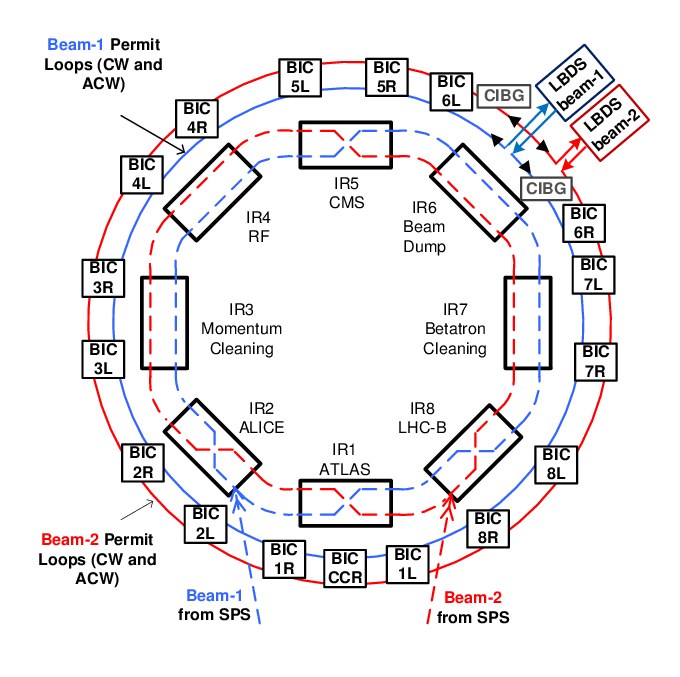
\includegraphics[width=0.75\textwidth]{LHC-beam-permit-loops}\\
  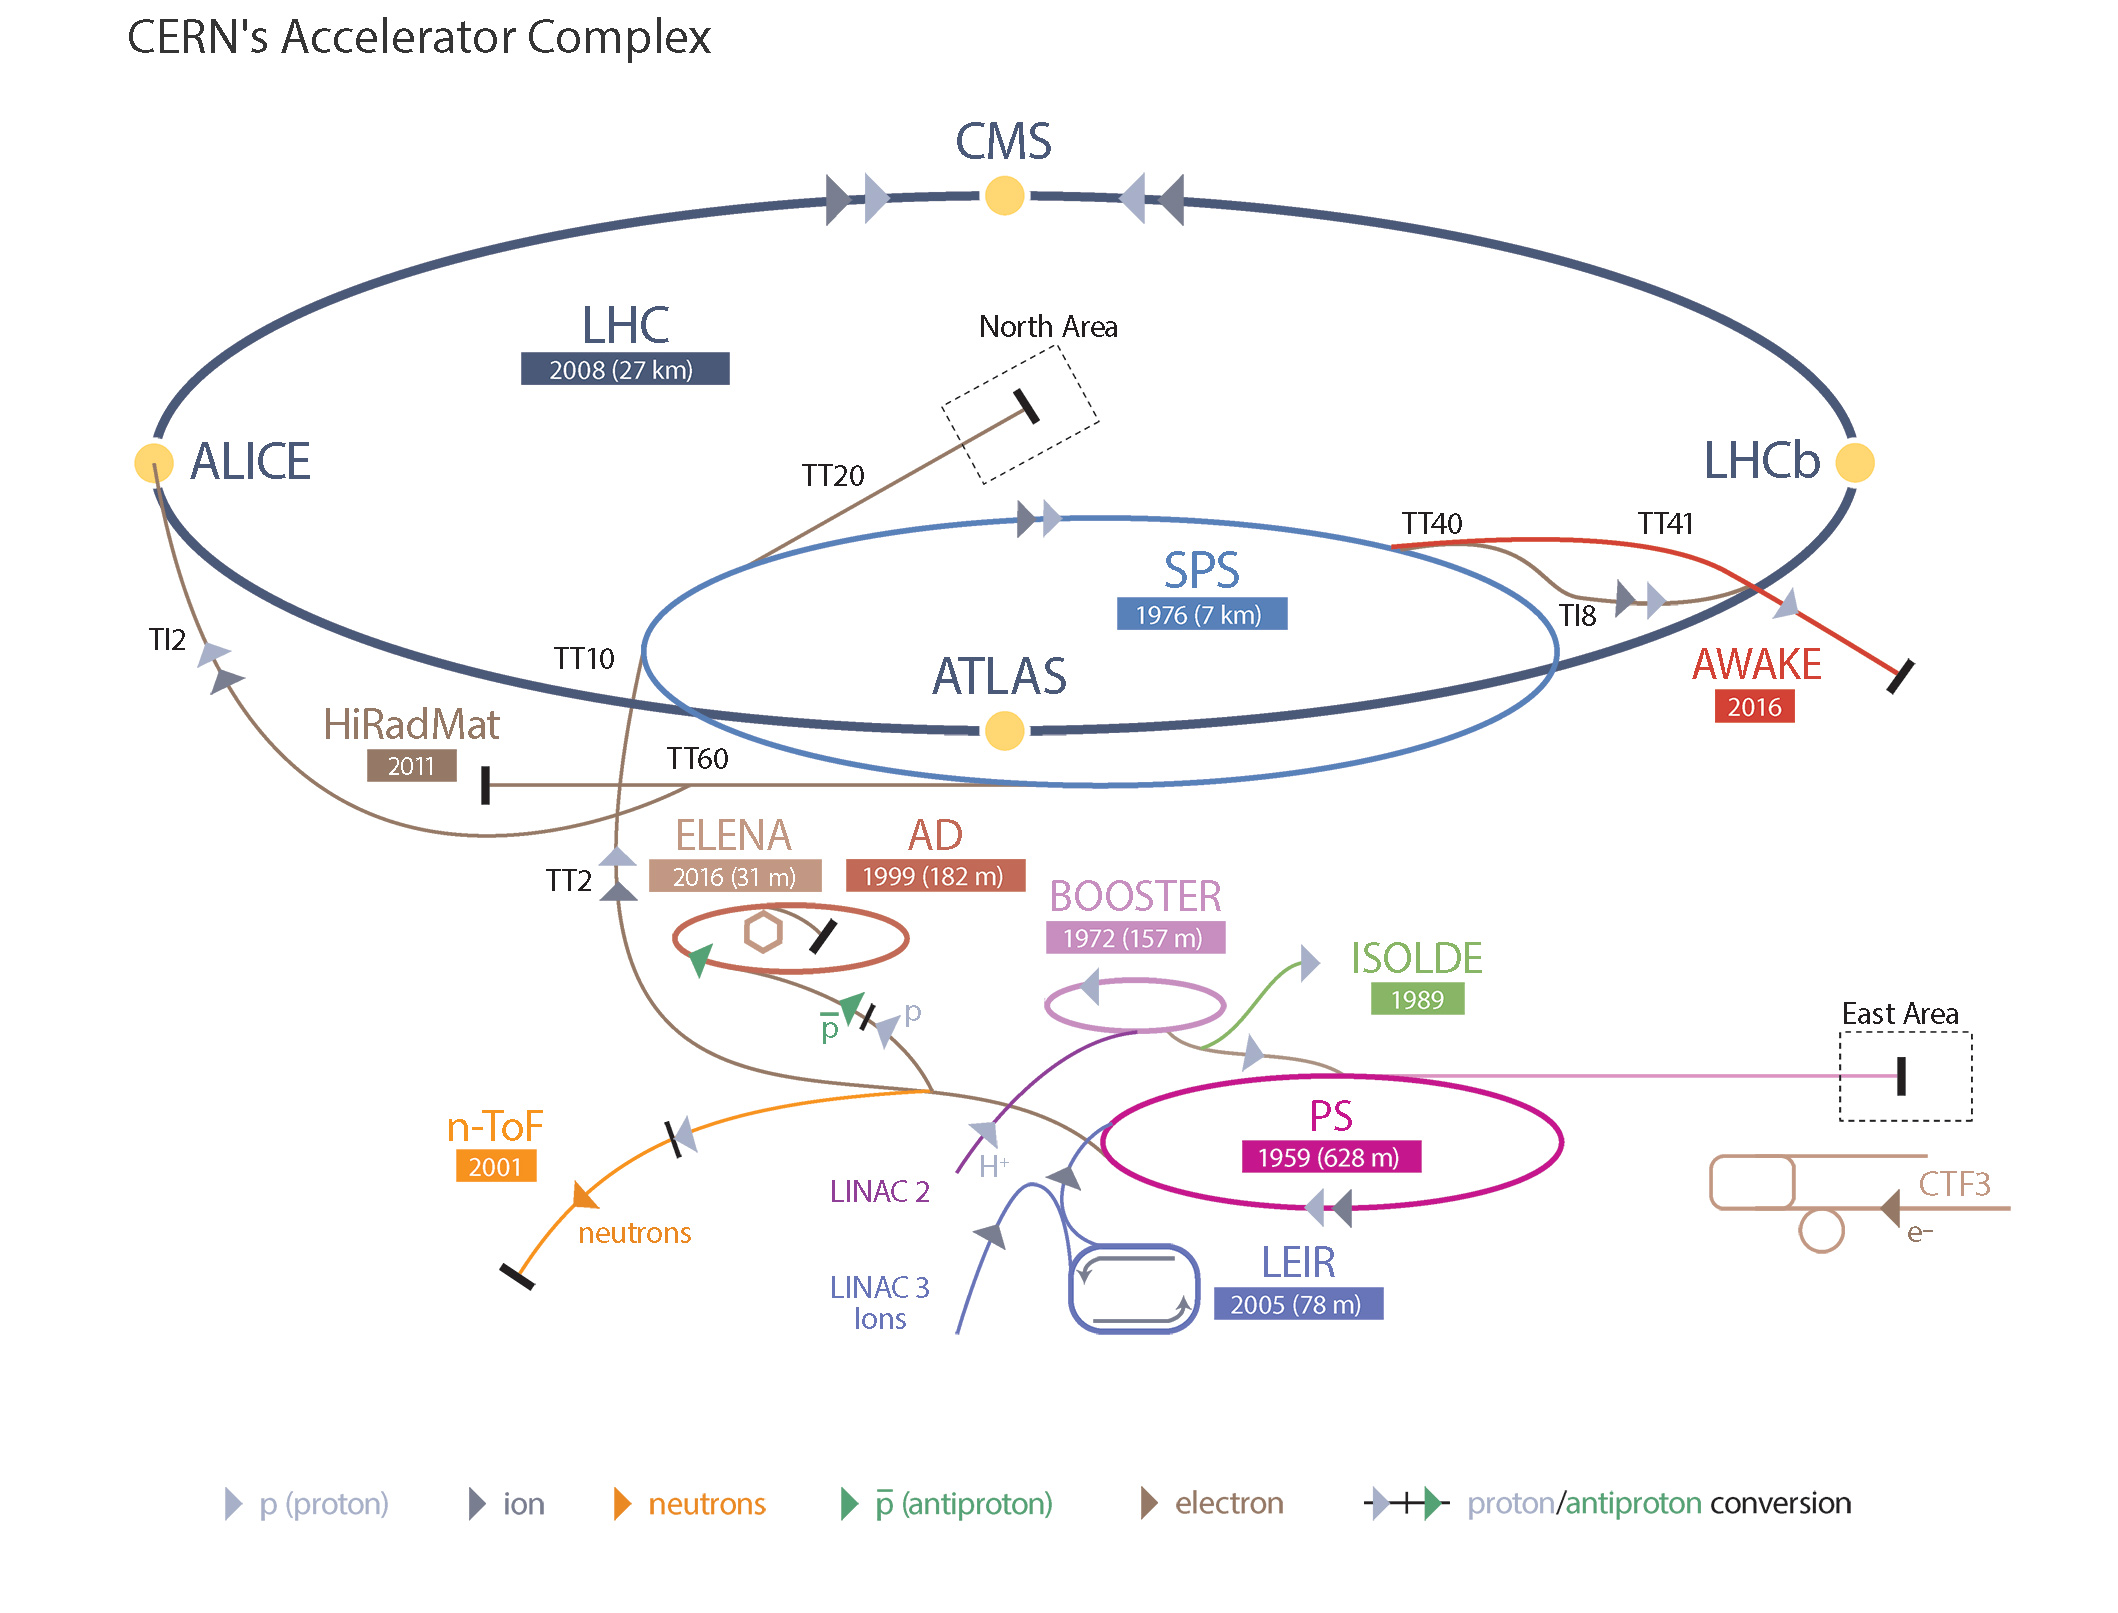
\includegraphics[width=0.75\textwidth]{LHC_default.jpg}
  \caption {Schematic layout of the LHC.}
  \label{lhcmap}
\end{figure}


\section{The LHC}\label{sec:lhc}
The first LHC budget plan was approved in 1996 and the final cost sum was completed in 2008. 4 years later the Higgs discovery happened, in 2012, quite fast for such a huge project! 
Now we will talk about the most important parts of the LHC complex one-by-one. Let us start with magnets. 

 
\subsection{The Magnets}\label{sec:magnets}
To keep the beam of protons on a circular orbit LHC needs strong magnets. The proven technology existed since Tevatron and relied on $NbTi$ superconductors. 1232 dipoles at 8 $T$, which are cooled to the below 2 $K$ temperature using superfluid Helium, bend the beam \ref{lhcDipole}. The dipole cold mass is in the so-called Helium bath and is cooled down to 1.9 $K$. Each of the 16.5 $m$ (with ancillaries) long and 570 $mm$ in diameter dipoles is slightly curved by 5.1 $mrad$ to help a chain of dipoles complete 360 degrees. The dipole is located inside of the dipole cryostat, which is a long cylindrical tube 914 $mm$ in diameter made of low-carbon steel. During the standard operation time the vessel contains the vacuum. 



\begin{figure}[H]
  \centering
  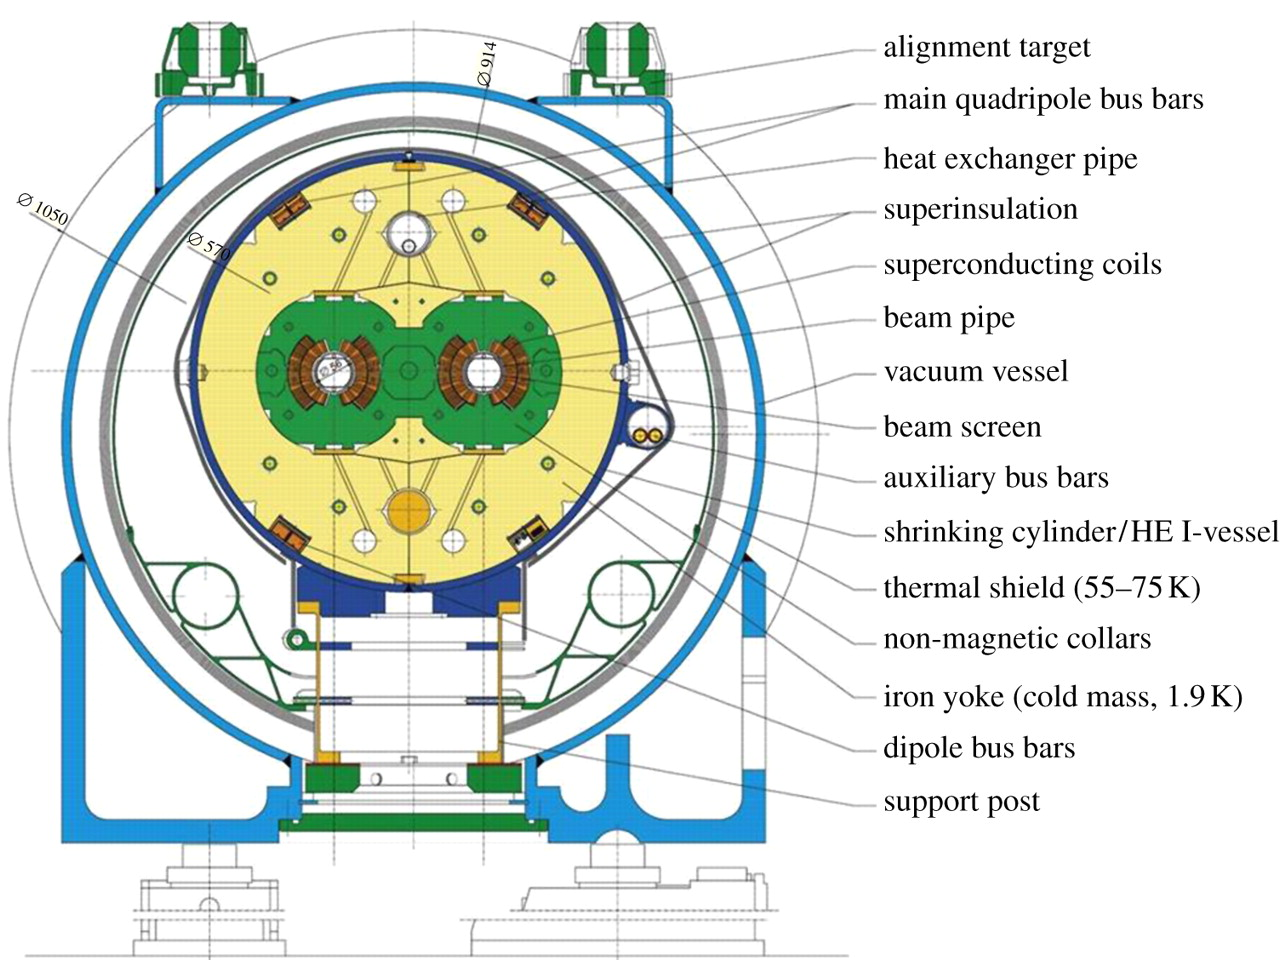
\includegraphics[width=0.9\textwidth]{lhcDipole}
  \caption[The cross section of the LHC dipole]{The cross section of the LHC dipole.}\label{lhcDipole}
\end{figure}


The material and the properties of the cables for the dipoles had to be carefully chosen. Each dipole coil is 56 $mm$ in diameter and is made of cables of two types. The cable in the inner layer contains 28 strands 1.065 $mm$ each. The outer layer contains 36 strands 0.825 $mm$ each \ref{cables}. 

To correct the orbit, higher order correctors are used with about 3800 single aperture and 1000 twin aperture magnets evenly spaces around the circular trajectory. 

Another important task that is performed with the use of magnets is the beam insertion, which is done at eight specific insertion locations. LHC also uses $NbTi$ magnets to accomplish this work. 


\begin{figure}[H]
  \centering
  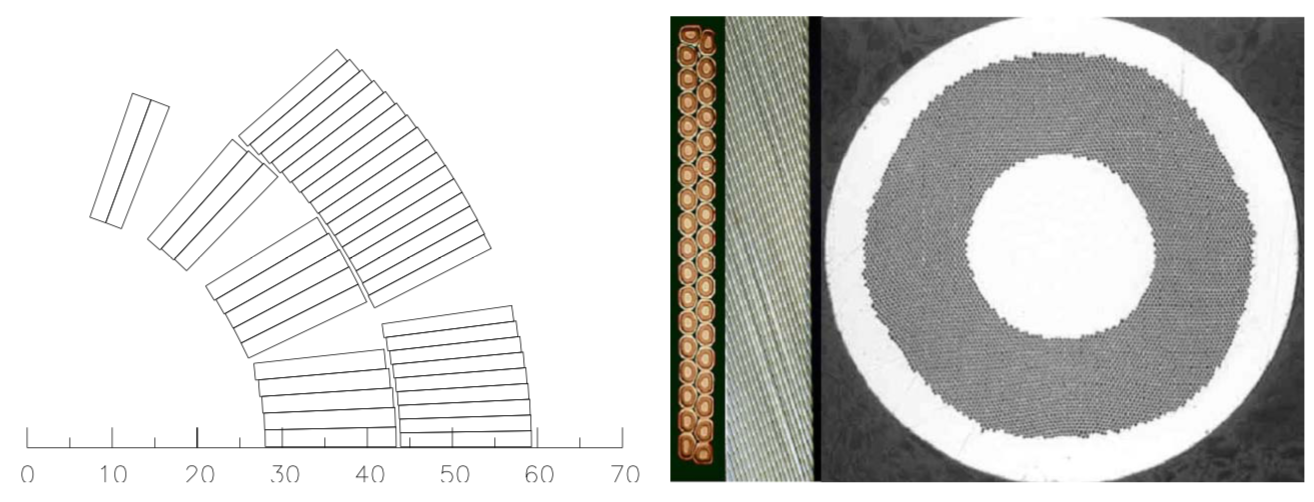
\includegraphics[width=0.9\textwidth]{cables}
  \caption[Cables of the dipole magnet]{Cables of the dipole magnet. Left: cross section view. Right: Strand and cables}\label{cables}
\end{figure}



\subsection{Radio Frequency System}\label{sec:rf}

The beam that comes from injectors will be placed, accelerated and kept on the orbit with the help of Radio Frequency (RF) cavities. The same system will be used to correct for injection errors in the beam direction. RF will be operating at the 400 $MHz$, which is 10 times more than the revolution frequency of 40 $MHz$. 

Four RF cavities grouped together into one cryomodule constitute an important accelerating module. If something happens to this module, it can be easily replaced in short period of time. 


\begin{figure}[H]
\centering
%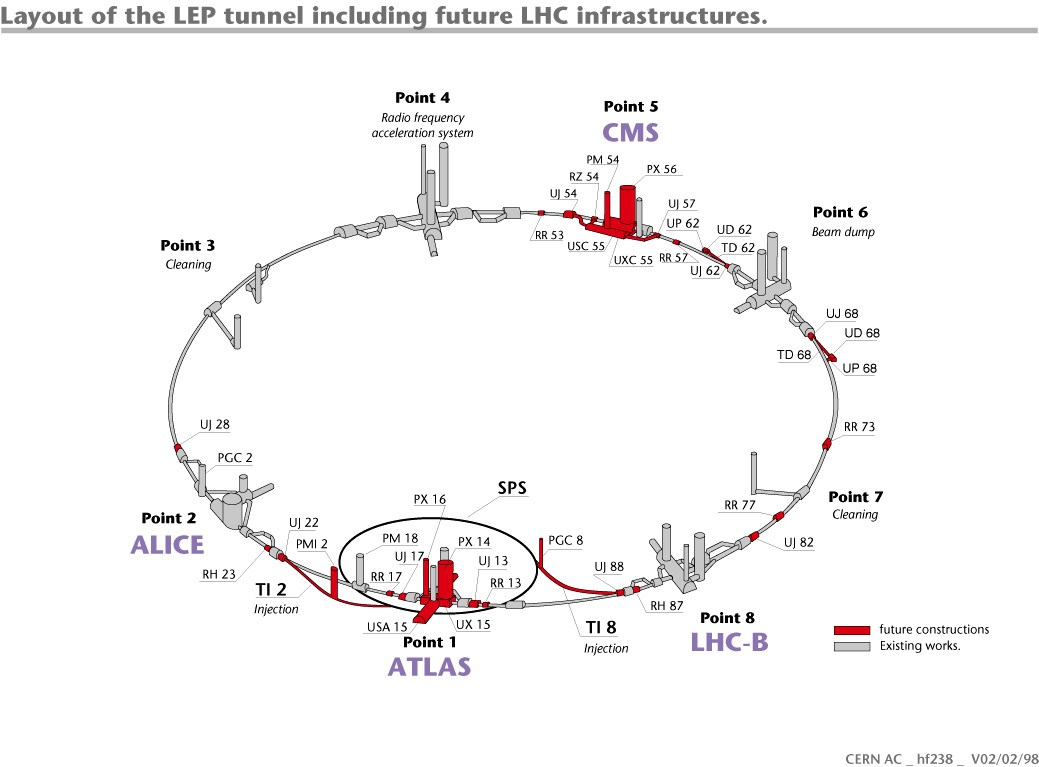
\includegraphics[scale=0.6]{lep}
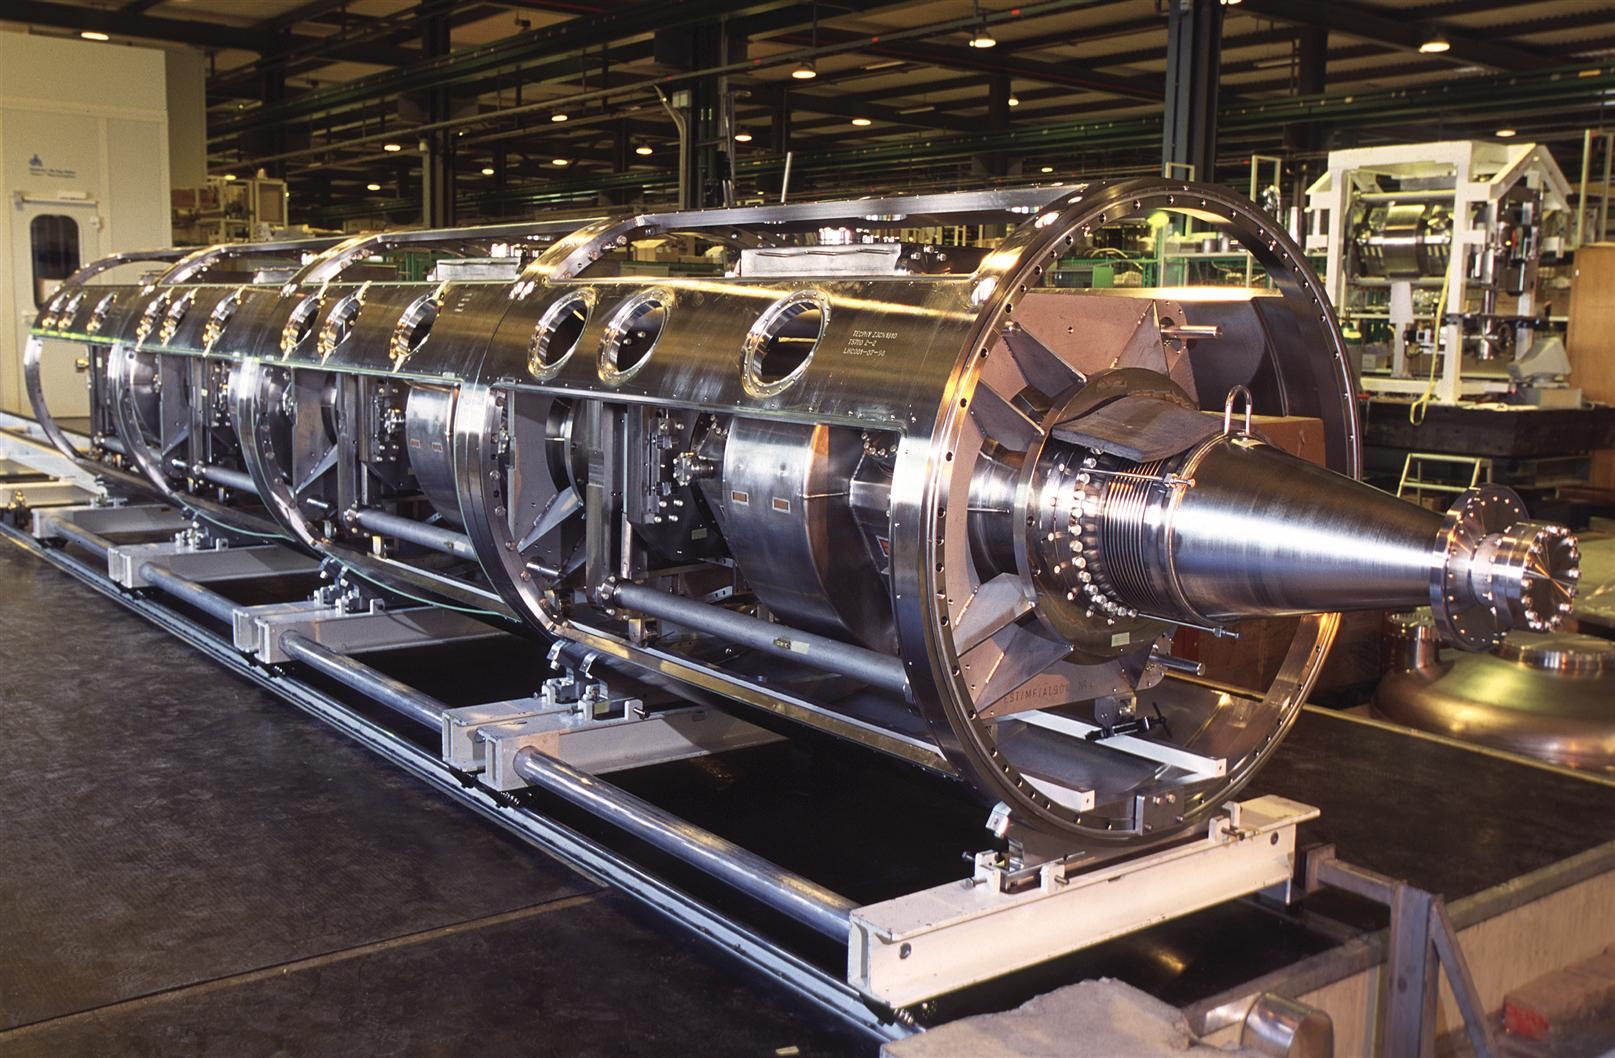
\includegraphics[width=7cm,height=4.2cm]{lhc_rfc}
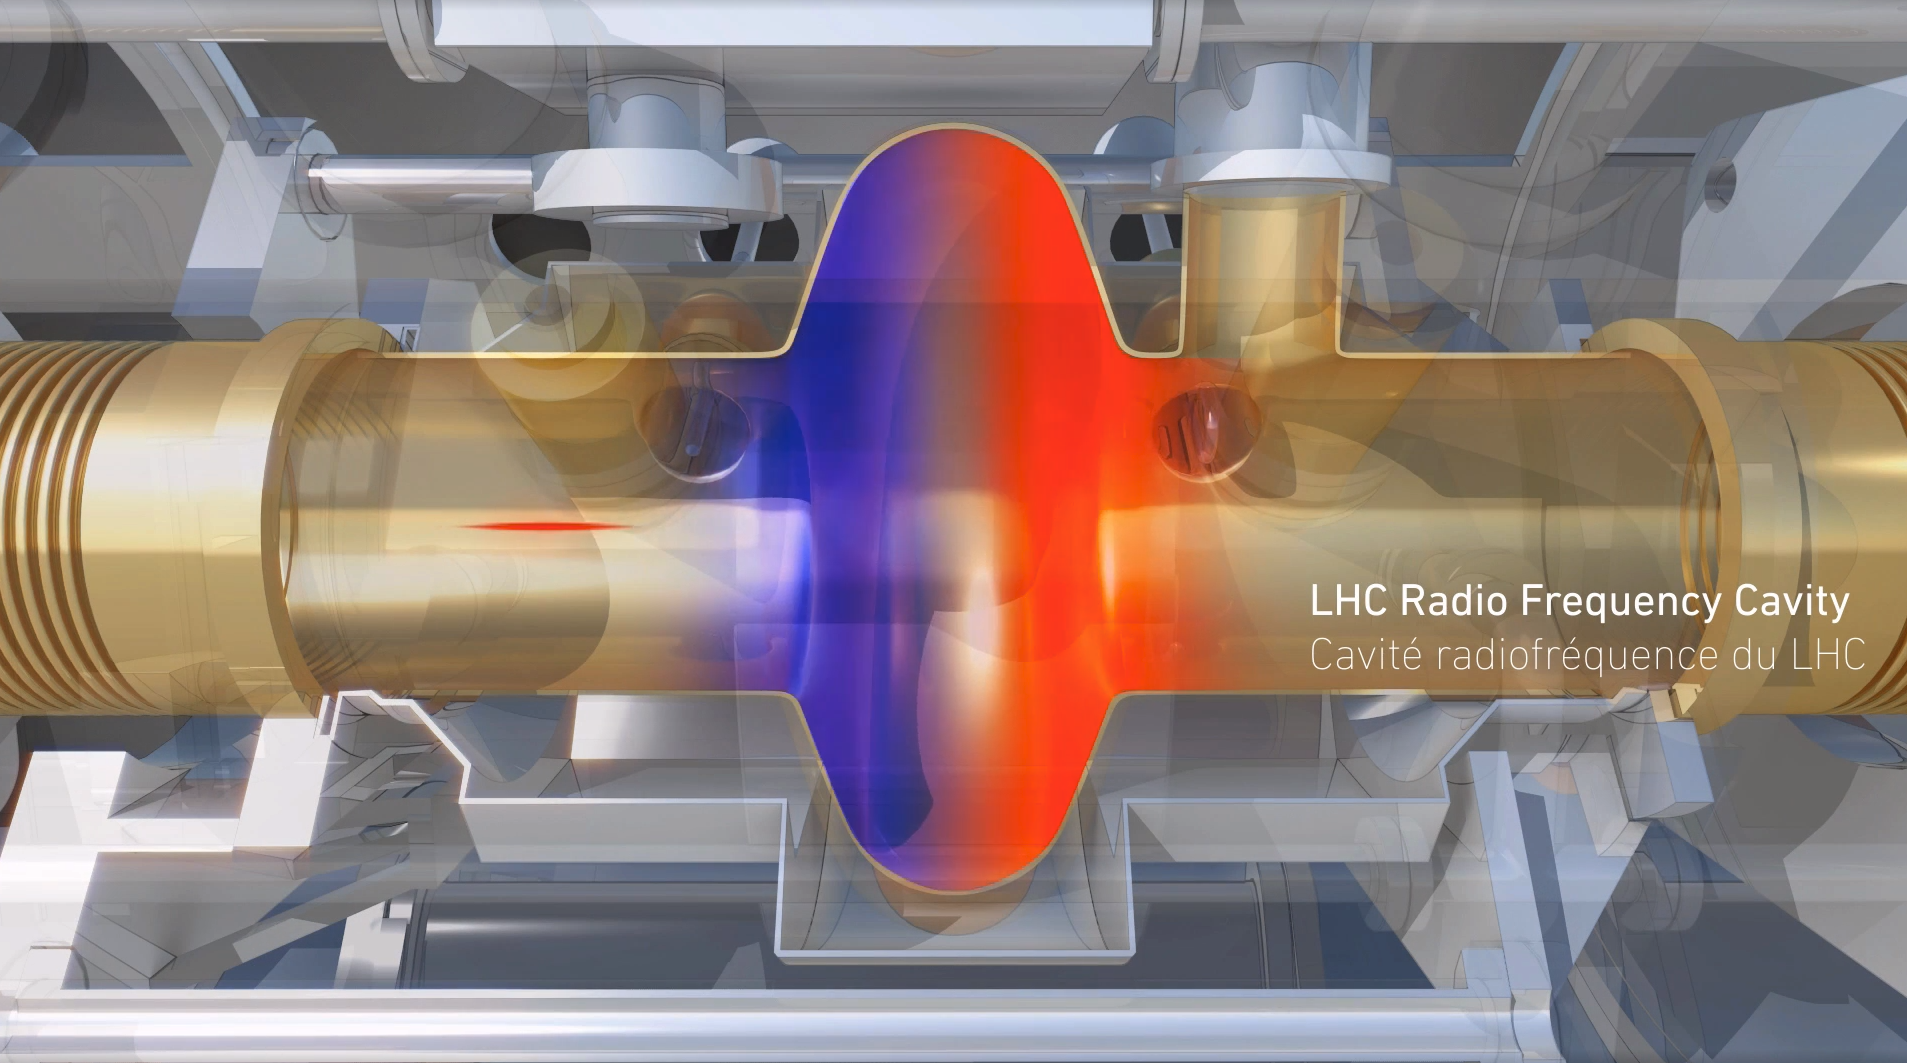
\includegraphics[scale=0.15]{rfc_lhc}
\caption[RF cavities module.]{LHC RF cavities. Right: a single RF cavity schematic drawing. The colour field is used to highlight the fact of two field of the different polarity. Left: a cryomodule with four RF cavities.}
\end{figure}


\subsection{Vacuum System}\label{sec:vacuum}


Three types of vacuum systems are necessary for the LHC proper operation. The vacuum system for the cryomagnets, the insulation vacuum for helium distribution, and, of course, the vacuum for the beam (VBS). As a convention, taking into account ionisation cross sections for gasses of the interests, cryogenic temperatures are expressed as corresponding gas densities normalised to the hydrogen. 
VBS, to ensure the 100 hours long run time, requires the equivalent hydrogen densities (EHD) to be below $10^{15} H_2 \frac{1}{m^3}$. To minimise the backgrounds from the experiments, the EHD at the interaction points should be $10^{13} H_2 \frac{1}{m^3}$. Those parts of the beam system, which operate under room temperatures, are under the pressure of $10^{-10}$ to $ 10^{-11}$ $ m$bar. All the vacuum section are subdivided into smaller modules to allow easy repair and fine tuning. 
VBS, as the most demanding in terms of the vacuum quality, have to be properly designed and must address a number of challenges, such as synchrotron radiation that significantly affects vacuum chambers in the arcs around the tunnel, as well as an electron cloud effect which exists along the length of the whole circle of the LHC. After the beam is inserted and is stabilised, the final adjustment of the VBS is needed to guarantee the perfect performance.

To finish the discussion of the VBS, let us discuss which heat sources have the main effect on the vacuum of the beam that must exist at the 1.9 K. 

\begin{itemize}
\item Synchrotron radiation (0.2 $W/m$ per beam)
\item Energy loss by nuclear scattering (30 $mW/m$ per beam)
\item Image currents (0.2 $W/m$ per beam)
\item Electron cloud related effects (vary)
\end{itemize}

To obstruct the heat sources mentioned above, specific beam screens are developed. Screens have elliptical shape, so-called racetrack shape, which gives extra space for cooling while optimises the aperture. 
Finally, the lifetime of the vacuum is mostly determined by the interactions of the vacuum gas nuclei with the protons of the beam. Values of the cross sections of such processes are given in \ref{Eggert:260711, Gr�bner:356437}.


\begin{figure}[H]
  \centering
  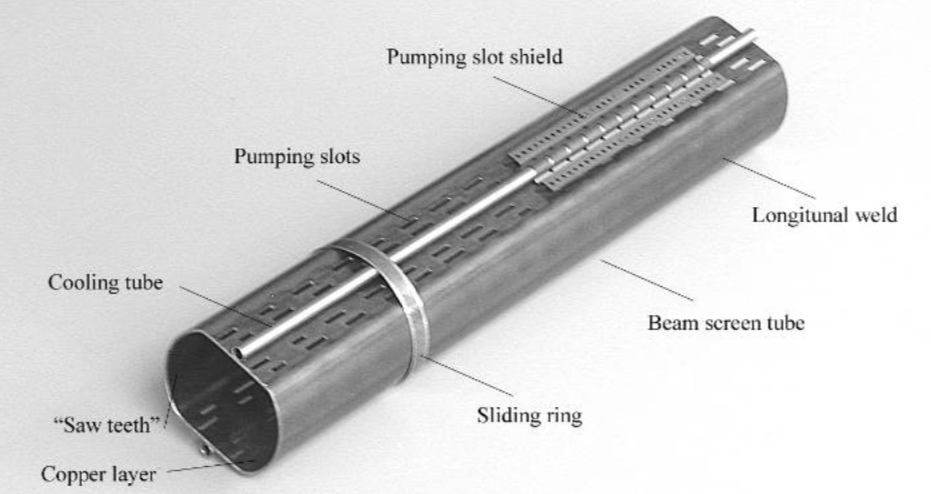
\includegraphics[width=0.7\textwidth]{beam_screen}
  \caption{Beam screen.}\label{fig:beam_screen}
\end{figure}

\subsection{Powering}\label{sec:power}
To power the LHC, 1612 electrical circuits of 131 types are used. The magnets are powered in eight symmetrical sections. Some sections rely on all 131 types of circuits, while others may use only specific ones. To power the main quadrupoles which focus the beam, the power converters are located in the underground area. 
A total of 3286 current leads is needed to connect all the circuits and power cables. 1070 of the leads operate between 600 A and 13 kA. The other leads work in the range 60 to 120 A. 

\begin{figure}[H]
  \centering
  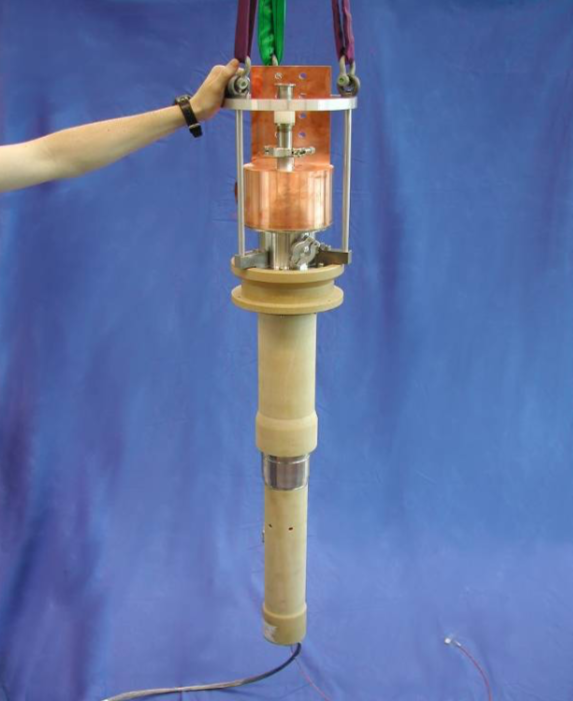
\includegraphics[width=0.7\textwidth]{13kA_lead}
  \caption{13 kA high-temperature superconducting current lead.}\label{fig:13kA_lead}
\end{figure}


\subsection{Cryogenic system}\label{sec:cryogenic}
The cryogenic system must supply the LHC cold mass of 37 Mkg within 15 days with the necessary temperature settings and work with the temperatures different by 75 K. The system must also be able to deal with the fast pressure raises and flow surges, and should be able to recover in a short period of time from such perturbations not to affect the run of the whole LHC. Another important point during the cryogenic design that had to be addressed is the fact that the LHC tunnel is inclined in the horizontal plane by 1.41 $^\circ$. This equals to 120 m difference in the vertical location of two diametrically opposite points of the tunnel with respect to the surface level and results in the additional hydrostatic pressure that can affect the flow of the cryogen. To avoid any instability of the LHC work like this, the gas is transported in the super-heated-vapour state. 

\begin{figure}[H]
  \centering
  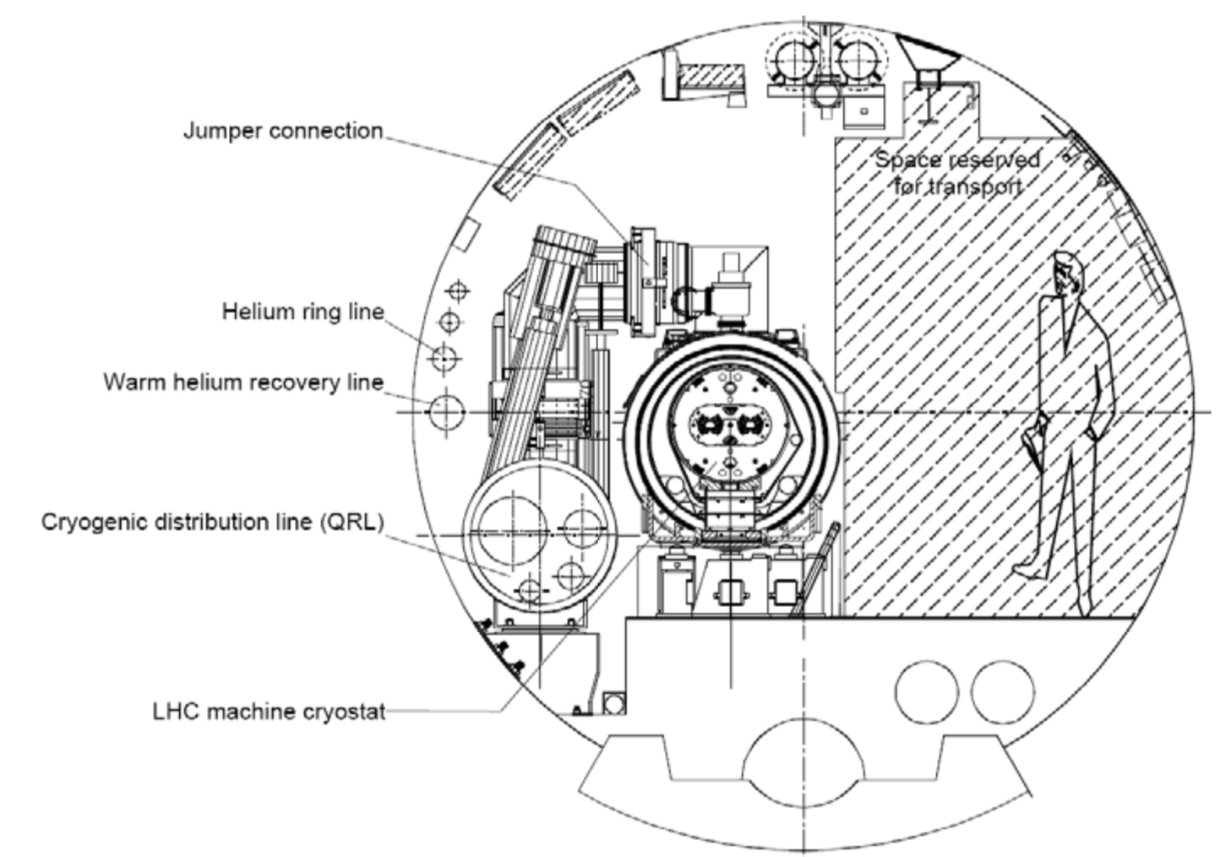
\includegraphics[width=0.7\textwidth]{cryo}
  \caption{Cross section of the LHC tunnel}\label{fig:cryo}
\end{figure}


Since the cost of the production of 1.8 K temperature is high, several temperature levels are employed:
 
\begin{itemize}
\item 50 to 75 K to the thermal shielding that protects the cold masses
\item 4.6 to 20 K for lower temperature interception and to cool the beam screens
\item 1.9 K for quasi-isotermal helium in the superfluid state to cool the magnet cold mass
\item 4 K for the transportation system that directs the 1.8 K helium from the exchanger to the 1.8 K refrigerator 
\item 4.5 K for RF cavities and lower sections of the high-temperature superconducting current leads
\item 20 to 300 K for upper sections of the high-temperature superconducting current leads
\end{itemize}

\begin{figure}[H]
  \centering
  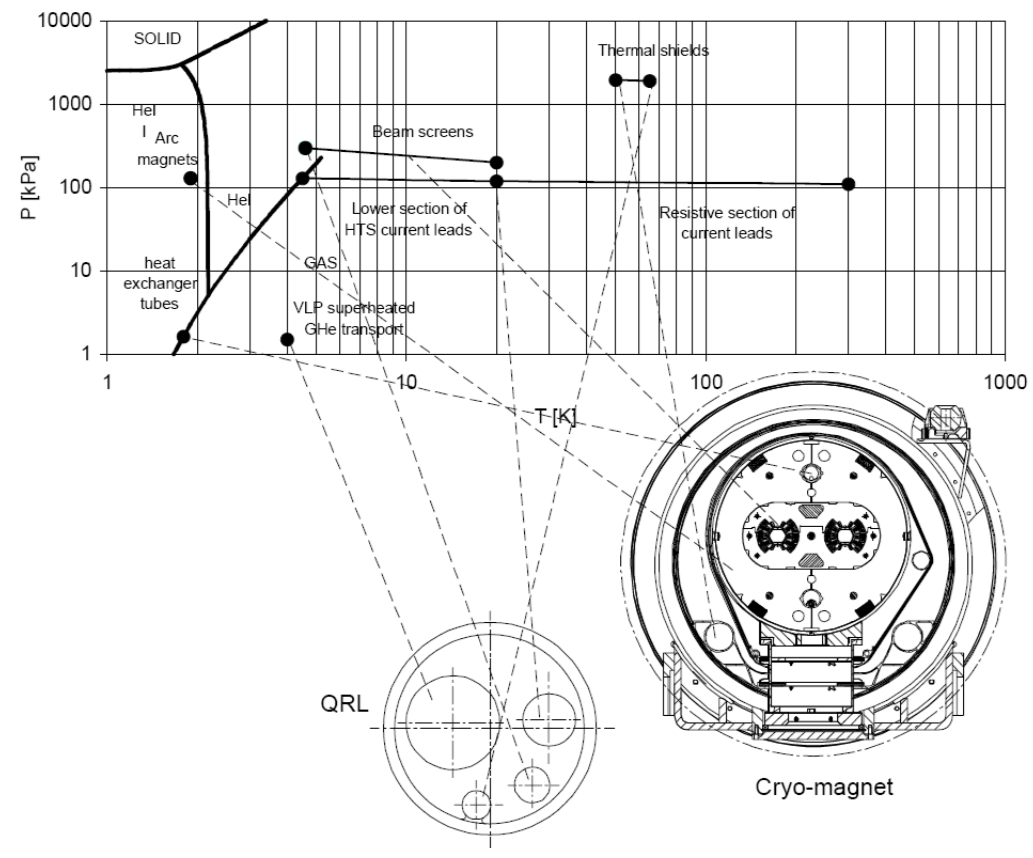
\includegraphics[width=0.7\textwidth]{cryo_T_scale}
  \caption{LHC cryogenic states and the temperature scale.}\label{fig:cryo_T_scale}
\end{figure}

\newpage






















 	 


\begin{figure}[H]
  \centering
  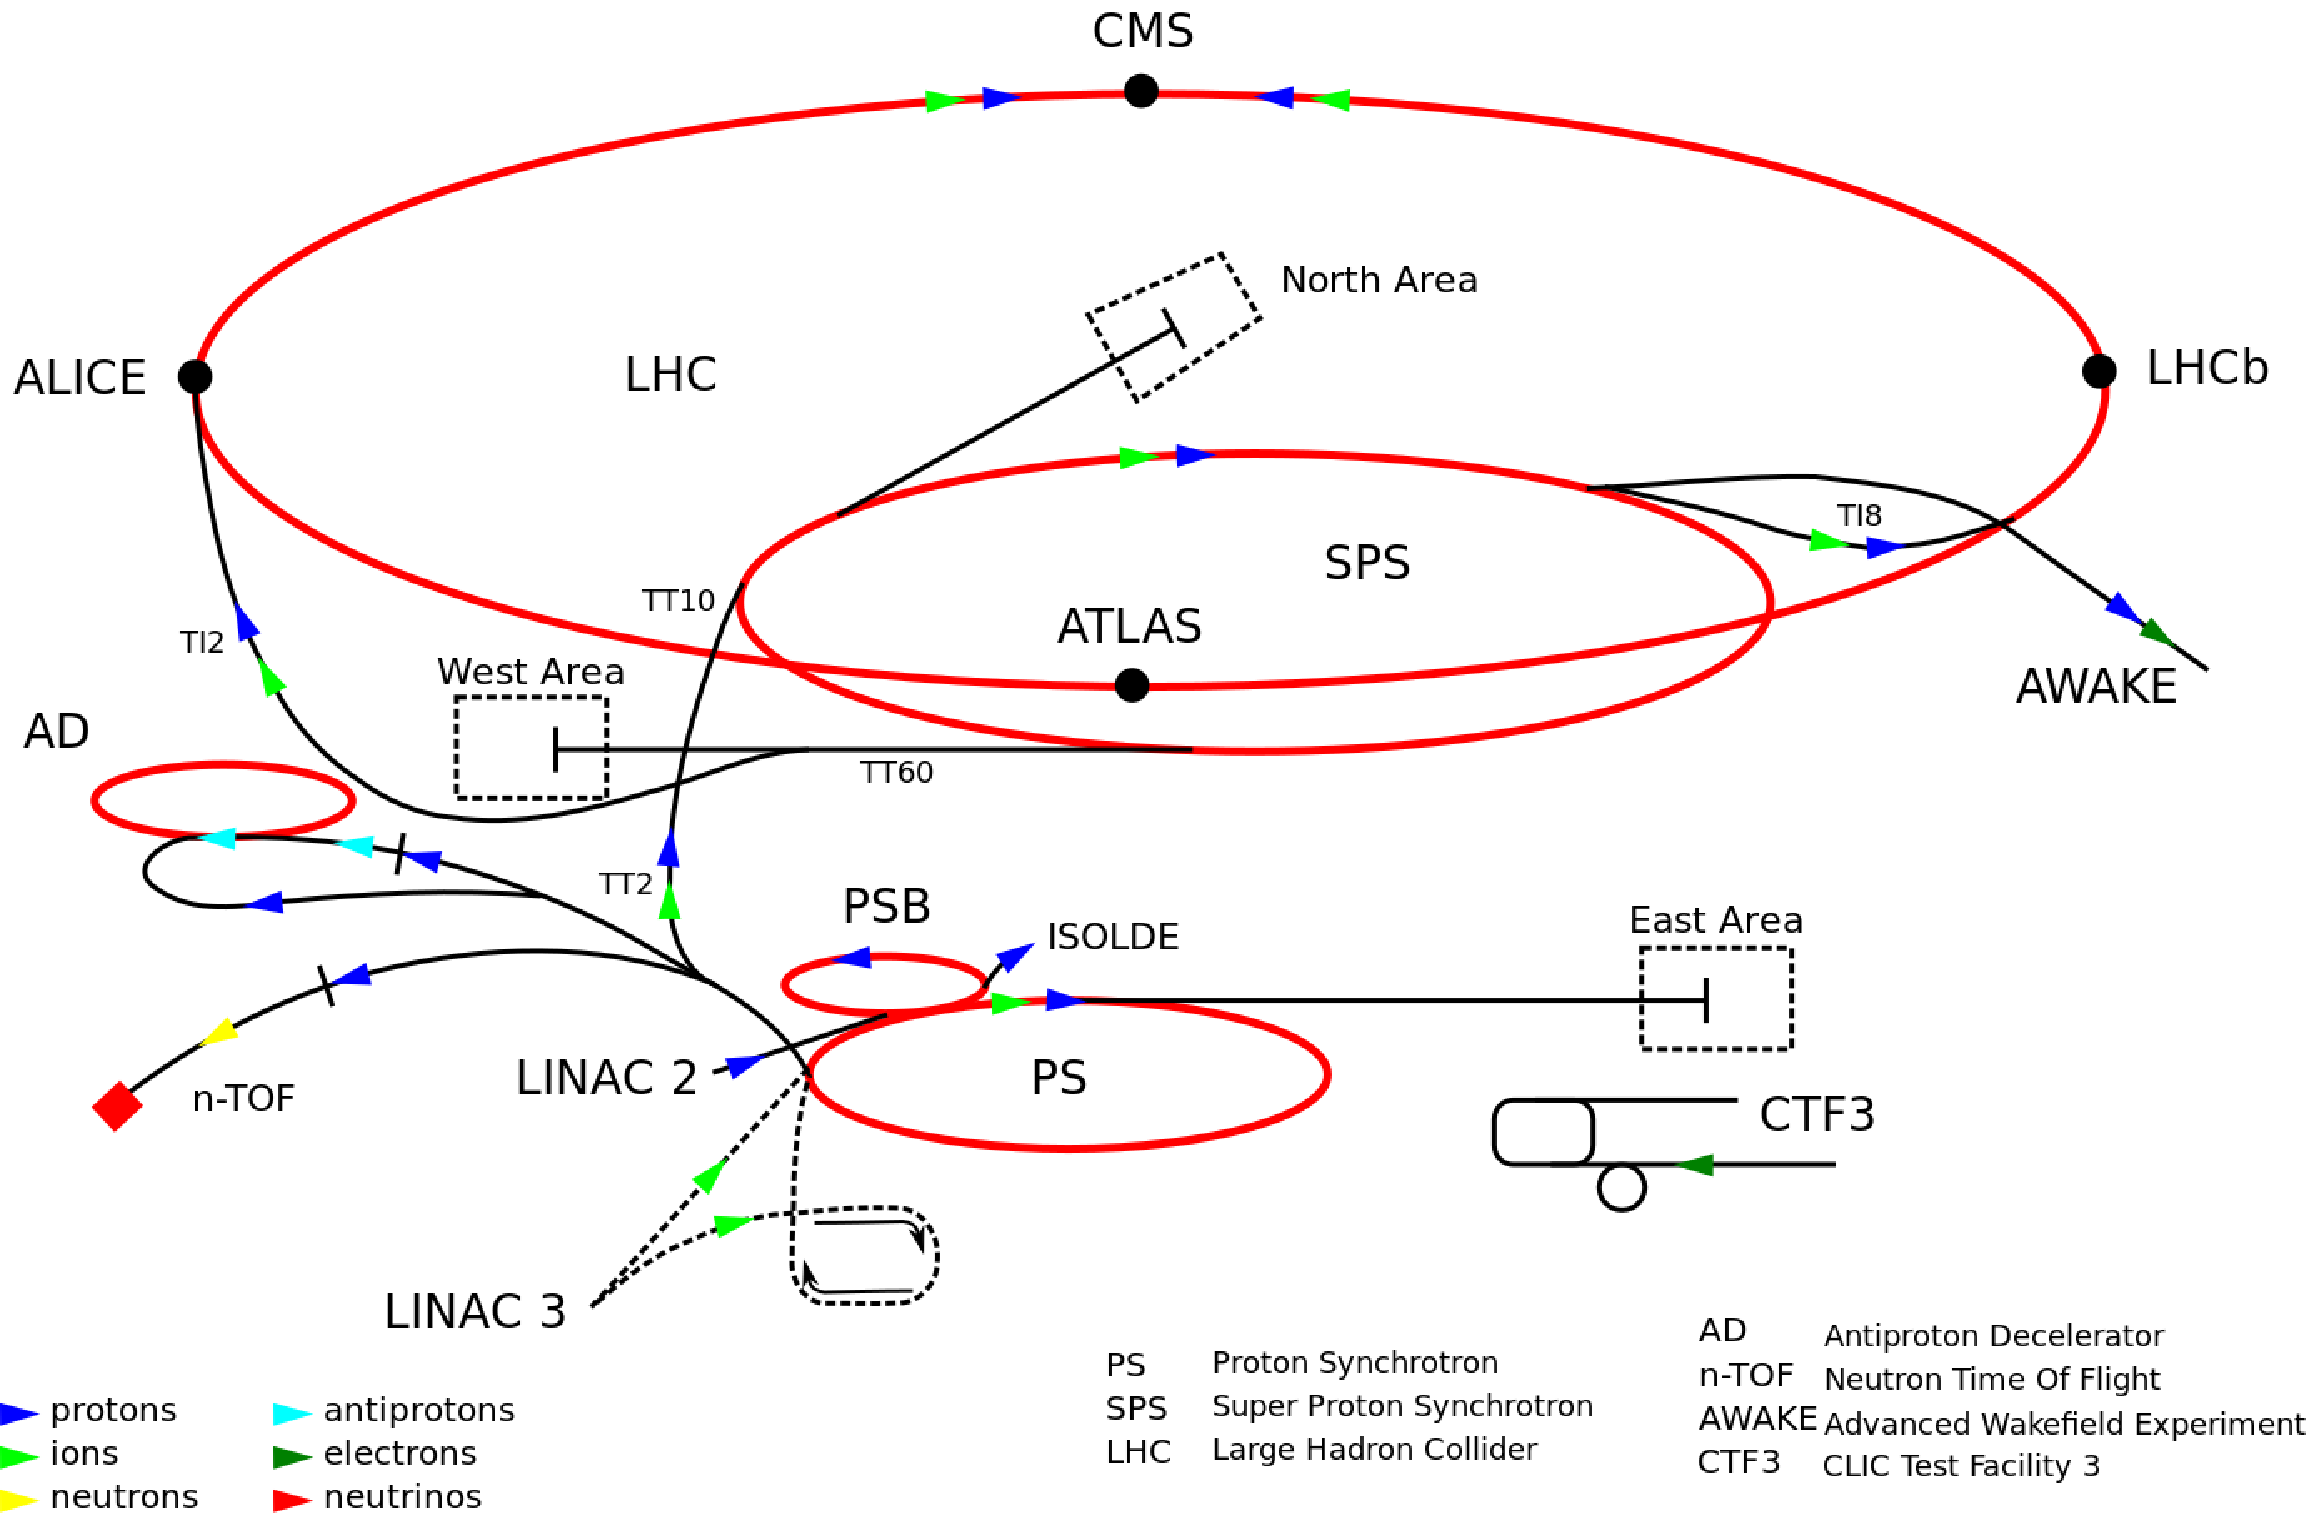
\includegraphics[width=0.7\textwidth]{cern_ac}
  \caption[CERN accelerator complex]{CERN accelerator complex. Blue arrows show the path followed by protons along the acceleration process \cite{cern}.}\label{fig:cern}
\end{figure}

The LHC runs in three collision modes depending on the particles being accelerated

\begin{itemize}
\item Proton-Proton collisions (\pp) for multiple physics experiments.
\item Lead-Lead collisions (Pb-Pb) for heavy ion experiments. 
\item Proton-Lead collisions (p-Pb) for quark-gluon plasma experiments.
\end{itemize}

\begin{figure}[!h]
\centering
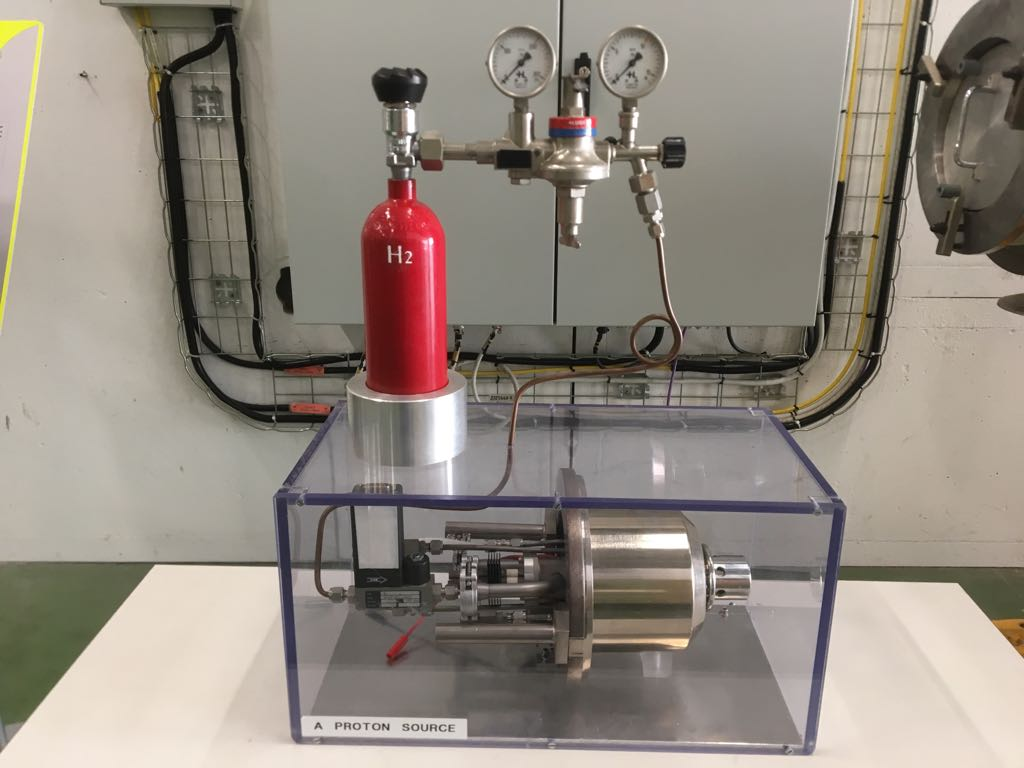
\includegraphics[width=4.5cm,height=3.3cm]{hbottle}
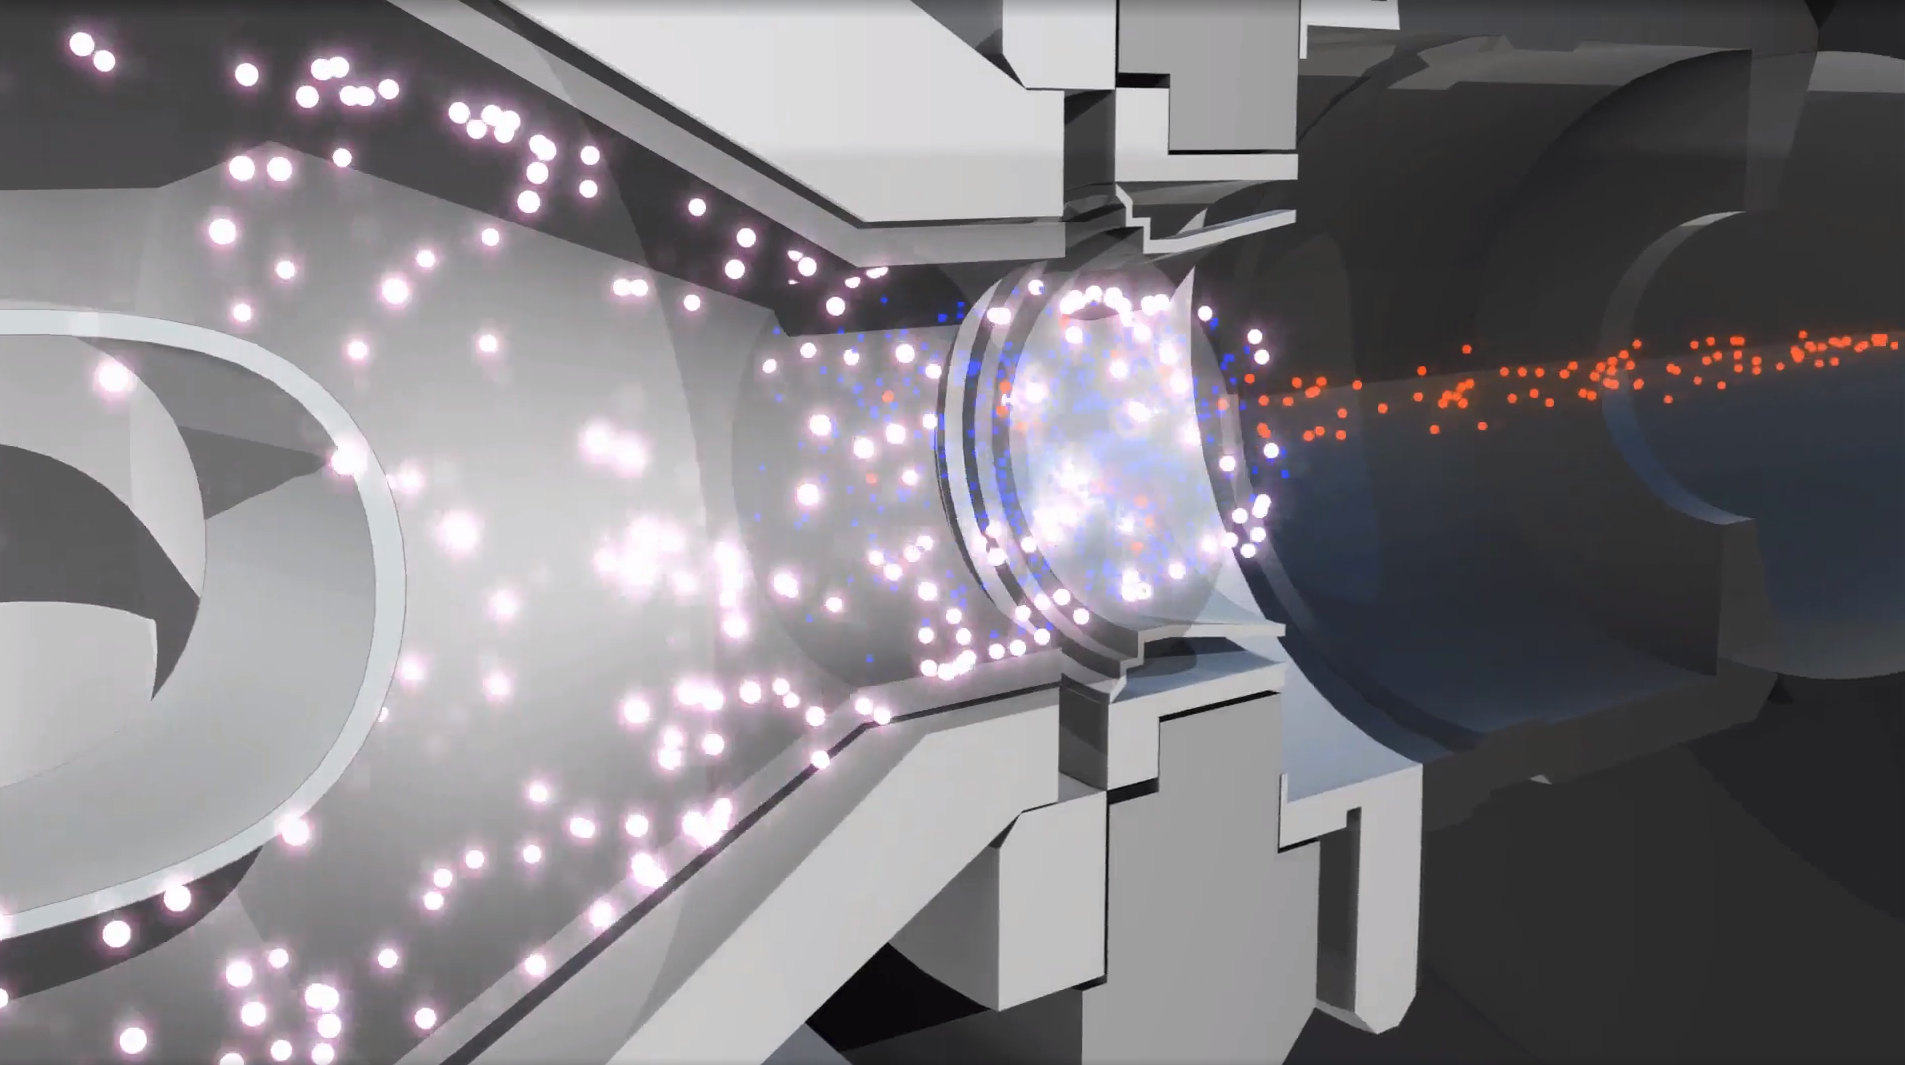
\includegraphics[width=6.0cm,height=3.3cm]{proton_source}\\
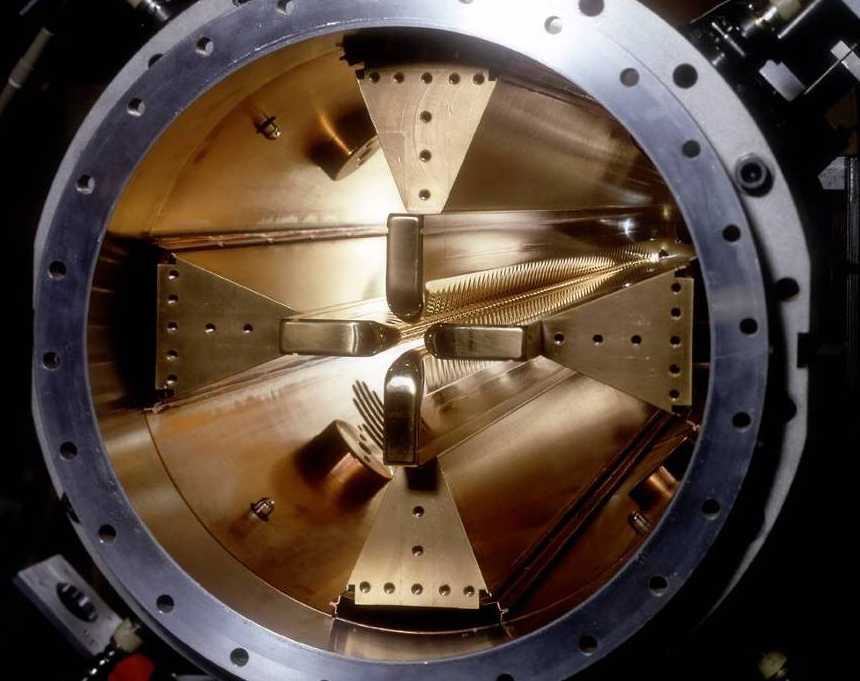
\includegraphics[width=4.5cm,height=3.3cm]{rfq2}
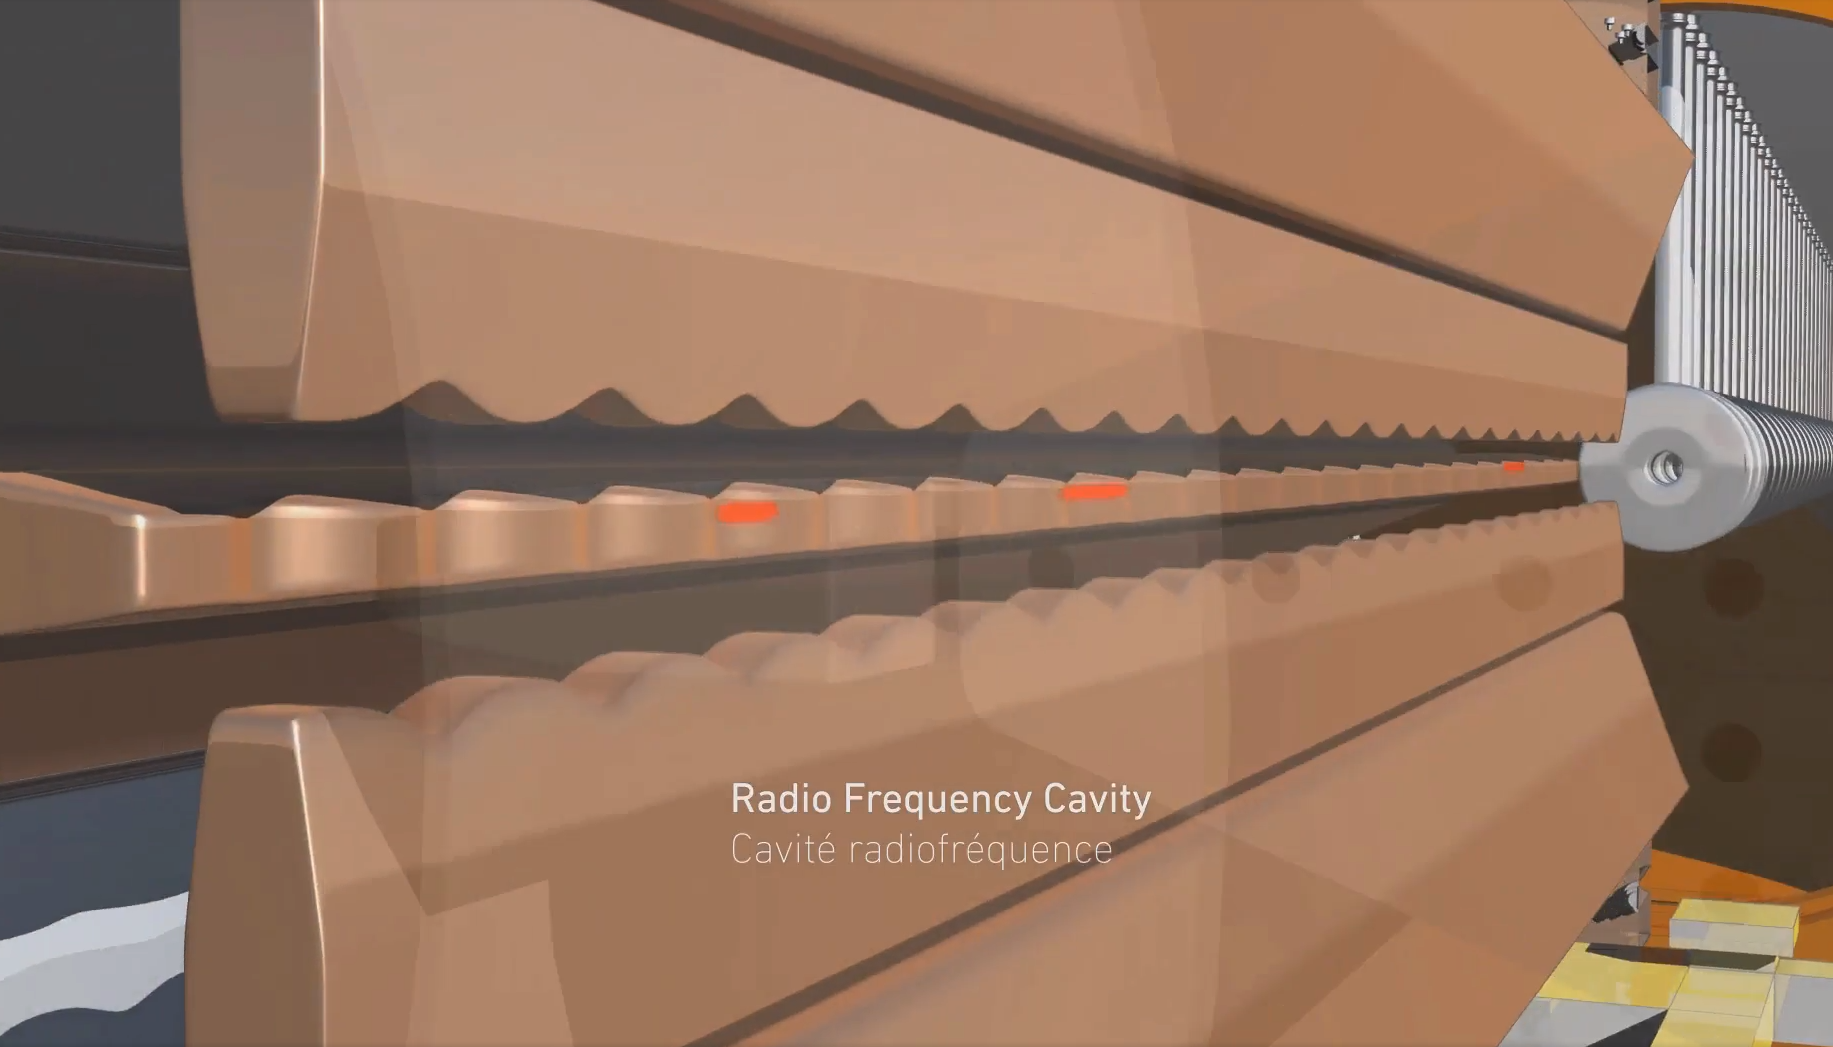
\includegraphics[width=6.0cm,height=3.3cm]{rfq3}
\caption[LHC protons source. First acceleration stage.]{LHC protons source and the first acceleration stage. Top: the bottle contains hydrogen gas which is injected into the metal cylinder (white dots) to be broken down into electrons (blue dots) and protons (red dots); Bottom: the obtained protons are directed towards the radio frequency quadrupole which perform the first acceleration, focus the beam and create the bunches of protons. Letf images are real pictures while right images are drawings \cite{rfq2,video}.}\label{fig:hbottle}
\end{figure}

\noindent In this thesis only \pp collisions will be considered.

Collection of protons starts with hydrogen atoms taken from a bottle, containing hydrogen gas, and injecting them in a metal cylinder; hydrogen atoms are broken down into electrons and protons by an intense electric field (see Figure \ref{fig:hbottle} top). The resulting protons leave the metal cylinder towards a radio frequency quadrupole (RFQ) that focus the beam, accelerates the protons and creates the packets of protons called bunches. In the RFQ, an electric field is generated by a RF wave at a frequency that matches the resonance frequency of the cavity where the electrodes are contained. The beam of protons traveling on the RFQ axis experiences an alternating electric field gradient that generates the focusing forces.

In order to accelerate the protons, a longitudinal time-varying electric field component is added to the system; it is done by giving the electrodes a sine-like profile as shown in Figure \ref{fig:hbottle} bottom. By matching the speed and phase of the protons with the longitudinal electric field the bunching is performed; protons synchronized with the RFQ (synchronous protons) do not feel an accelerating force, but those protons in the beam that have more (or less) energy than the synchronous proton (asynchronous protons) will feel a decelerating (accelerating) force; therefore, asynchronous protons will oscillate around the synchronous ones forming bunches of protons \cite{rfq}. From the RFQ protons emerge with energy 750 keV in bunches of about $1.15 \times 10^{11}$ protons \cite{lyndon}.        

\begin{figure}[!h]
  \centering
  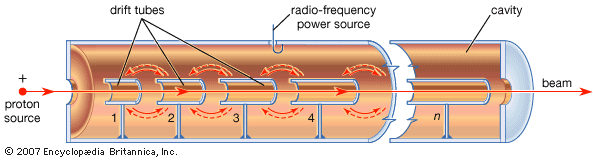
\includegraphics[width=0.65\textwidth,height=3.5cm]{linac}
  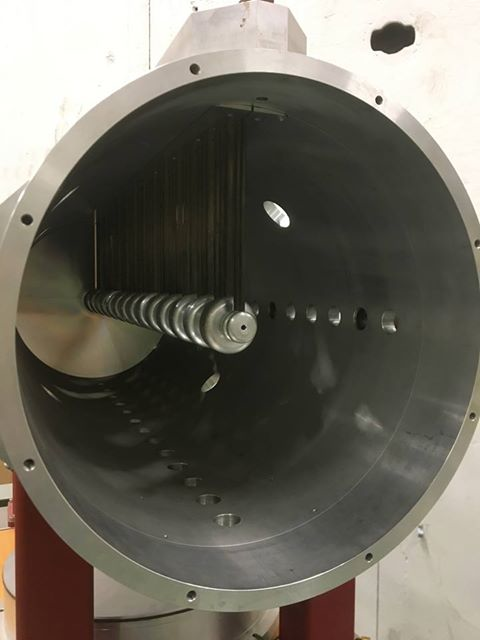
\includegraphics[width=0.3\textwidth,height=3.5cm]{linac2}
  \caption [The LINAC2 accelerating system at CERN.]{ Left: drawing of the LINAC2 accelerating system at CERN. Electric fields generated by radio frequency (RF) create acceleration and deceleration zones inside the cavity; deceleration zones are blocked by drift tubes where quadrupole magnets focus the proton beam. Right: picture of a real RF cavity \cite{linac}.}\label{fig:linac}
\end{figure}

Proton bunches coming from the RFQ go to the linear accelerator 2 (LINAC2) where they are accelerated to reach 50 MeV energy. In the LINAC2 stage, acceleration is performed using electric fields generated by radio frequency which create zones of acceleration and deceleration as shown in Figure \ref{fig:linac}. In the deceleration zones, the electric field is blocked using drift tubes where protons are free to drift while quadrupole magnets focus the beam.   

The beam coming from LINAC2 is injected into the proton synchrotron booster (PSB) to reach 1.4 GeV in energy. The next acceleration is provided at the proton synchrotron (PS) up to 26 GeV, followed by the injection into the super proton synchrotron (SPS) where protons are accelerated to 450 GeV. Finally, protons are injected into the LHC where they are accelerated to the target energy of 6.5 TeV.

PSB, PS, SPS and LHC accelerate protons using the same RF acceleration technique described before. 










The LHC has a system of 16 RF cavities located in the so-called point 4, as shown in Figure \ref{fig:lep_rfc} top, tuned at a frequency of 400 MHz. The bottom side of Figure \ref{fig:lep_rfc} shows a picture of a RF module composed of 4 RF cavities working in a superconducting state at 4.5 K; also, a representation of the accelerating electric field that accelerates the protons in the bunch is shown. The maximum of the oscillating electric field (red region) picks the proton bunches at the the entrance of the cavity and keeps accelerating them through the whole cavity. The protons are carefully timed so that in addition to the acceleration effect the bunch structure of the beam is preserved.    

While protons are accelerated in one section of the LHC ring, where the RF cavities are located, in the rest of their path they have to be kept in the curved trajectory defined by the LHC ring. Technically, LHC is not a perfect circle; RF, injection, beam dumping, beam cleaning and sections before and after the experimental points where protons collide are all straight sections. In total, there are 8 arcs 2.45 km long each and 8 straight sections 545 m long each. In order to curve the proton's trajectory in the arc sections, superconducting dipole magnets are used.               

Inside the LHC ring, there are two proton beams traveling in opposite directions in two separated beam pipes; the beam pipes are kept at ultra-high vacuum (${\sim 10^{-9}\textrm{Pa}}$) to ensure that there are no particles that interact with the proton beams. The superconducting dipole magnets used in LHC are made of a NbTi alloy, capable of transporting currents of about $12000$ A when cooled at a temperature below 2K using liquid helium (see Figure \ref{fig:lhcdipole}).

\begin{figure}[!h]
\centering
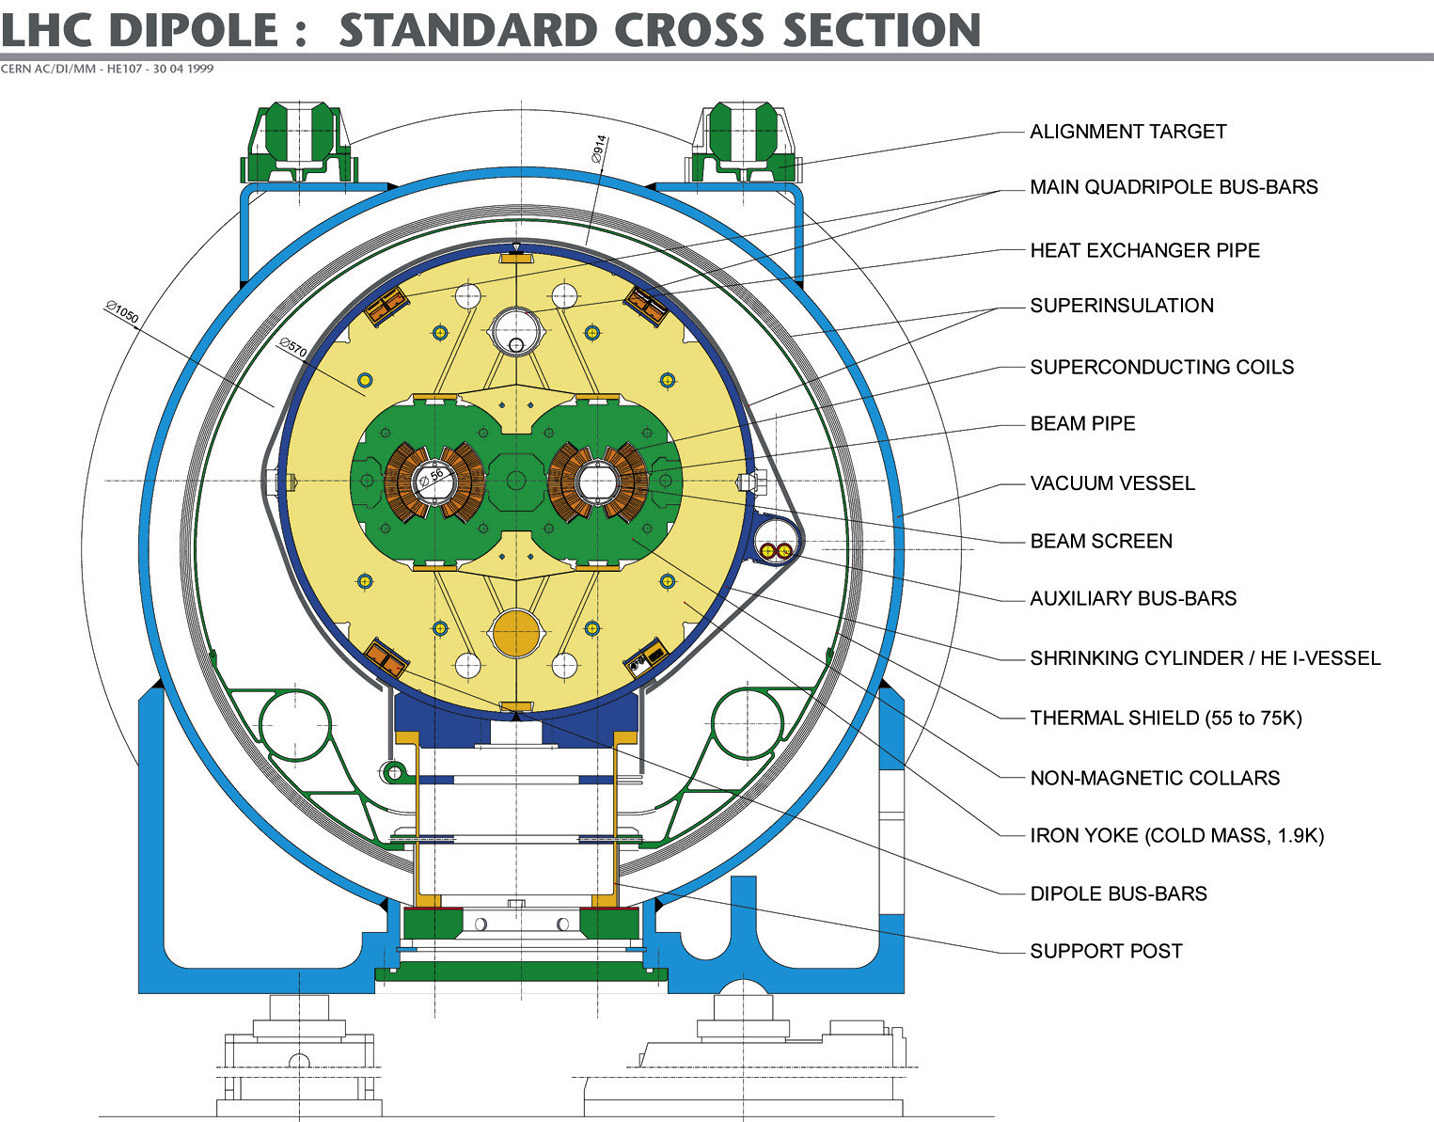
\includegraphics[width=0.7\textwidth]{lhcdipole}
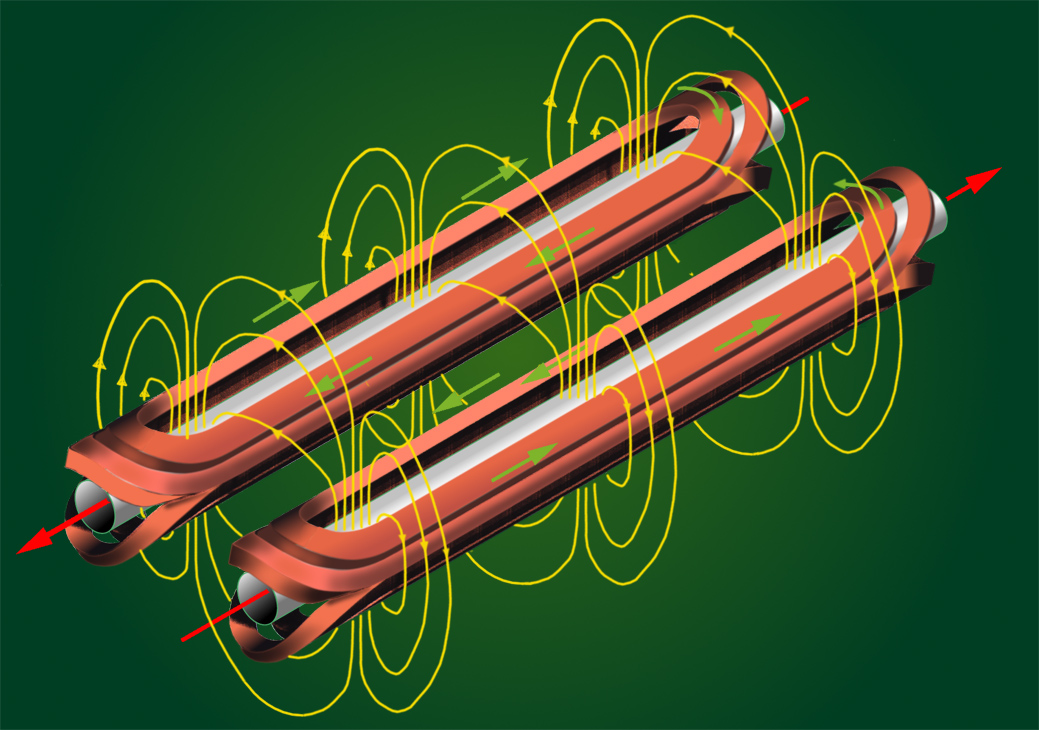
\includegraphics[width=6.0cm,height=4cm]{lhc_dipole2}
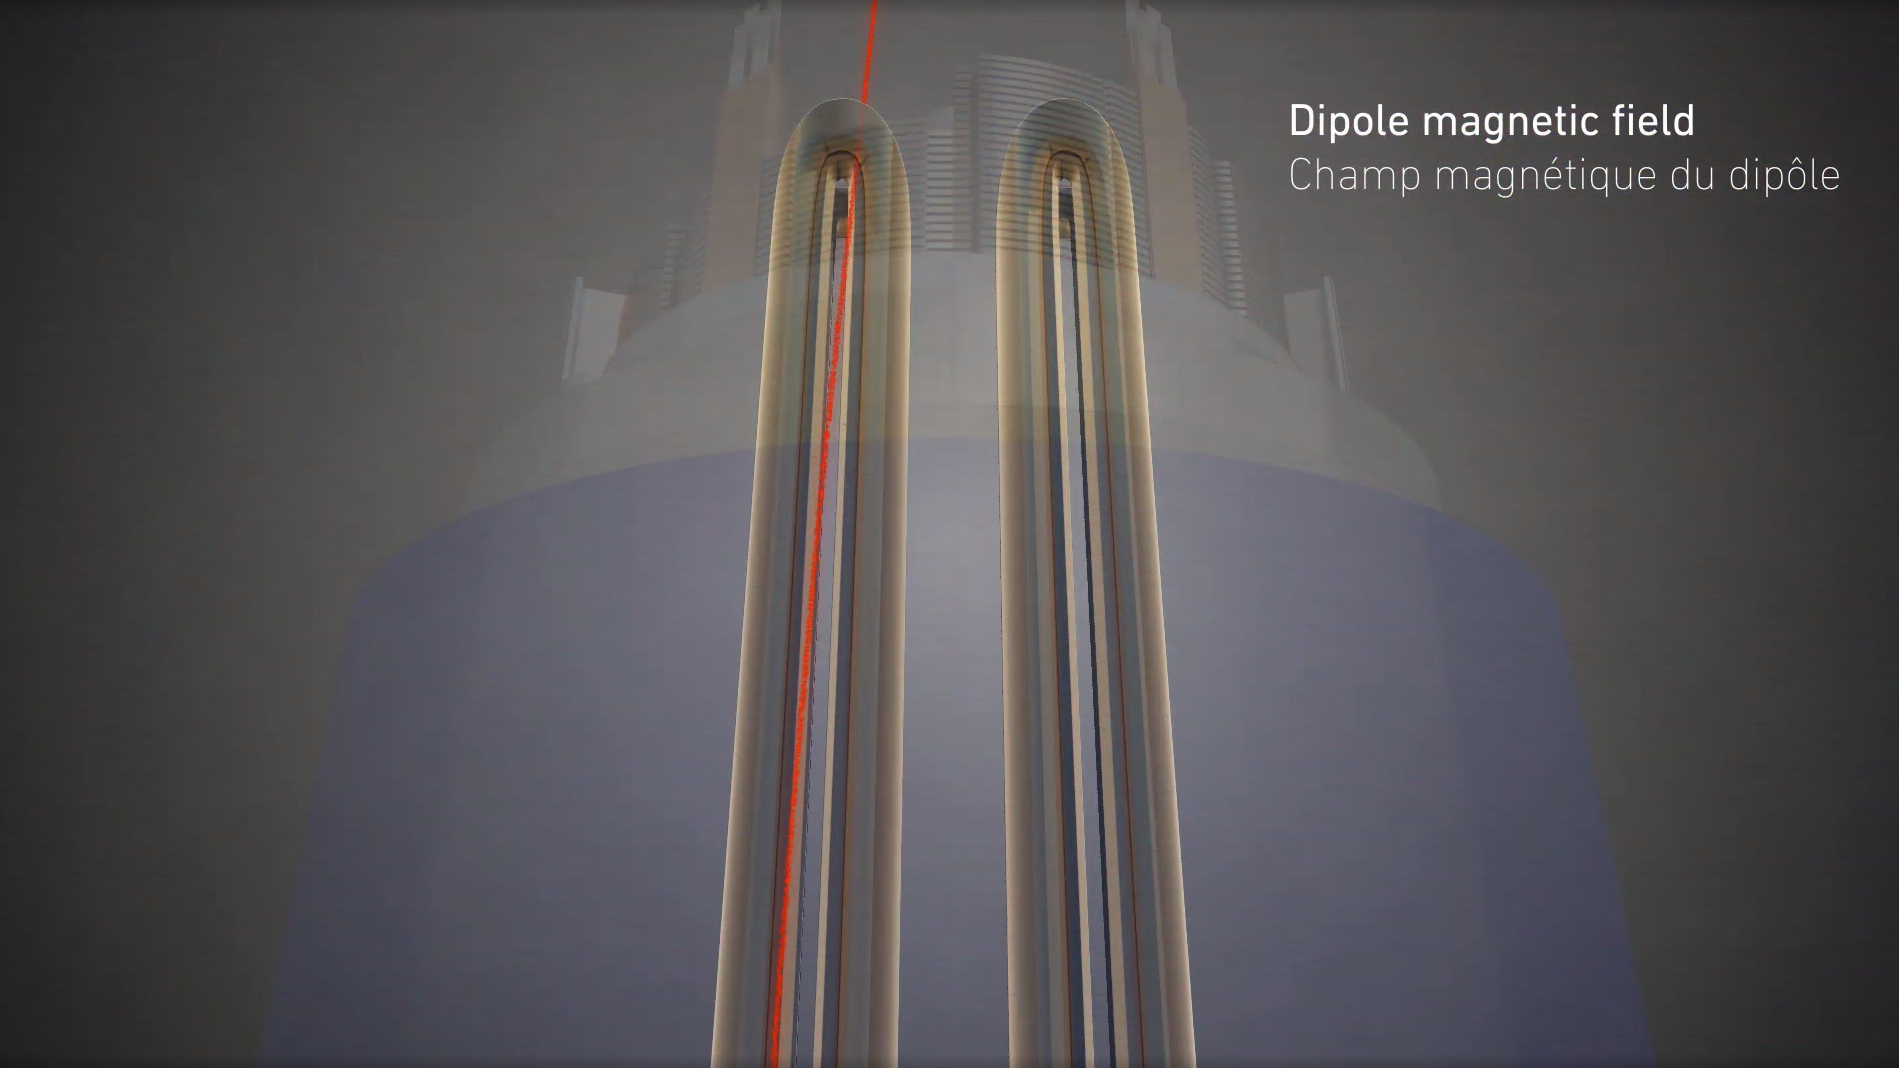
\includegraphics[width=6.0cm,height=4cm]{beam_dev}
\caption [LHC dipole magnet.]{Top: LHC dipole magnet transverse view; cooling, shielding and mechanical support are indicated. Bottom left: Magnetic field generated by the dipole magnets; note that the direction of the field inside one beam pipe is opposite with respect to the other beam pipe which guarantee that both proton beams are curved in the same direction towards the center of the ring. The effect of the dipole magnetic field on the proton beam is represented on the bottom right side \cite{lhc_dipole, dipole_field,video}.}\label{fig:lhcdipole}
\end{figure}

Protons in the arc sections of LHC feel a centripetal force exerted by the dipole magnets; the magnitude of magnetic field needed to keep the protons in the LHC curved trayectory can be found by considering the Loretz force
\beqn
\frac{d\textbf{p}}{dt}= q\textbf{v}\times \textbf{B}.
\eeqn

Solving for \textbf{p}, it is found that

\beqn
\frac{p}{q}=Br 
\eeqn

\noindent where p is the proton's momentum (7 TeV/c), q is the proton's charge and r is the LHC radius, thus, B=8.33 T which is about 100000 times the Earth's magnetic field. A representation of the magnetic field generated by the dipole magnets is shown on the bottom left side of Figure \ref{fig:lhcdipole}. The bending effect of the magnetic field on the proton beam is shown on the bottom right side of Figure \ref{fig:lhcdipole}. Note that the dipole magnets are not curved; the arc section of the LHC ring is composed of straight dipole magnets of about ${15 \textrm{ m}}$. In total there are 1232 dipole magnets along the LHC ring.

In addition to the bending of the beam trajectory, the beam has to be focused. The focusing is performed by quadrupole magnets installed in a different straight section; in total 858 quadrupole magnets are installed along the LHC ring. Other effects like electromagnetic interaction among bunches, interaction with electron clouds from the beam pipe, the gravitational force on the protons, differences in energy among protons in the same bunch, among others, are corrected using sextupole and other magnetic multipoles.

The two proton beams inside the LHC ring are made of bunches with a cylindrical shape of about 7.5 cm long and about 1 mm in diameter; when bunches are close to the interaction point (IP), the beam is focused up to a diameter of about 16 $\mu$m in order to maximize the probability of collisions between protons. The number of collisions per second is proportional to the cross section of the bunches with the \ti{luminosity} (L) as the proportionality factor, thus, the luminosity can be calculated using

\beqn
L=fn\frac{N_1 N_2}{4\pi \sigma_x\sigma_y}\label{eq:lumi}
\eeqn

\noindent where f is the revolution frequency, n is the number of bunches per beam, $N_1$ and $N_2$ are the numbers of protons per bunch, $\sigma_x$ and $\sigma_y$ are the gaussian transverse sizes of the bunches. With the expected parameters, the LHC expected luminosity is about  

\begin{align}
  f=&\frac{v}{2\pi r_{LHC}}\approx\frac{3\times10^8\textrm{m/s}}{27\textrm{km}}\approx 11.1 \textrm{kHz},\nonumber \\
  n=&2808\nonumber \\ 
  N_1=&N_2 \sim1.5\times 10^{11}\nonumber\\
  \sigma_x=&\sigma_y=16\mu \textrm{m}\nonumber
\end{align}
\beqn
L= 1.28\times 10^{34} \textrm{cm}^{-2}\textrm{s}^{-1} = 1.28 \times 10^{-5} \textrm{fb}^{-1}\textrm{s}^{-1}
\eeqn

\noindent where 1 barn (b) corresponds to $10^{-28}$ m$^2$, hence, 1 fb = 10$^{-39}$ cm$^2$. 

\begin{figure}[!h]
\centering
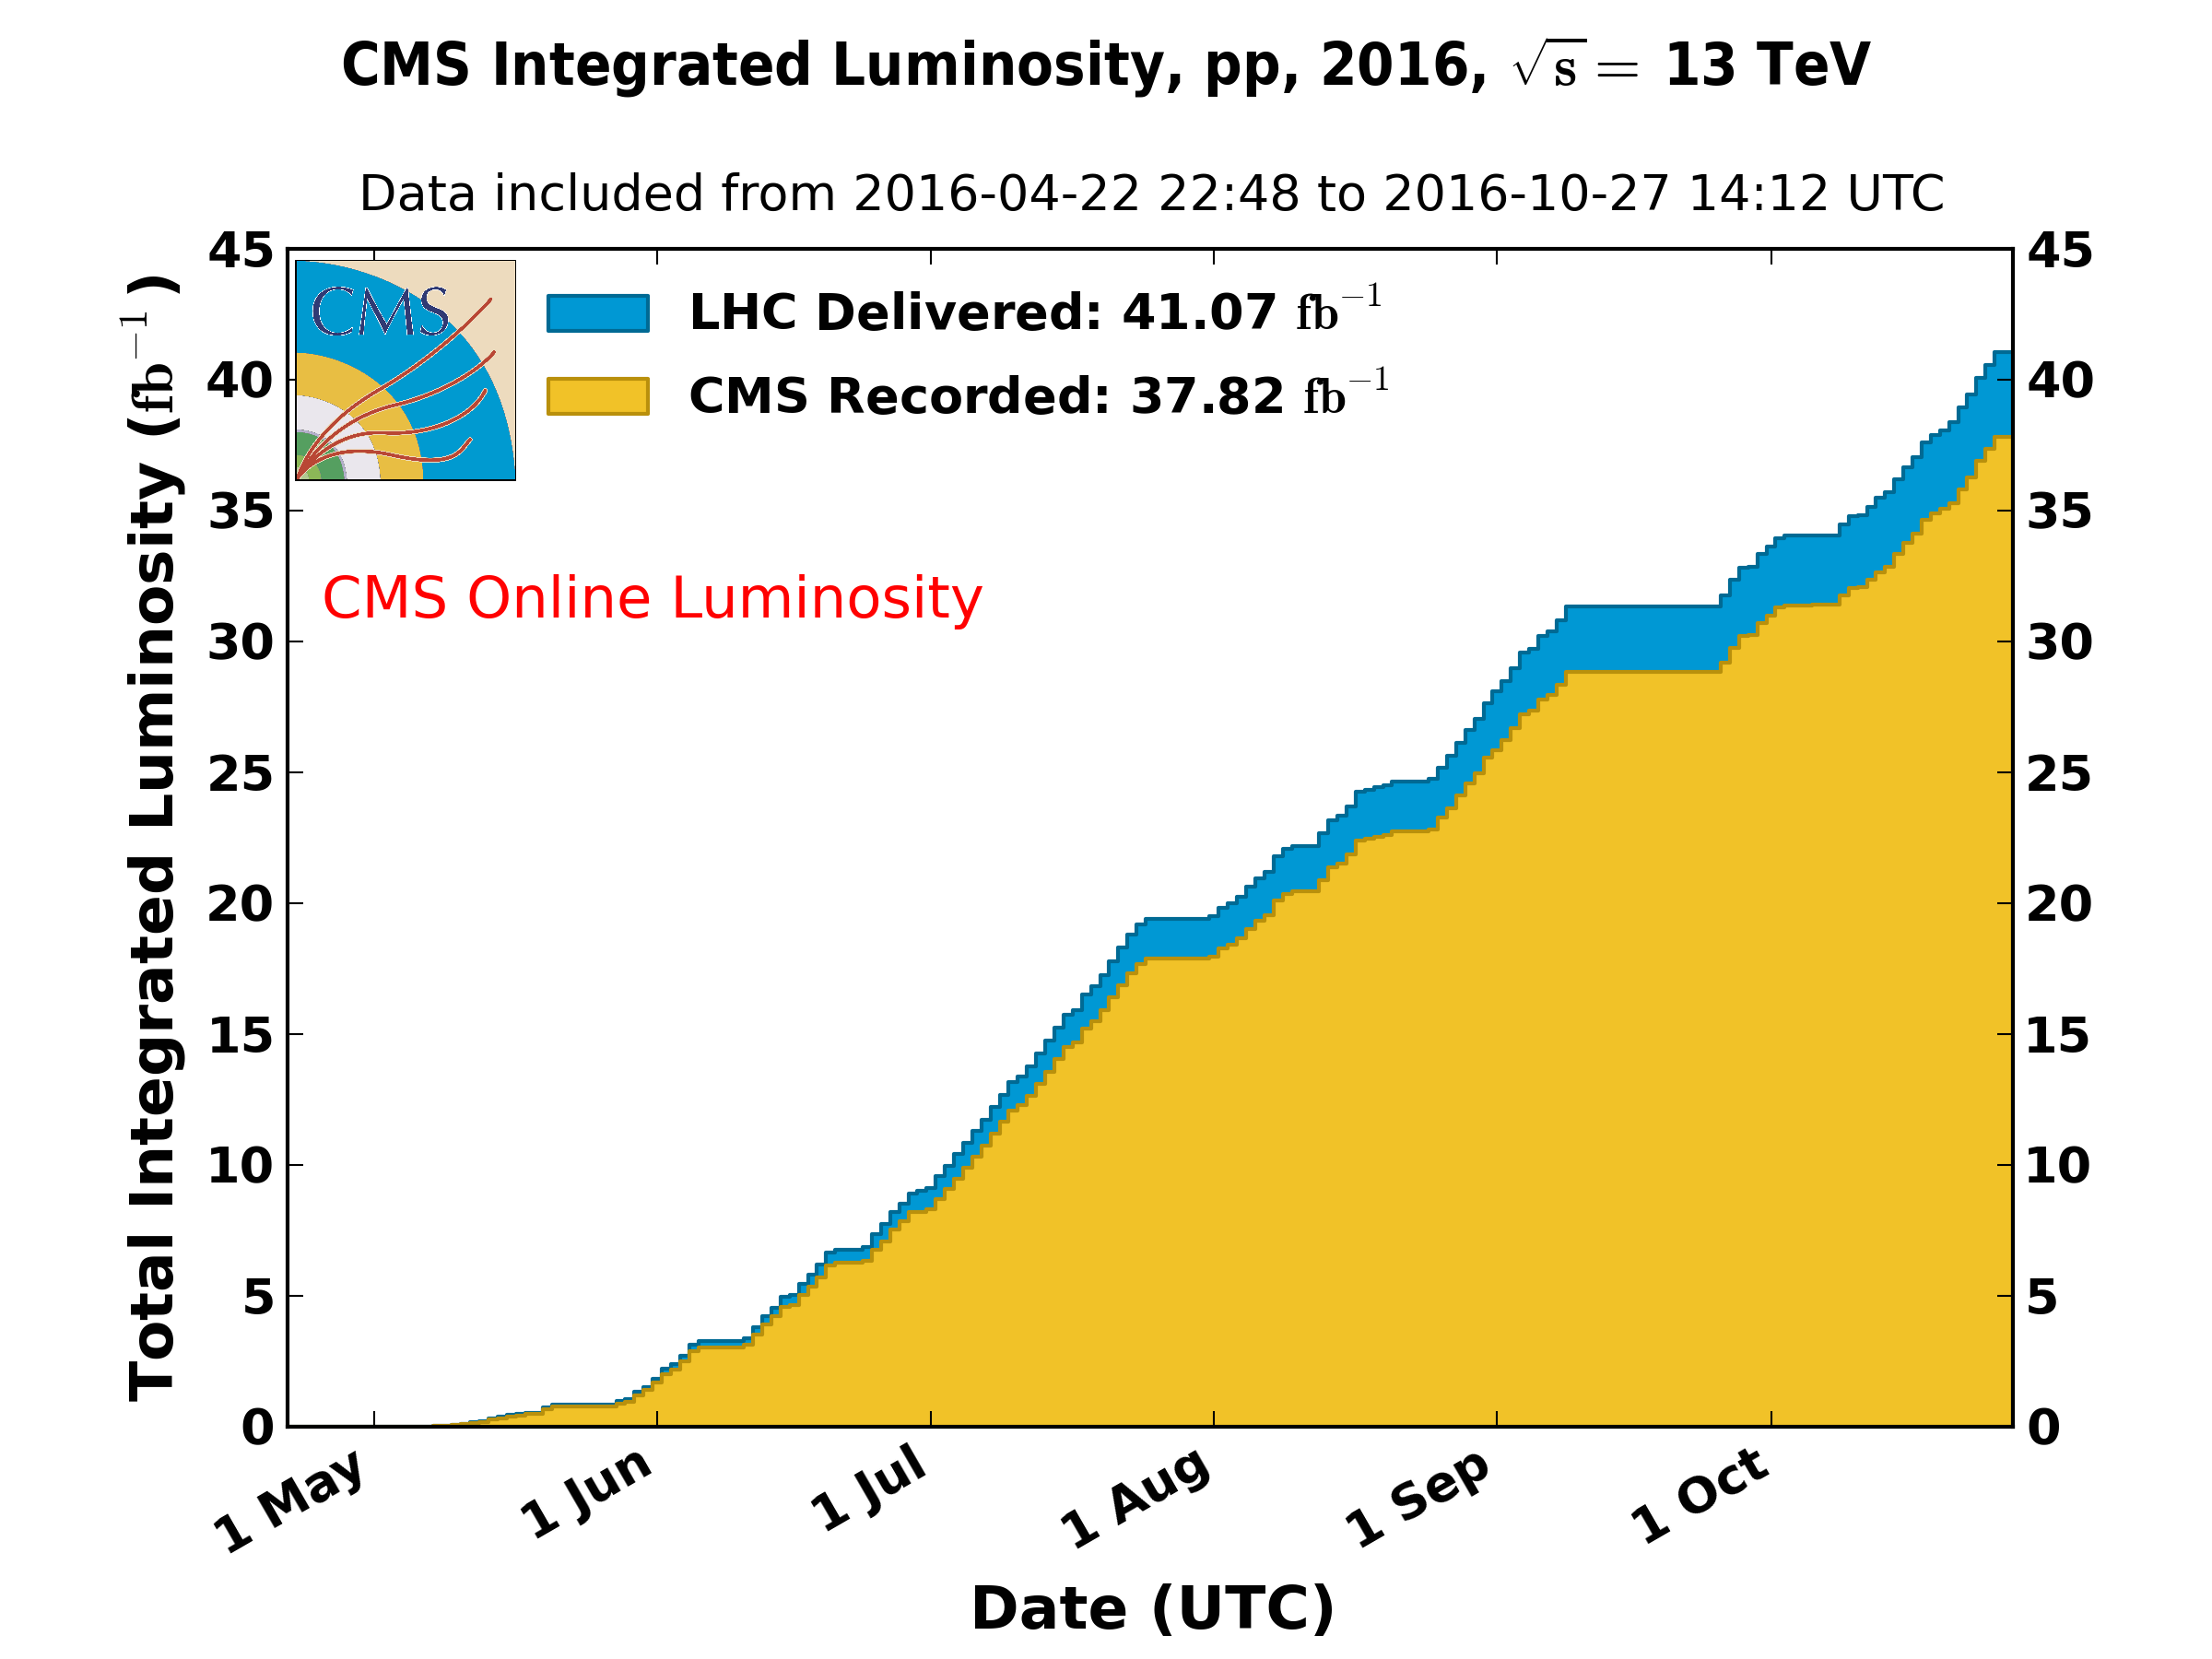
\includegraphics[width=0.7\textwidth]{int_lumi_2016_cms}
\caption [Integrated luminosity delivered by LHC and recorded by CMS during 2016]{Integrated luminosity delivered by LHC and recorded by CMS during 2016. The difference between the delivered and the recorded luminosity is due to fails and issues occurred during the data taking in the CMS experiment \cite{lumi}.}\label{fig:lumi}
\end{figure}

Luminosity is a fundamental aspect of LHC given that the bigger luminosity the bigger number of collisions, which means that for processes with a very small cross section the number of expected occurrences is increased and so the chances of being detected. The integrated luminosity, collected by the CMS experiment during 2016 is shown in Figure \ref{fig:lumi}; the data analyzed in this thesis corresponds to an integrated luminosity of 35.9 fb$^{-1}$ at a center of mass-energy $\sqrt{s}=13$ TeV. 

One way to increase L is increasing the number of bunches in the beam. Currently, the separation between two consecutive bunches in the beam is 7.5 m which corresponds to a time separation of 25 ns. In the full LHC ring the allowed number of bunches is $n=27\textrm{ km}/7.5\textrm{ m}=3600$; however, there are some gaps in the bunch pattern intended for preparing the dumping and injection of the beam, thus, the proton beams are composed of 2808 bunches.

Once the proton beams reach the desired energy, they are brought to cross each other producing \pp collisions. The bunch crossing happens in precise places where the four LHC experiments are located, as seen in the top of Figure \ref{fig:lhc_layout}. In 2008 \pp collisions of $\sqrt{s}=7$ TeV were performed; the energy was increased to 8 TeV in 2012 and to 13 TeV in 2015.

\begin{figure}[!h]
\centering
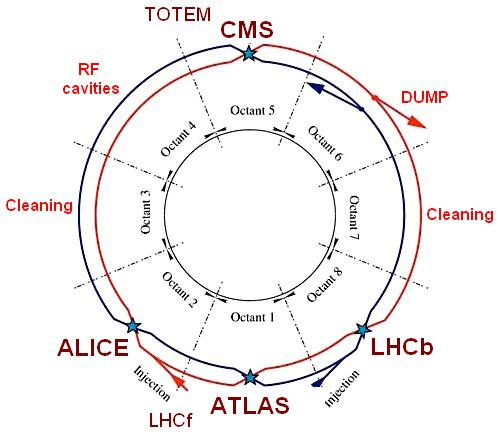
\includegraphics[width=0.55\textwidth]{lhc_layout}
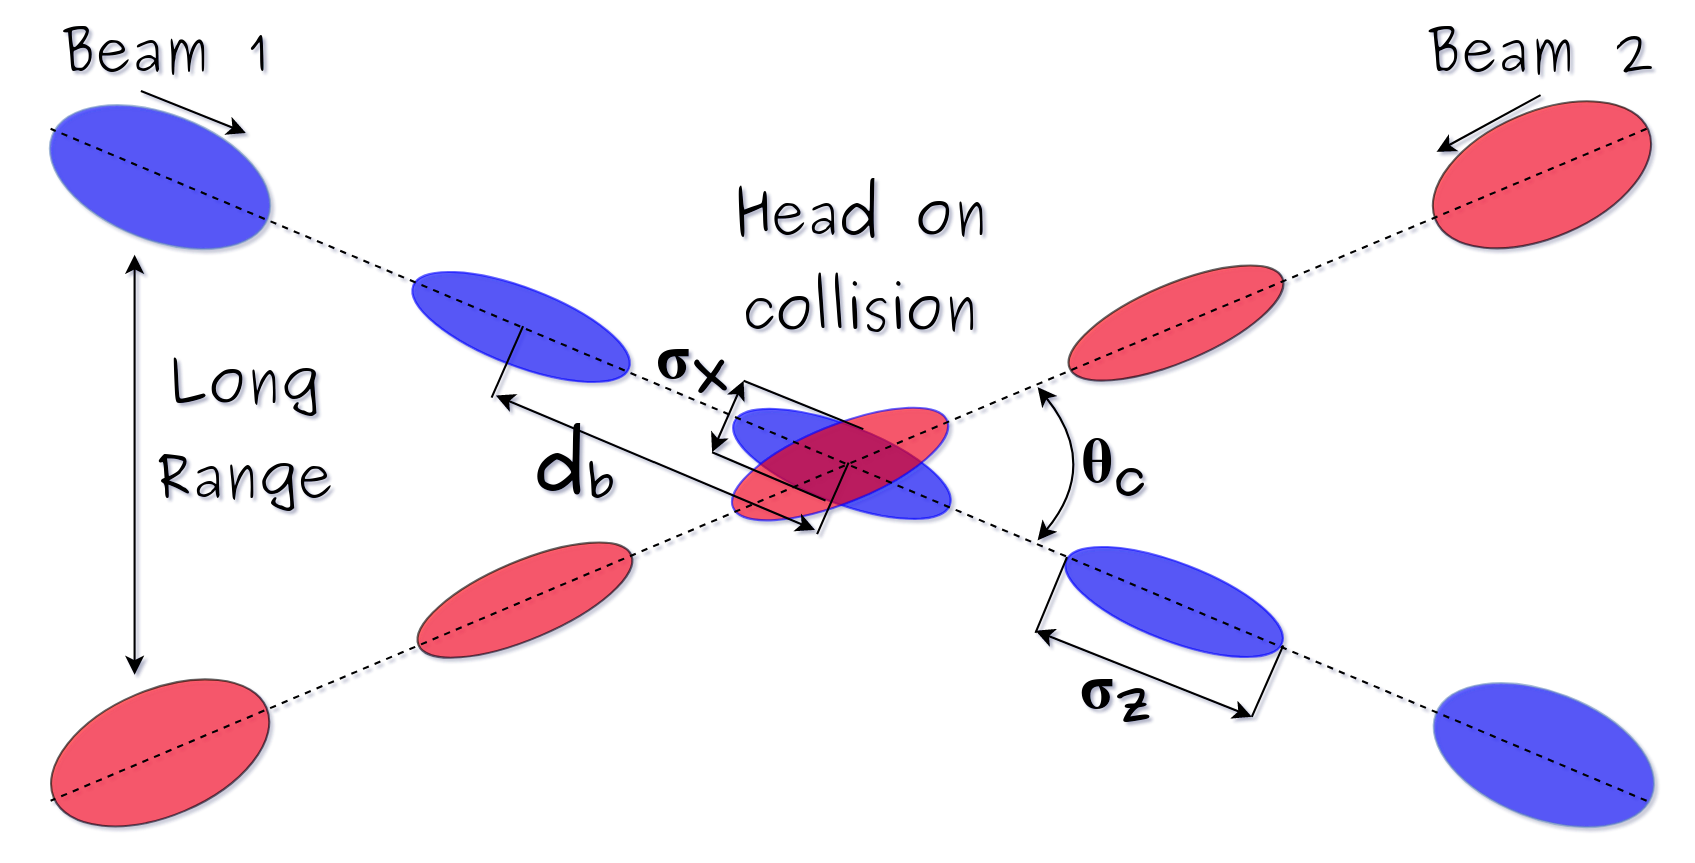
\includegraphics[width=0.6\textwidth]{bcross}
\caption [LHC interaction points]{Top: LHC interaction points. Bunch crossing occurs where the LHC experiments are located \cite{lhc_layout}. Sections indicated as cleaning are dedicated to collimate the beam in order to protect the LHC ring from collisions with protons in very spreaded bunches. Bottom: bunch crossing scheme. Since the bunch crossing is not perfectly head-on, the luminosity is reduced in a factor of 17\%; adapted from Reference \cite{l1}.}\label{fig:lhc_layout}
\end{figure}

The CMS and ATLAS experiments are multi-purpose experiments, hence, they are enabled to explore physics in any of the LHC collision modes. LHCb experiment is optimized to explore bottom quark physics, while ALICE is optimized for heavy ion collisions searches; TOTEM and LHCf are dedicated to forward physics studies; MoEDAL (not indicated in the Figure) is intended for monopole or massive pseudo stable particles searches.

At the IP there are two interesting details that need to be addressed. The first one is that the bunch crossing does not occur head-on but at a small crossing angle \ti{$\theta_c$} (280 $\mu$rad in CMS and ATLAS) as shown in the bottom side of Figure \ref{fig:lhc_layout}, affecting the overlapping between bunches; the consequence is a reduction of about 17\% in the luminosity (represented by a factor not included in eqn. \ref{eq:lumi}). The second one is the occurrence of multiple \pp collisions in the same bunch crossing; this effect is called \ti{pileup} (PU). A fairly simple estimation of the PU follows from estimating the probability of collision between two protons, one from each of the bunches in the course of collision; it depends roughly on the ratio of proton size and the cross section of the bunch in the IP, \ie,
\beqn
P(pp-collision) \sim \frac{d_{proton}^2}{\sigma_x\sigma_y}=\frac{(1 \textrm{fm})^2}{(16\mu \textrm{m})^2} \sim 4\times10^{-21}
\eeqn
\noindent however, there are $N=1.15\times 10^{11}$ protons in a bunch, thus the estimated number of collisions in a bunch crossing is

\beqn
PU= N^2*P(pp-collision)\sim 50  \textrm{\pp collision per bunch crossing},
\eeqn

\noindent about 20 of which are inelastic. %Each collision generates a vertex which corresponds to the position where the interaction actually happened, but only the most energetic is considered as a primary vertex, the rest are considered as PU vertices; more details on how the reconstruction and identification of the vertices is made will be given in Chapter \ref{gensimreco}.
A multiple \pp collision event in a bunch crossing at CMS is shown in Figure \ref{fig:pu}. %Unstable particles outgoing from the primary vertex will eventually decay; this decay vertex is known as a secondary vertex.      

\begin{figure}[!h]
\centering
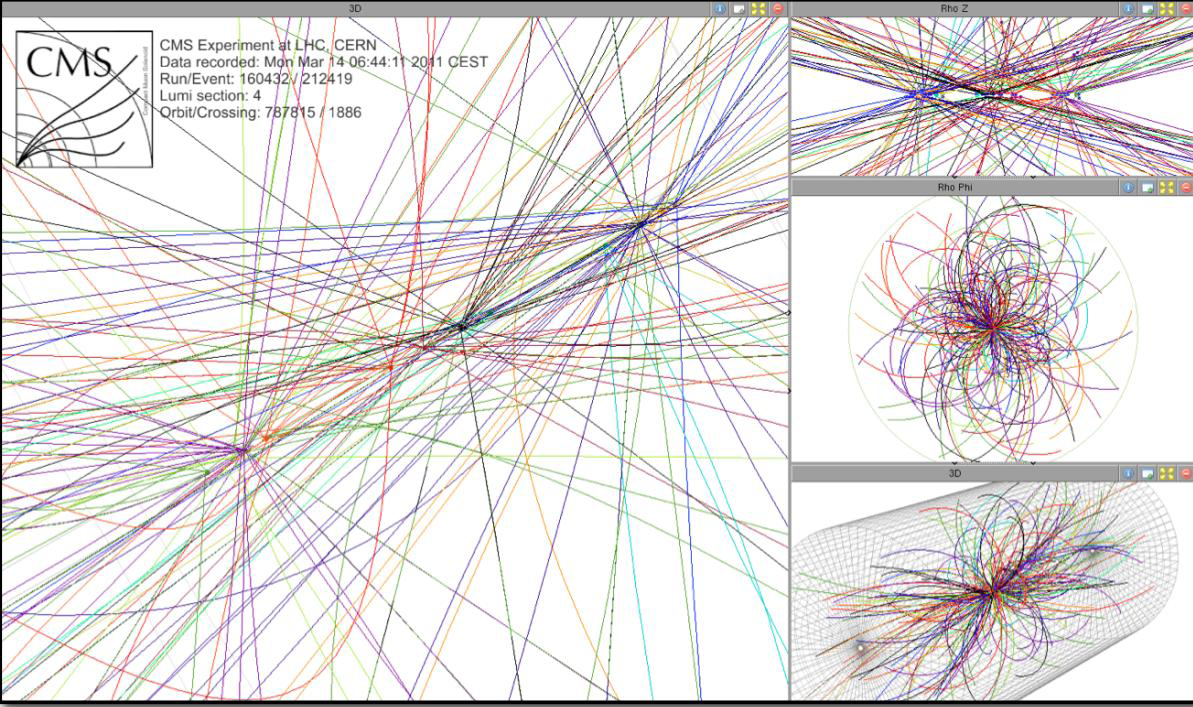
\includegraphics[width=0.65\textwidth]{pu}
\caption [Multiple \pp collision bunch crossing at CMS.]{Multiple \pp collision bunch crossing at CMS. %Only the most energetic vertex is considered and the rest are cataloged as PU vertices
\cite{pu}. }\label{fig:pu}
\end{figure}

\section{The CMS experiment}

CMS is a general-purpose detector designed to conduct research in a wide range of physics from the standard model to new physics like extra dimensions and dark matter. Located at Point 5 in the LHC layout as shown in Figure \ref{fig:lep_rfc}, CMS is composed of several detection systems distributed in a cylindrical structure; in total, CMS weights about 12500 tons in a very compact 21.6 m long and 14.6 m diameter cylinder. It was built in 15 separate sections at the ground level and lowered to the cavern individually to be assembled. A complete and detailed description of the CMS detector and its components is given in Reference \cite{cms} on which this section is based.

\noindent Figure \ref{fig:cms} shows the layout of the CMS detector. The detection system is composed of (from the innermost to the outermost)

\begin{figure}[!h]
  \centering
  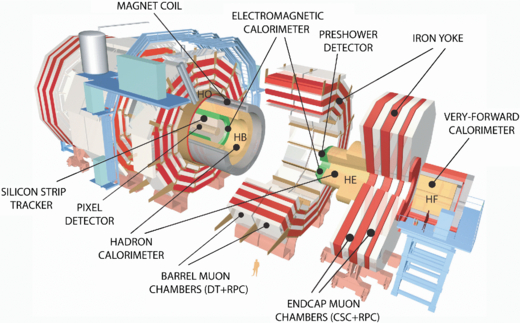
\includegraphics[width=\textwidth]{cms}
  \caption[Layout of the CMS detector]{Layout of the CMS detector. The several subdetectors are indicated. The central region of the detector is referred as the barrel section while the endcaps are referred as the forward sections. \cite{cms_drawing}.}
  \label{fig:cms}
\end{figure}

\bit
\item Pixel detector.
\item Silicon strip tracker.
\item Preshower detector.
\item Electromagnetic calorimeter.
\item Hadronic calorimeter.
\item Muon chambers (barrel and endcap)
\eit

The central region of the detector is commonly referred as the barrel section while the endcaps are referred as the forward sections of the detector; thus, each subdetector is composed of a barrel section and a forward section. 

When a \pp collision happens inside the CMS detector, many different particles are produced, but only some of them live long enough to be detected; they are electrons, photons, pions, kaons, protons, neutrons and muons; neutrinos are not detected by the CMS detector. Thus, the CMS detector was designed to detect those particles and measure their properties. Figure \ref{fig:cms_slice} shows a transverse slice of the CMS detector. The silicon tracker (pixel detector + strip tracker) is capable to register the track of the charged particles traversing it, while calorimeters (electromagnetic and hadronic) measure the energy of the particles that are absorbed by their materials. Considering the detectable particles, mentioned above, emerging from the IP, a basic description of the detection process is as follows. 

\begin{figure}[h!]
  \centering
  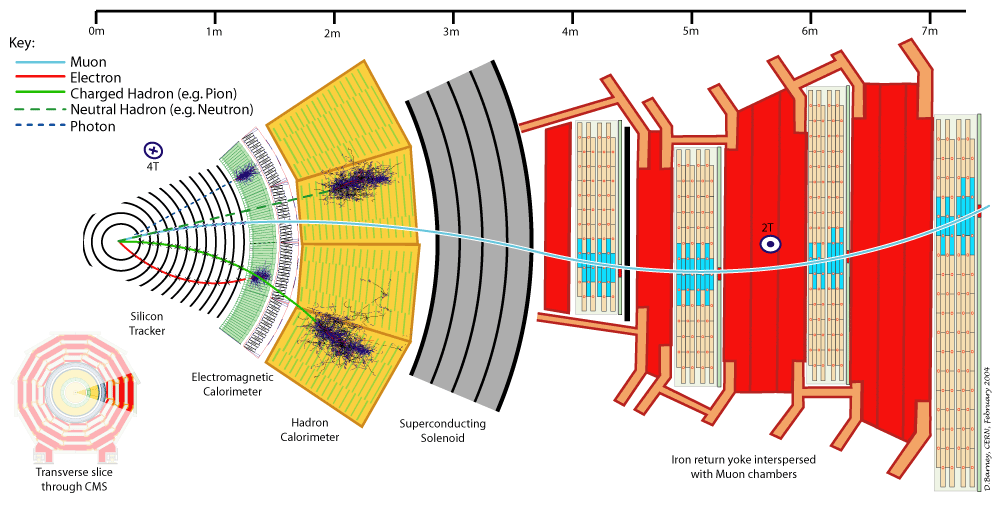
\includegraphics[width=\textwidth]{cms_slice}
  \caption[CMS detector transverse slice]{CMS detector transverse slice \cite{cms_slice}.}
  \label{fig:cms_slice}
\end{figure}

A muon emerging from the IP, will create a track on the silicon tracker and on the muon chambers. The design of the CMS detector is driven by the requirements on the identification, momentum resolution and unambiguous charge determination of the muons; therefore, a large bending power is provided by the solenoid magnet made of superconducting cable capable of generating a 3.8 T magnetic field. The muon track is bent twice since the magnetic field inside the solenoid is directed along the $z$-direction but outside its direction is reversed. Muons interact very weakly with the calorimeters, therefore, it is not absorbed but escape away from the detector.  

An electron emerging from the IP will create a track along the tracker which will be bent due to the presence of the magnetic field, later, it will be absorbed in the electromagnetic calorimeter where its energy is measured.

A photon will not leave a track because it is neutral, but it will be absorbed in the electromagnetic calorimeter.

A neutral hadron, like the neutron, will not leave a track either but it will lose a small amount of its energy during its passage through the electromagnetic calorimeter and then it will be absorbed in the hadron calorimeter depositing the rest of its energy.

A charged hadron, like the proton or $\pi^\pm$, will leave a curved track on the silicon tracker, some of its energy in the electromagnetic calorimeter and finally will be absorbed in the hadronic calorimeter.

A more detailed description of each detection system will be presented in the following sections. 

\subsection{CMS coordinate system}

The coordinate system used by CMS is centered on the geometrical center of the detector which is the nominal IP as shown in Figure \ref{fig:coord}\footnote{Not all the \pp interaction occur at the nominal IP because of the bunch lenght, therefore, each \pp collision has it own IP location}. The $z$-axis is parallel to the beam direction, while the $Y$-axis pointing vertically upward, and the $X$-axis pointing radially inward toward the center of the LHC.

\begin{figure}[h!]
  \centering
  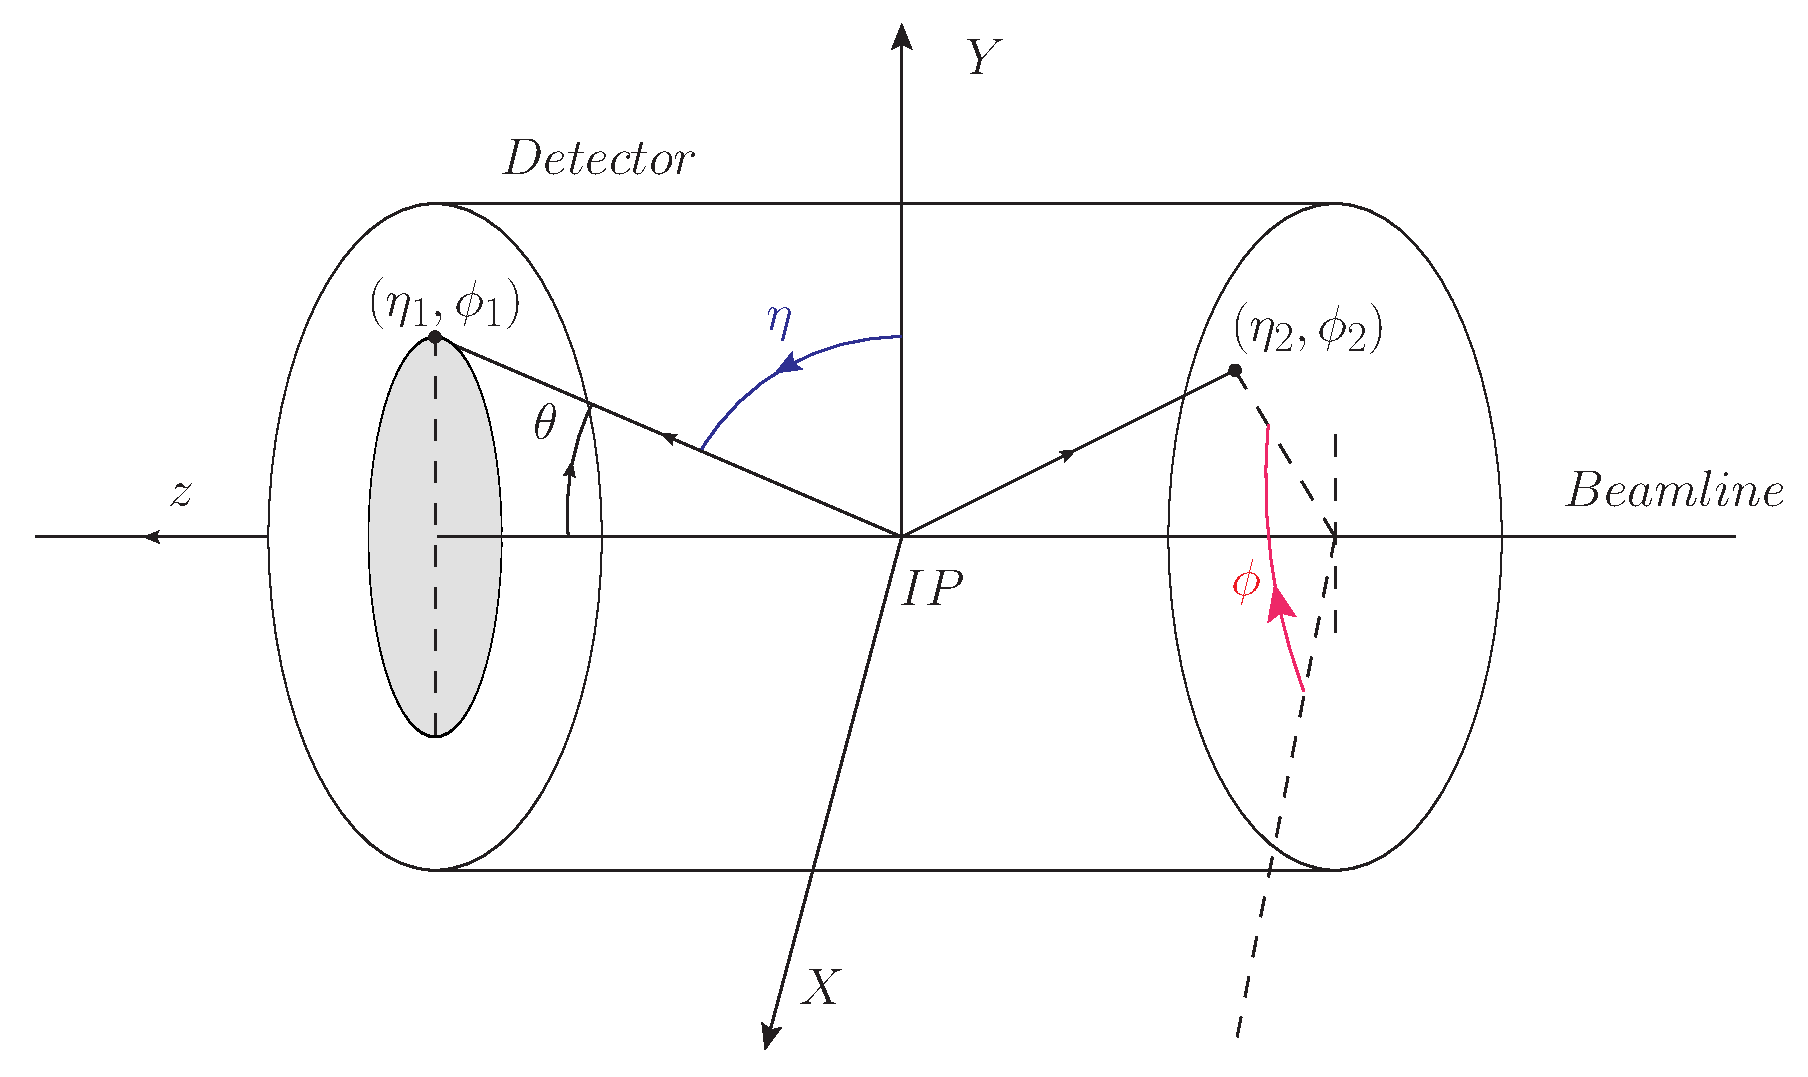
\includegraphics[scale=0.4]{coord}
  \caption[CMS detector coordinate system]{CMS detector coordinate system.}
  \label{fig:coord}
\end{figure}

In addition to the common cartesian and cylindrical coordinate systems, two coordinates are of particular utility in particle physics: rapidity ($y$) and pseudorapidity ($\eta$), defined in connection to the polar angle $\theta$, energy and longitudinal momentum component (momentum along the $z$-axis) according to

\beqn
y=\frac{1}{2}ln\frac{E+p_z}{E-p_z} \qquad \eta=-ln \left(tan\frac{\theta}{2}\right)
\label{eqn:eta}
\eeqn

Rapidity is related to the angle between the $XY$-plane and the direction in which the products of a collision are emitted; it has the nice property that the difference between the rapidities of two particles is invariant with respect to Lorentz boosts along the $z$-axis, hence, data analysis becomes more simple when based on rapidity; however, it is not simple to measure the rapidity of highly relativistic particles, as those produced after \pp collisions. Under the highly relativistic motion approximation, $y$ can be rewritten in terms of the polar angle, concluding that rapidity is approximately equal to the pseudorapidity defined above, \ie, $y\approx\eta$. Note that $\eta$ is easier to measure that $y$ given the direct relationship between the former and the polar angle.

The angular distance between two objects in the detector ($\Delta R$) is commonly used to judge the isolation of those object; it is defined in terms of their coordinates $(\eta_1,\phi_1)$, $(\eta_2,\phi_2)$ as
\beqn
\Delta R = \sqrt{(\Delta\eta)^2 - (\Delta\phi)^2 }
\label{delta_r}
\eeqn

\subsection{Tracking system}

The CMS tracking system is designed to provide a precise measurement of the trajectories (\textit{track}) followed by the charged particles created after the \pp collisions; also, the precise reconstruction of the primary and secondary origins of the tracks (\textit{vertices}) is expected in an environment where, each 25 ns, the bunch crossing produces about 20 inelastic collisions and about 1000 particles.% An increment in the luminosity is ongoing which implies that the PU will increase accordingly.

Physics requirements guiding the tracking system performance include the precise characterization of events involving gauge bosons, W and Z, and their leptonic decays for which an efficient isolated lepton and photon reconstruction is of capital importance, given that isolation is required to suppress background events to a level that allows observations of interesting processes like Higgs boson decays or beyond SM events.

The ability to identify and reconstruct $b$-jets and B-hadrons within these jets is also a fundamental requirement, achieved through the ability to reconstruct accurately displaced vertices, given that $b$-jets are part of the signature of top quark physics, like the one treated in this thesis.

An schematic view of the CMS tracking system is shown in Figure \ref{fig:tracker} 

\begin{figure}[h!]
  \centering
  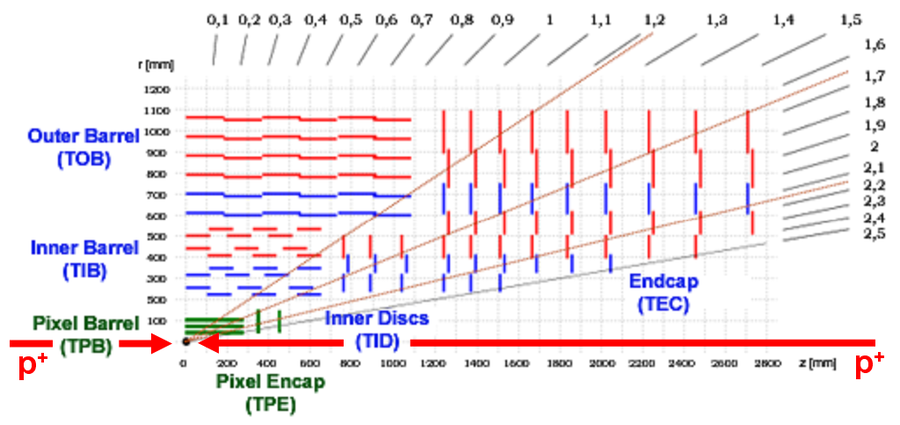
\includegraphics[width=12cm]{tracker}
  \caption[CMS tracking system schematic view.]{CMS tracking system schematic view \cite{tracker}.}
  \label{fig:tracker}
\end{figure}

In order to satisfy these performance requirements, the tracking system uses two different detector subsystems arranged in concentric cylindrical volumes, the pixel detector and the silicon strip tracker; the pixel detector is located in the high particle density region (r<20 cm) while the silicon strip tracker is located in the medium and lower particle density regions 20 cm<r<116 cm.        

\subsubsection*{Pixel detector}


\begin{figure}[h!]
  \centering
  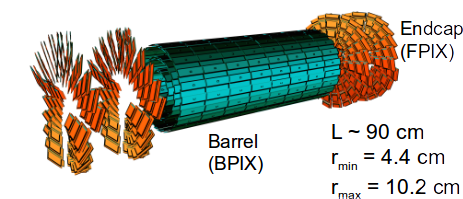
\includegraphics[width=12cm]{pixel}\\
  %\includegraphics[width=6cm]{}
  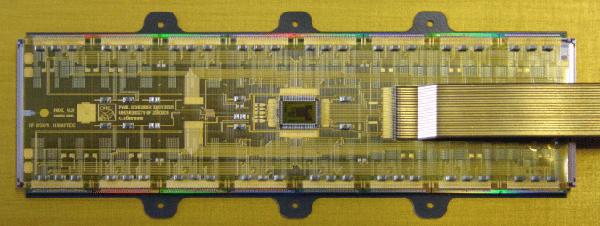
\includegraphics[width=5cm,angle=90]{bpix2}
  \includegraphics[width=7cm,height=5cm]{fpix2}
  \caption[CMS pixel detector]{CMS pixel detector. Top: schematic view; Bottom: pictures of a barrel(BPIX) module(left) and forward modules(right) \cite{cms}.}
  \label{fig:pixel_det}
\end{figure}

The pixel detector was replaced during the 2016-2017 extended year-end technical stop, due to the increasingly challenging operating conditions like the higher particle flux and more radiation harsh environment, among others. The new one is responding as expected, reinforcing its crucial role in the successful way to fulfill the new LHC physics objectives after the discovery of the Higgs boson. Since the data sets used in this thesis were produced using the previous version of the pixel detector, it will be the subject of the description in this section. The last chapter of this thesis is dedicated to describe my contribution to the \ti{ Forward Pixel Phase 1 upgrade}.

The pixel detector was composed of 1440 silicon pixel detector modules organized in three-barrel layers in the central region (BPix) and two disks in the forward region (FPix) as shown in the top side of Figure \ref{fig:pixel_det}; it was designed to record efficiently and with high precision, up to 20 $\mu$m in the $XY$-plane and 20 $\mu$m in the $z$-direction, the first three space-points (\textit{hits}) nearest to the IP region in the range $|\eta|\leq 2.5$. The first barrel layer was located at a radius of 44 mm from the beamline, while the third layer was located at a radius of 102 mm, closer to the strip tracker inner barrel layer (see Section \ref{sst}) in order to reduce the rate of fake tracks. The high granularity of the detector is represented in its about 66 Mpixels, each of size $100\times150 \mu$m$^2$. The transverse momentum resolution of tracks can be measured with a resolution of 1-2\% for muons of $p_T=100$ GeV. 

A charged particle passing through the pixel sensors produce ionization in them, giving energy for electrons to be removed from the silicon atoms, hence, creating electron-hole pairs. The collection of charges in the pixels generates an electrical signal that is read out by an electronic readout chip (ROC); each pixel has its own electronics which amplifies the signal. Combining the signal from the pixels activated by a traversing particle in the several layers of the detector allows one to reconstruct the particle's trajectory in 3D.

Commonly, the charge produced by traversing of a particle is collected by and shared among several pixels; by interpolating between pixels, the spatial resolution is improved. In the barrel section the charge sharing in the r$\phi$-plane is due to the Lorentz effect. In the forward pixels the charge sharing is enhanced by arranging the blades in the turbine-like layout as shown in Figure \ref{fig:pixel_det} bottom left.
%% \begin{figure}[h!]
%%   \centering
%%   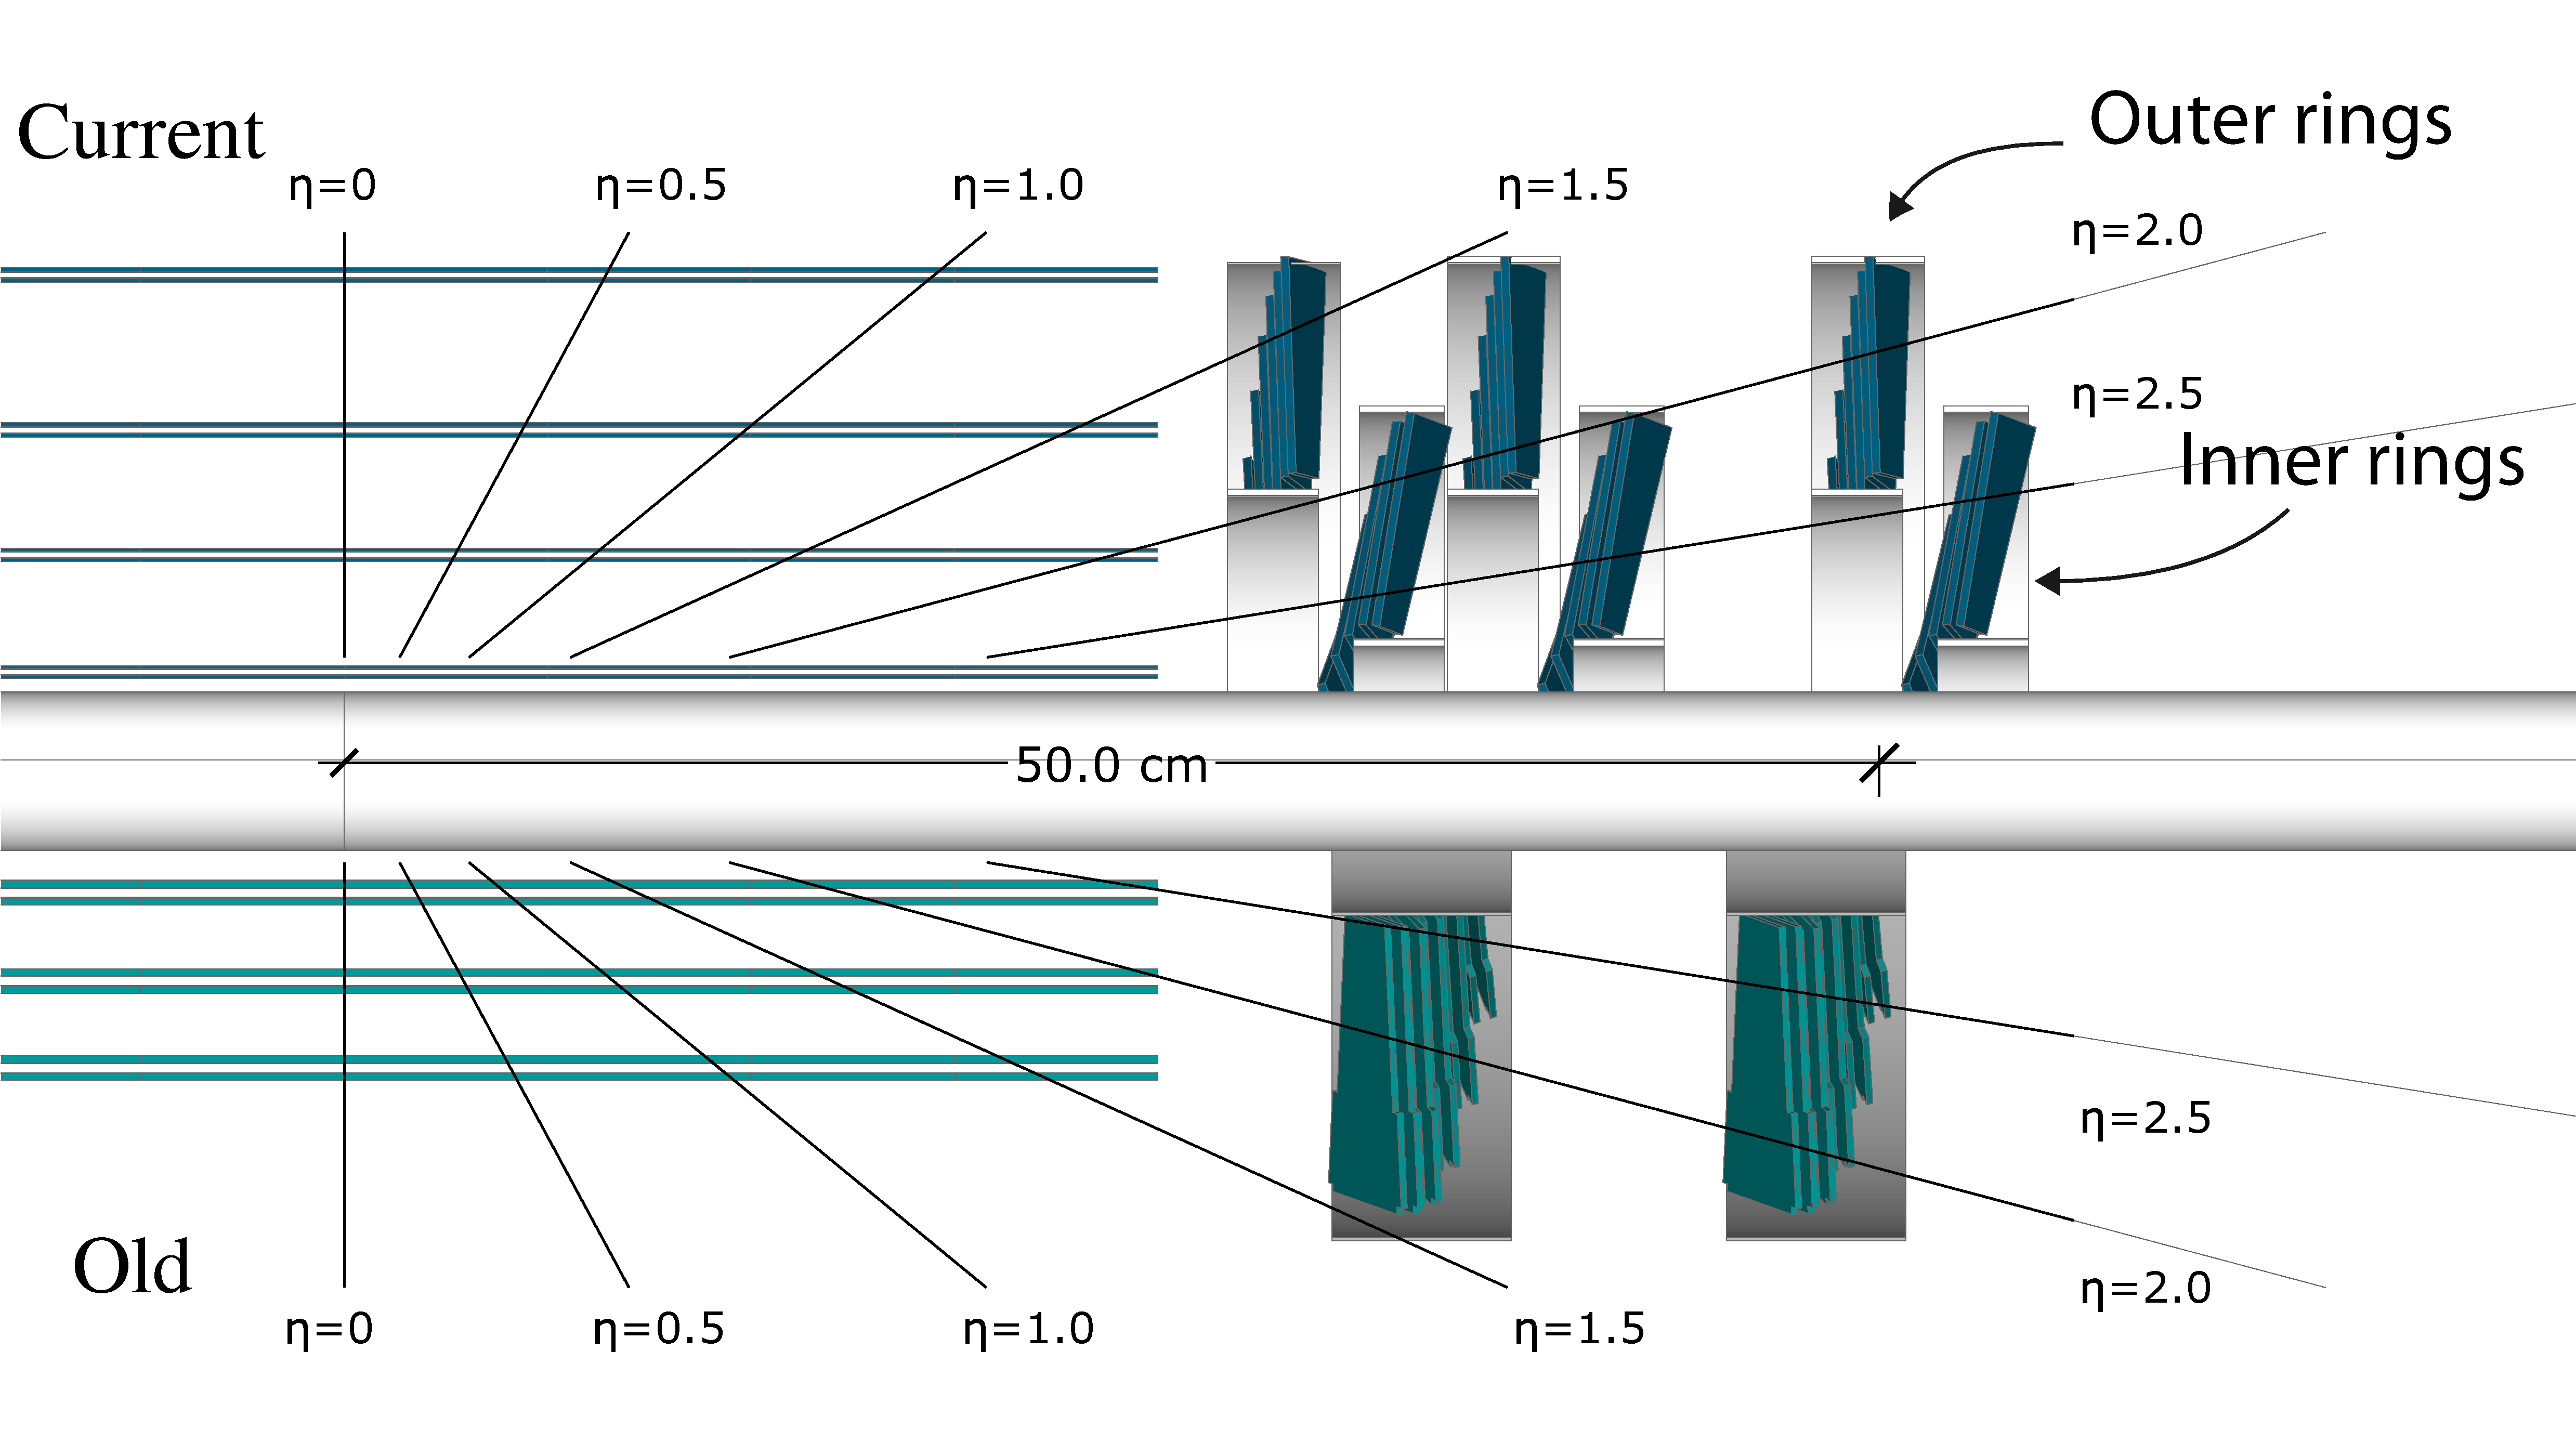
\includegraphics[width=9.5cm]{fpix1}
%%   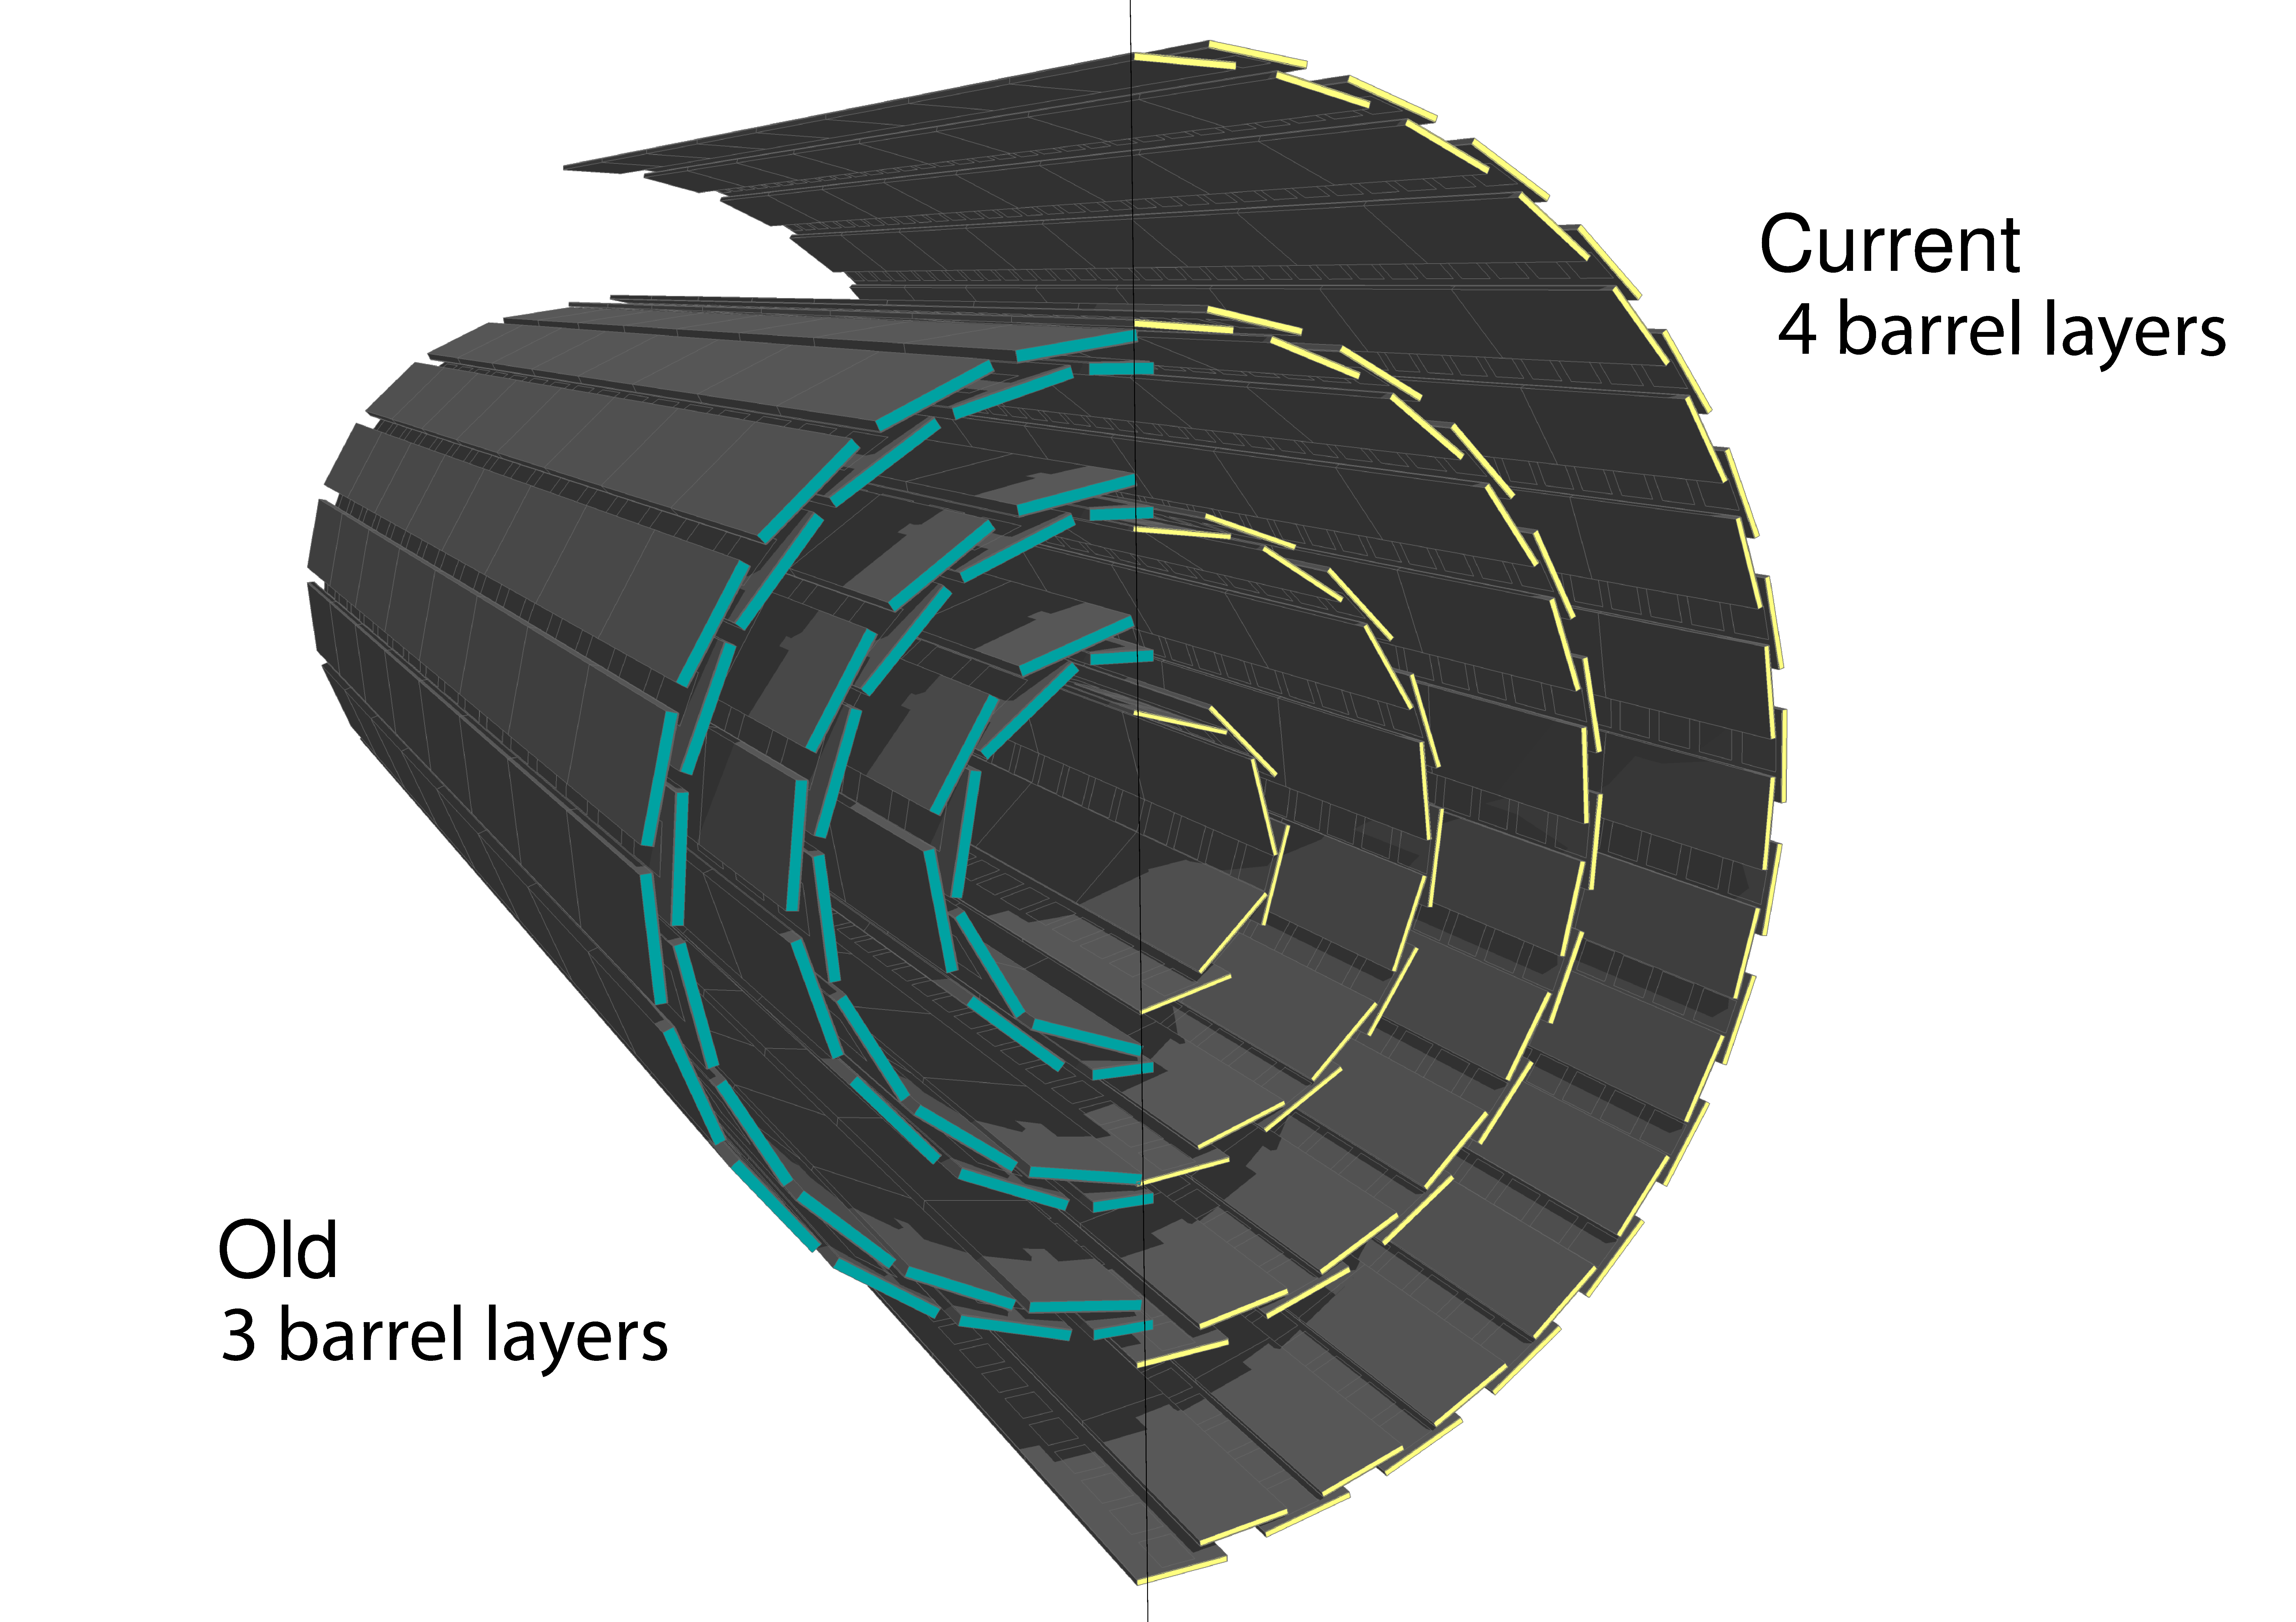
\includegraphics[width=5.5cm]{bpix1}
%%   \caption[CMS pixel detector schematic view.]{CMS pixel detector schematic view. Left: layout comparing the layers and disks in the old and current pixel detectors. Right: Transverse-oblique view comparing the pixel barrel layers in the two \cite{pix_tdr}.}
%%   \label{fig:pixel_tracker}
%% \end{figure}

%% \noindent Some of the improvements with respect to the previous pixel detector include a higher average tracking efficiency and lower average fake rate as well as higher track impact parameter resolution which is fundamental in order to increase the efficiency in the identification of jets originating from b quarks (b-tagging). A significant source of improvement comes from the overall reduction in the material budget of the detector which results in fewer photon conversions and less multiple scattering from charged particles.    

\subsection{Silicon strip tracker}\label{sst}
\begin{figure}[h!]
  \centering
  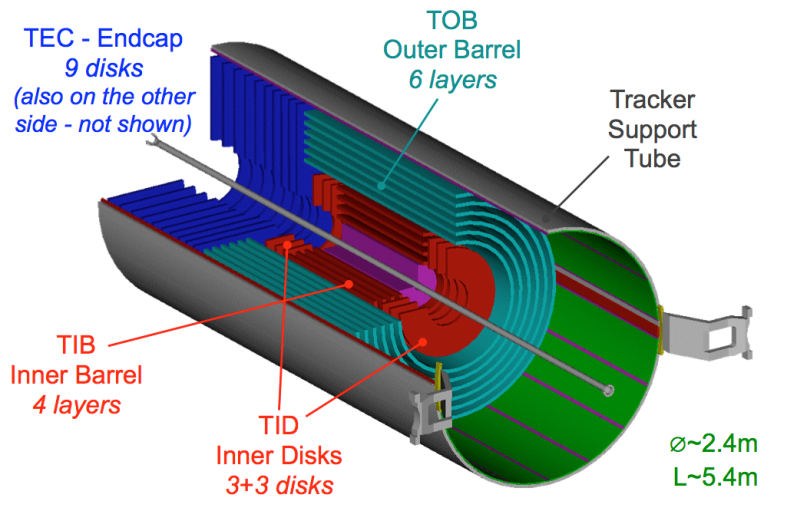
\includegraphics[width=12cm]{sst2}
  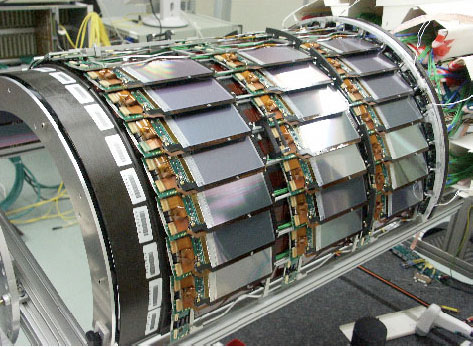
\includegraphics[width=6cm,height=4cm]{tib}
  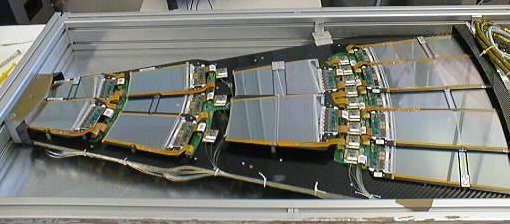
\includegraphics[width=6cm,height=4cm]{tec}
  %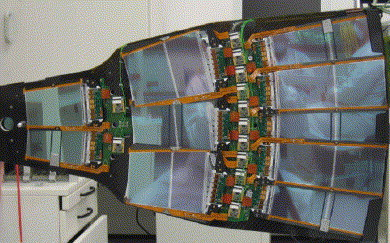
\includegraphics[width=6cm]{tec2}
  \caption[SST Schematic view.]{Top: CMS Silicon Strip Tracker (SST) schematic view. The SST is composed of the tracker inner barrel (TIB), the tracker inner disks (TID), the tracker outer barrel (TOB) and the tracker endcaps (TEC). Each part is made of silicon strip modules; the modules in blue represent two modules mounted back-to-back and rotated in the plane of the module by a stereo angle of 120 mrad in order to provide a 3-D reconstruction of the hit positions. Bottom: pictures of the TIB (left) and TEC (right) modules \cite{sst,tib,tec}.}
  \label{fig:sst}
\end{figure}

The silicon strip tracker (SST) is the second stage in the CMS tracking system. The top side of Figure \ref{fig:sst} shows a schematic of the SST. The inner tracker region is composed of the tracker inner barrel (TIB) and the tracker inner disks (TID) covering the region $r<55$ cm and $|z|<118$ cm. The TIB is composed of 4 layers while the TID is composed of 3 disks at each end. The silicon sensors in the inner tracker are 320 $\mu$m thick, providing a resolution of about 13-38 $\mu$m in the $r\phi$ position measurement.

The modules indicated in blue in the schematic view of Figure \ref{fig:sst} are two modules mounted back-to-back and rotated in the plane of the module by a \ti{stereo} angle of 100 mrad; the hits from these two modules, known as \ti{stereo hits}, are combined to provide a measurement of the second coordinate (z in the barrel and r on the disks) allowing the reconstruction of hit positions in 3-D.

The outer tracker region is composed of the tracker outer barrel (TOB) and the tracker endcaps (TEC). The six layers of the TOB offer coverage in the region $r>55$ cm and $|z|<118$ cm, while the 9 disks of the TEC cover the region $124<|z|<282$ cm. The resolution offered by the outer tracker is about 13-38 $\mu$m in the $r\phi$ position measurement. The inner four TEC disks use silicon sensors 320 $\mu$m thick; those in the TOB and the outer three TEC disks use silicon sensors of 500 $\mu$m thickness. The silicon strips run parallel to the $z$-axis and the distance between strips varies from 80 $\mu$m in the inner TIB layers to 183 $\mu$m in the inner TOB layers; in the endcaps the wedge-shaped sensors with radial strips, whose pitch range between 81 $\mu$m at small radii and 205 $\mu$m at large radii.

The whole SST has 15148 silicon modules, 9.3 million silicon strips and cover a total active area of about 198 m$^2$. 

\subsection{Electromagnetic calorimeter}
\begin{figure}[h!]
  \centering
  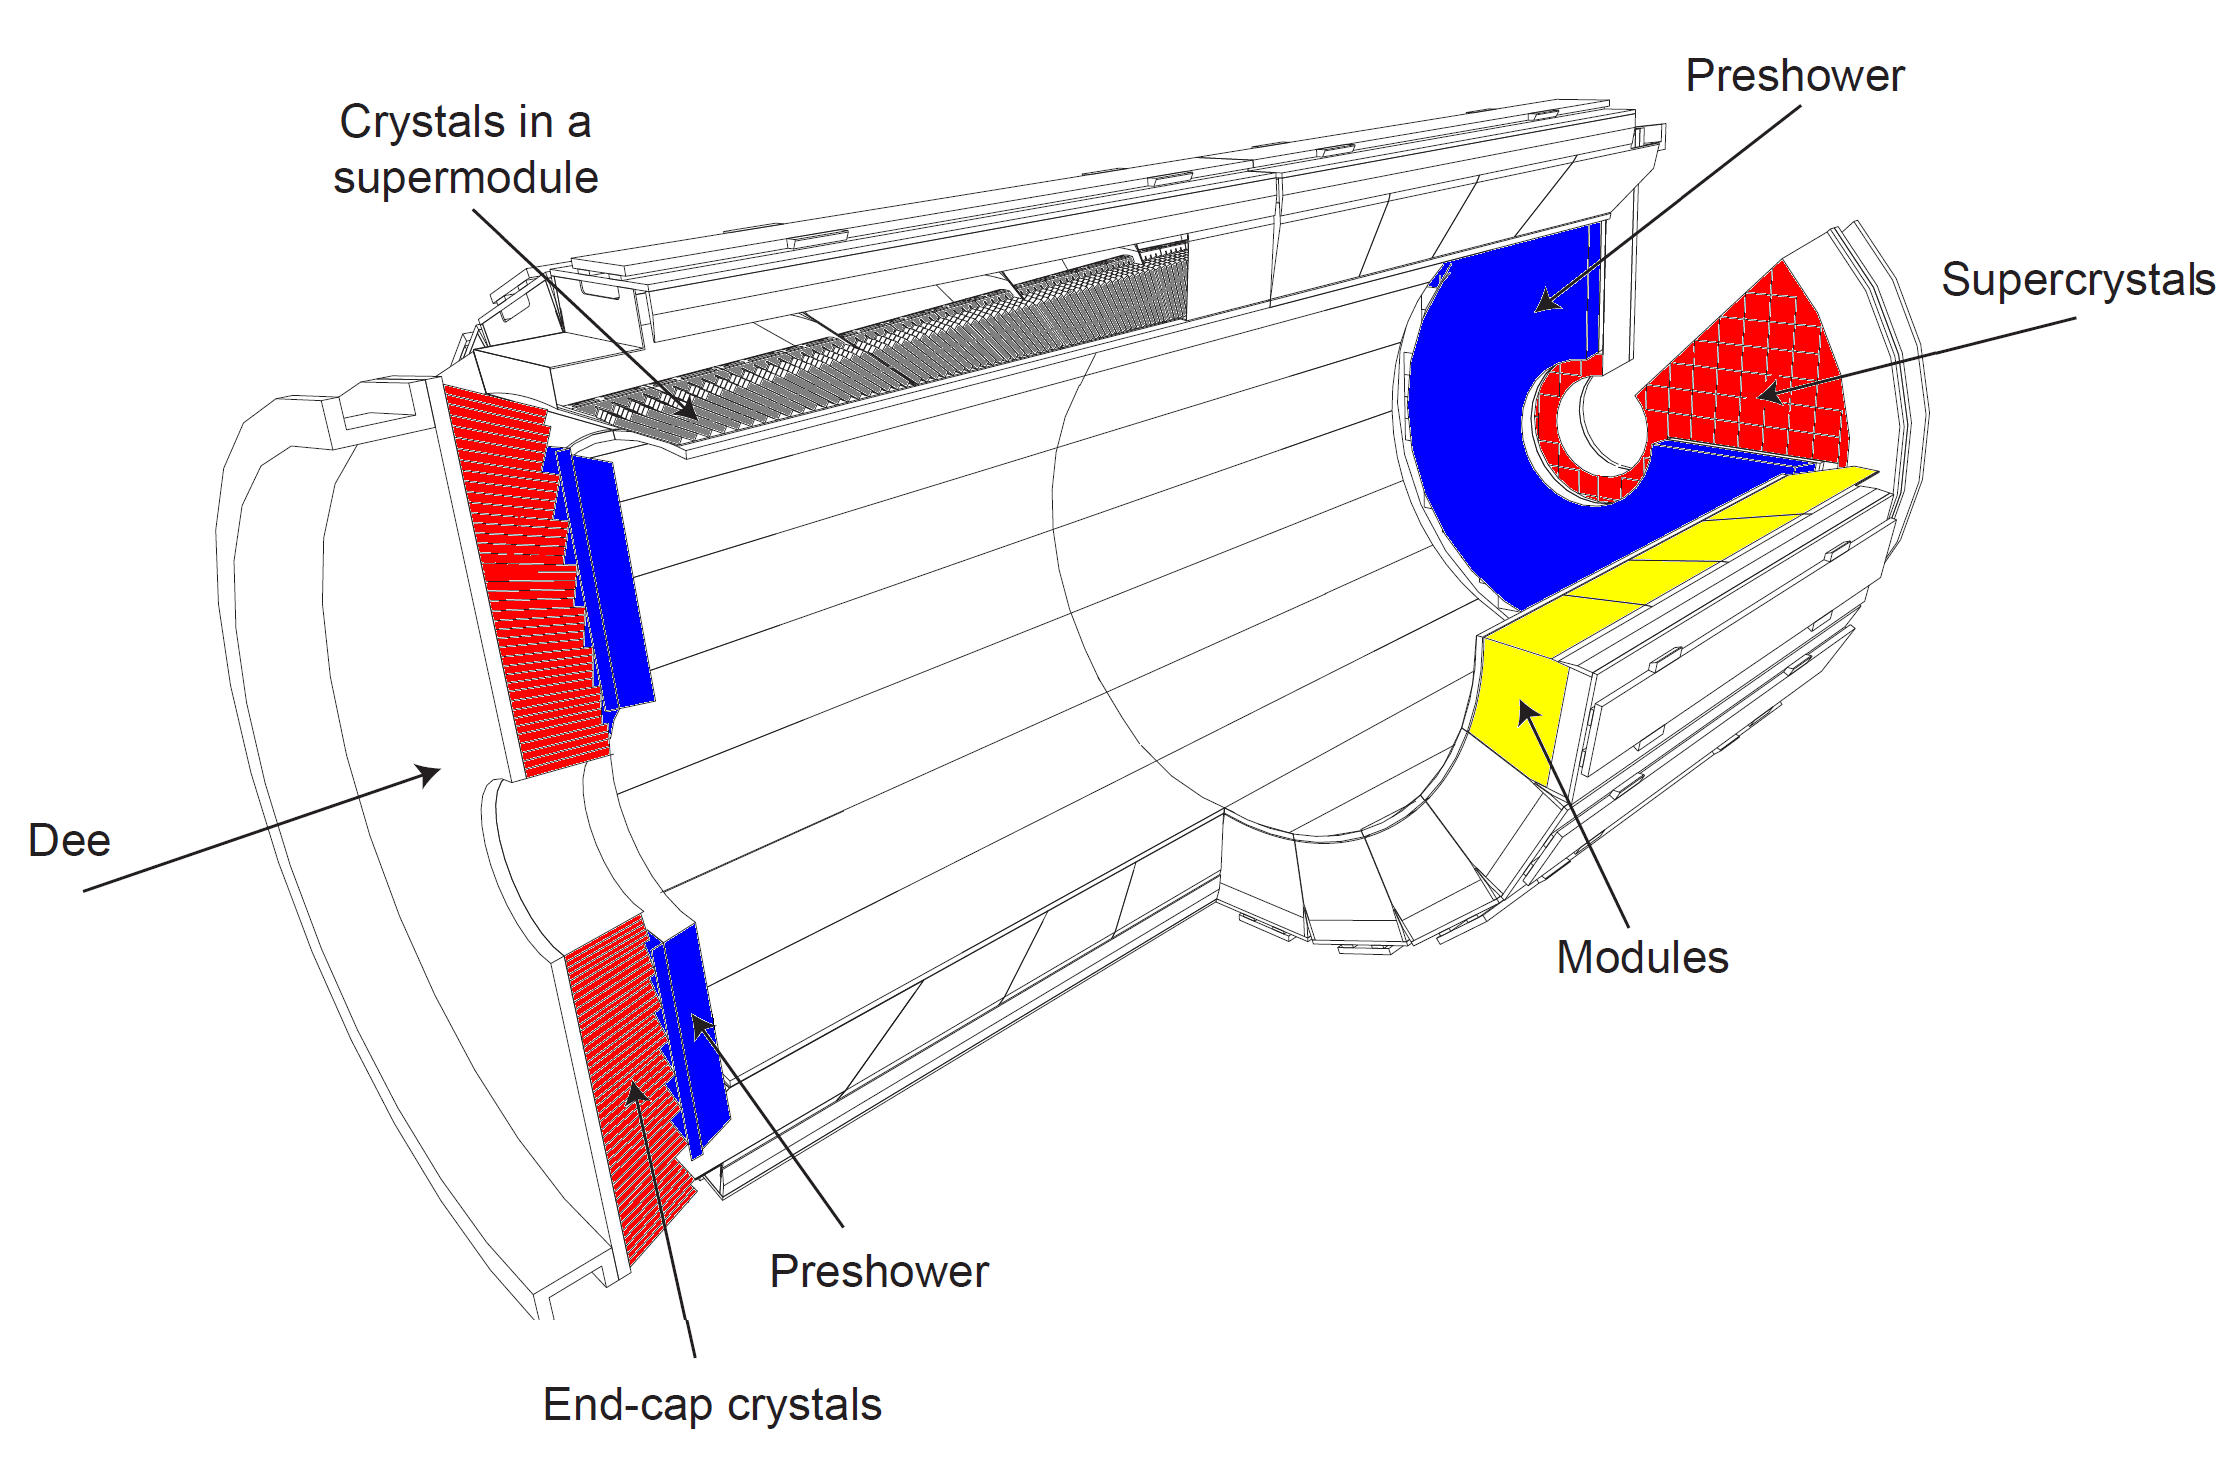
\includegraphics[scale=0.2]{ecal}
  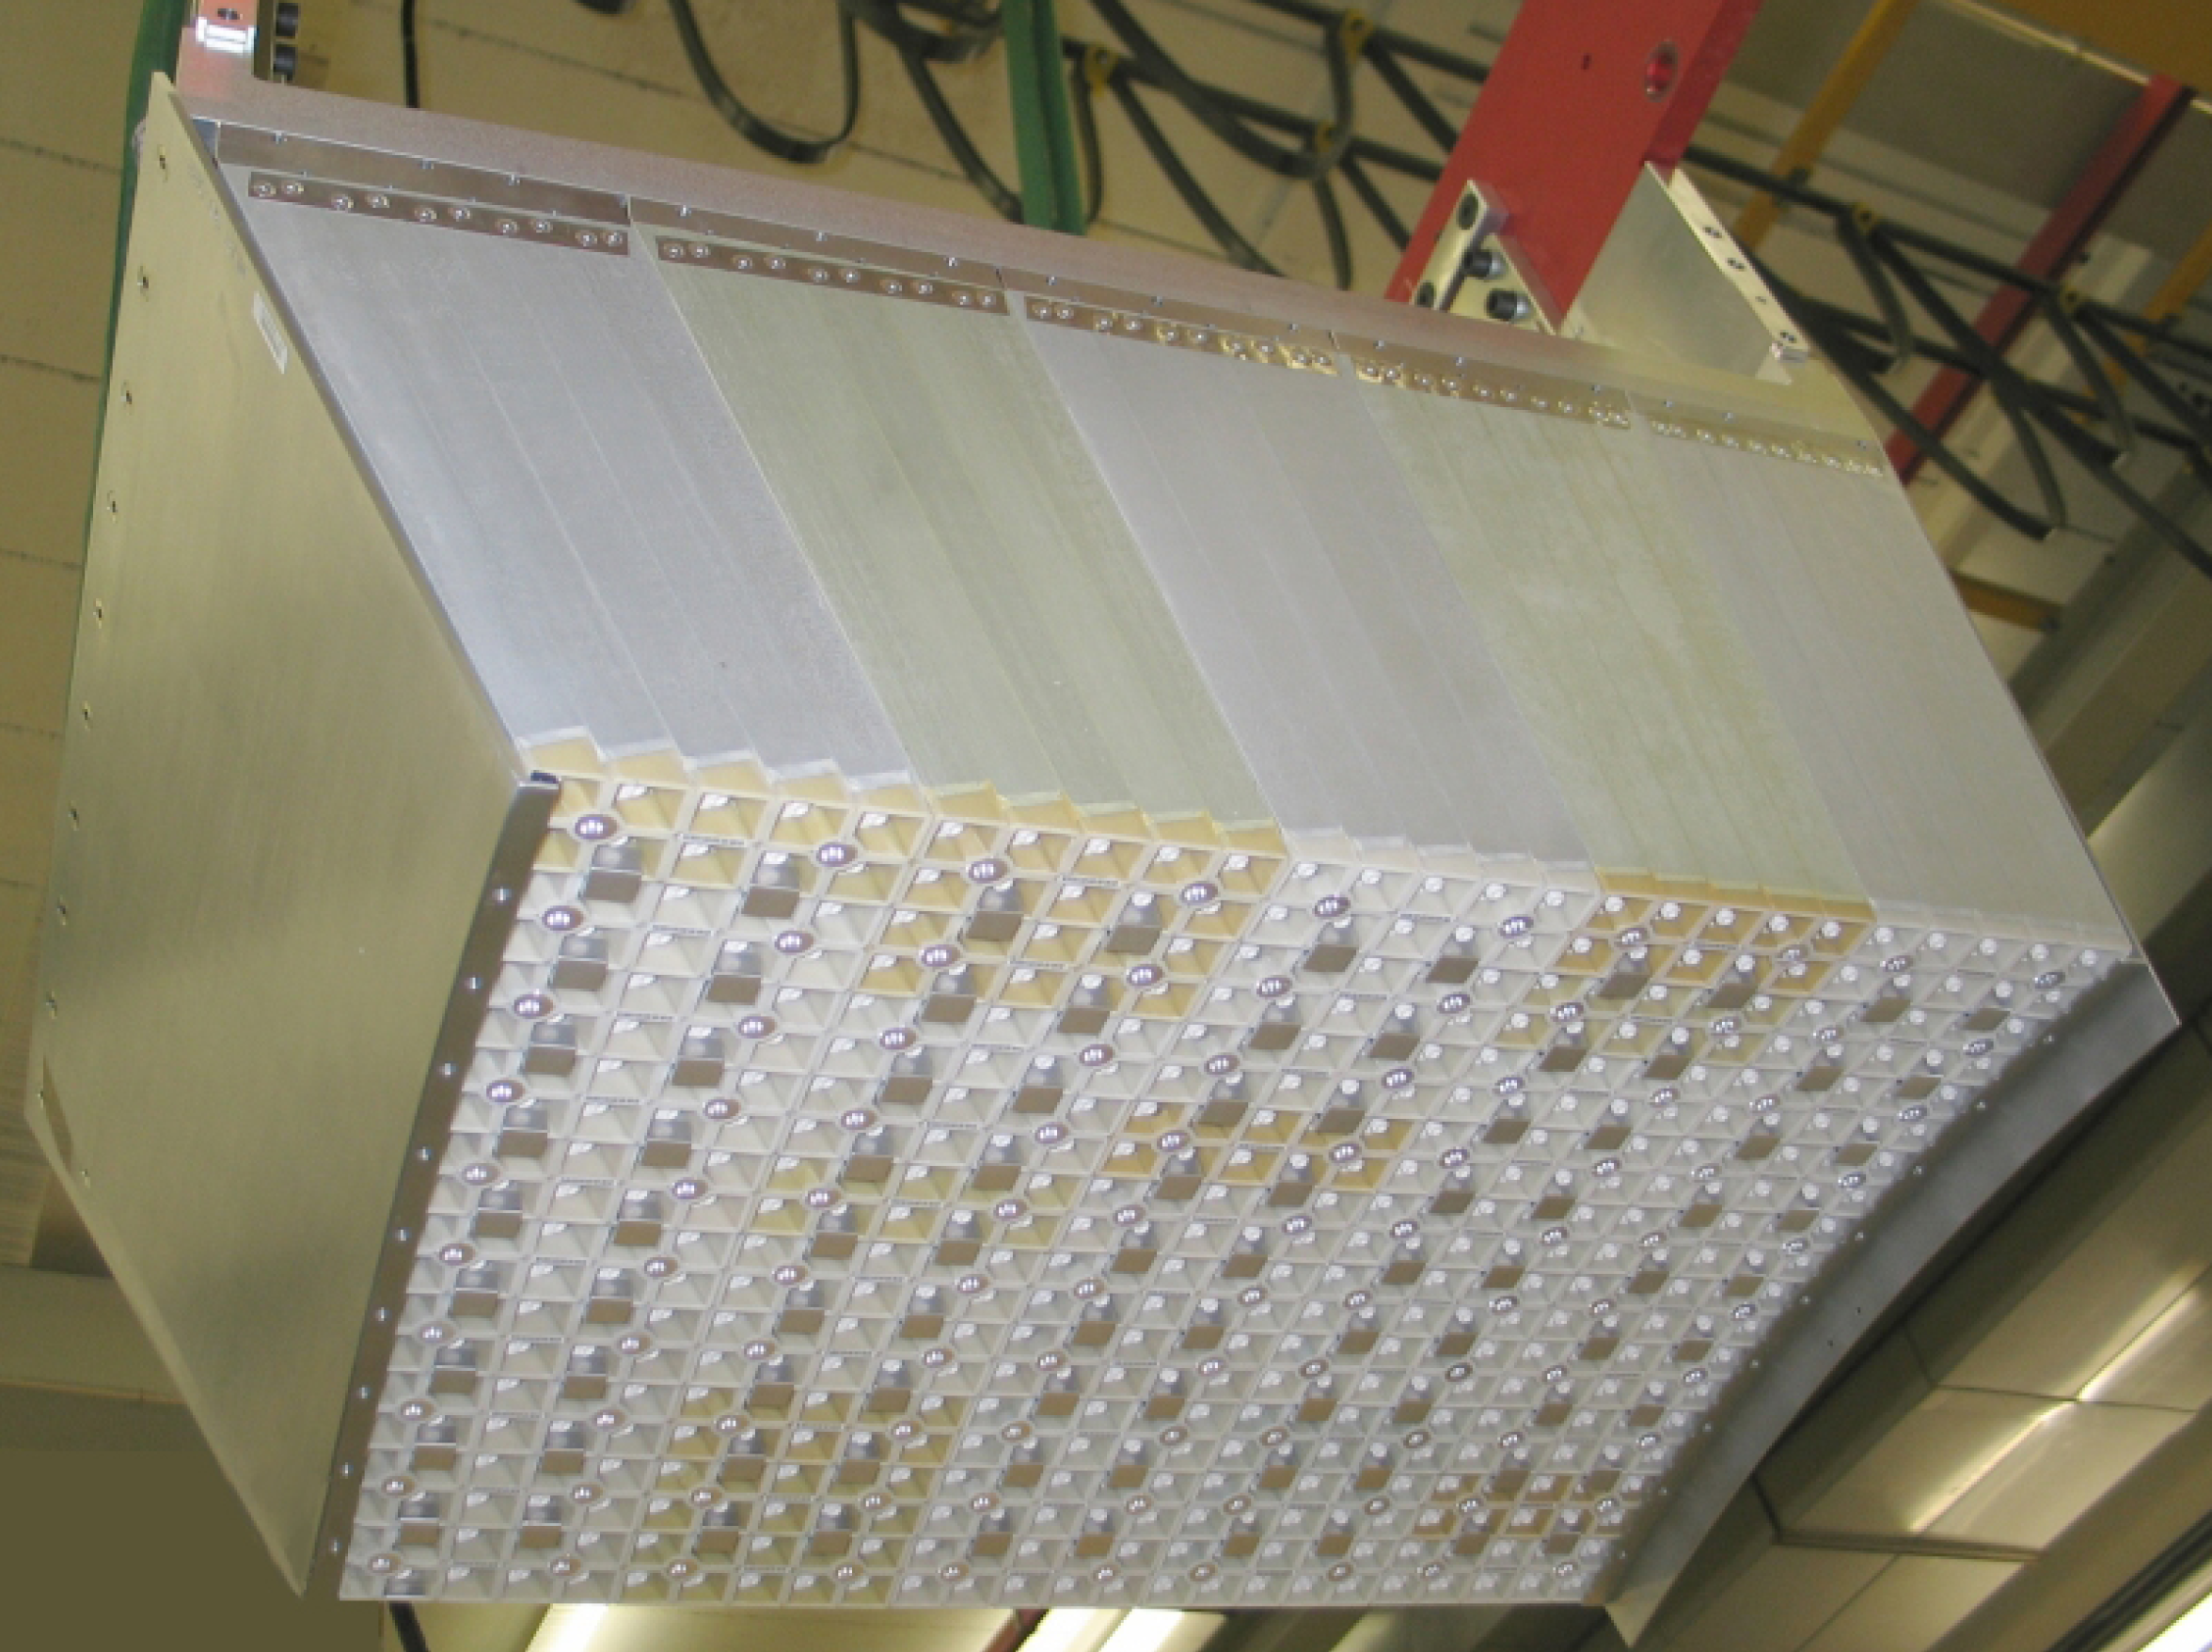
\includegraphics[width=6cm,height=4cm]{ecal_module}
  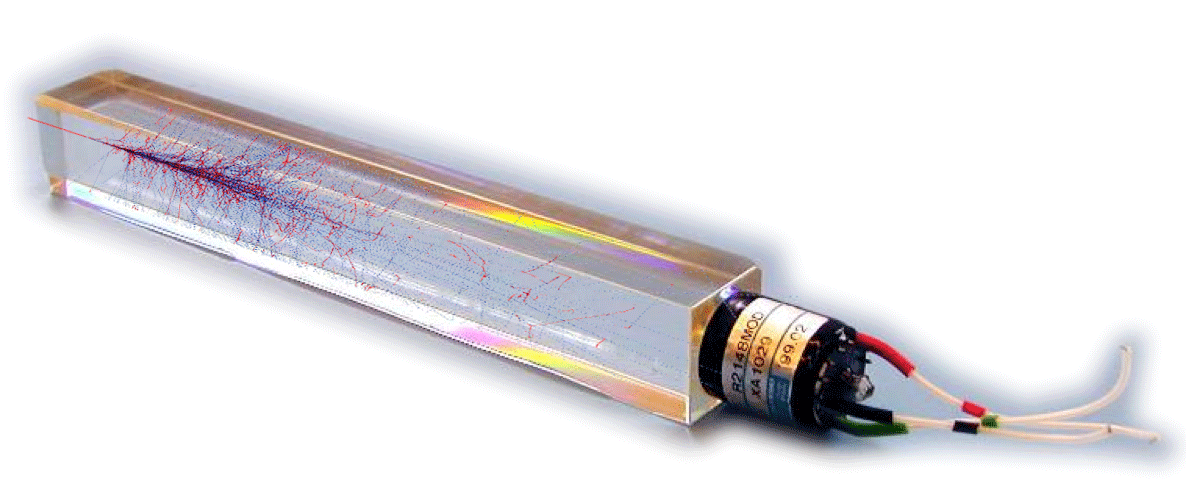
\includegraphics[width=6cm,height=4cm]{ecal_crystal} 
  \caption[CMS ECAL schematic view]{Top: CMS ECAL schematic view. Bottom: Module equipped with the crystals (left); ECAL crystal(right) with an artistic representation of an electromagnetic shower\cite{cms}.}
  \label{fig:ecal}
\end{figure}

The CMS electromagnetic calorimeter (ECAL) is designed to measure the energy of electrons and photons. It is composed of 75848 lead tungstate crystals which have a short radiation length (0.89 cm) and fast response, since 80\% of the light is emitted within 25 ns; however, they are combined with Avalanche photodiodes (APDs) as photodetectors given that crystals themselves have a low light yield (30$\gamma$/MeV). A schematic view of the ECAL is shown in Figure \ref{fig:ecal}.

Energy is measured when electrons and photons are absorbed by the crystals which generates an electromagnetic \ti{shower}, as seen in bottom right picture of the Figure \ref{fig:ecal}; the shower is seen as a \textit{cluster} of energy which depending on the amount of energy deposited can involve several crystals. The ECAL barrel (EB) covers the region $|\eta|$ < 1.479, using crystals of depth of 23 cm and  $2.2\times 2.2$ cm$^2$ transverse section; the ECAL endcap (EE) covers the region 1.479 < $|\eta|$ < 3.0 using crystals of depth 22 cm and transverse section of $2.86\times2.86$ cm$^2$; the photodetectors used are vacuum phototriodes (VPTs). Each EE is divided in two structures called \ti{Dees}.

The preshower detector (ES) is installed in front of the EE and covers the region $1.653 < |\eta| < 2.6$. The ES provides a precise measurement of the position of electromagnetic showers, which allows to distinguish electrons and photon signals from $\pi^0$ decay signals. The ES is composed of a layer of lead radiators followed by a layer of silicon strip sensors. The lead radiators initiate electromagnetic showers when reached by photons and electrons, then, the strip sensors measure the deposited energy and the transverse shower profiles. The full ES thickness is 20 cm.

\subsection{Hadronic calorimeter}

\begin{figure}[h!]
  \centering
  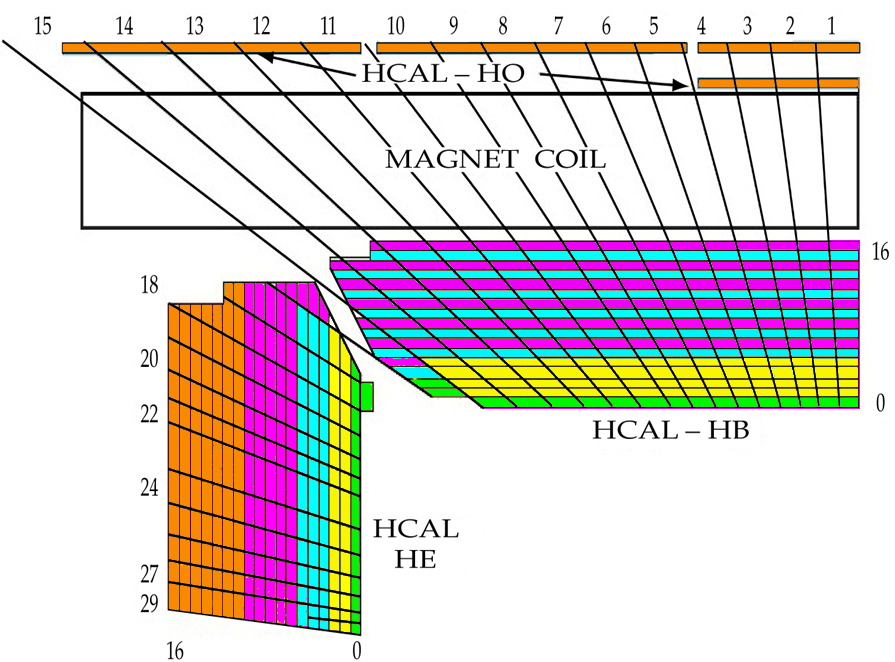
\includegraphics[scale=0.3]{hcal}\\
  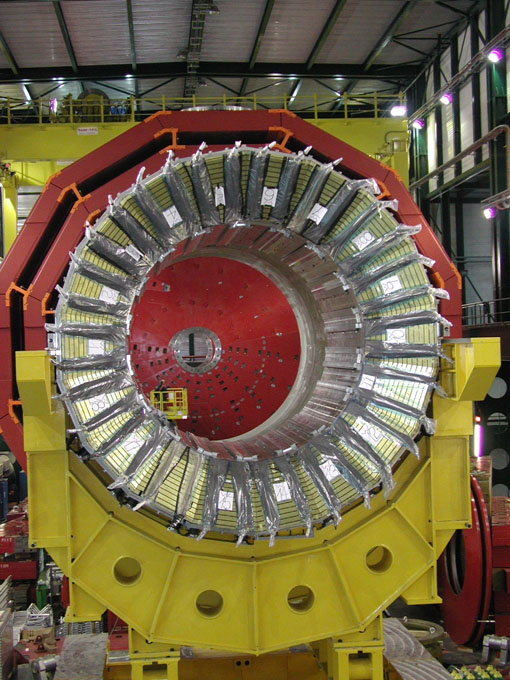
\includegraphics[width=3.5cm,height=4.5cm]{hb}
  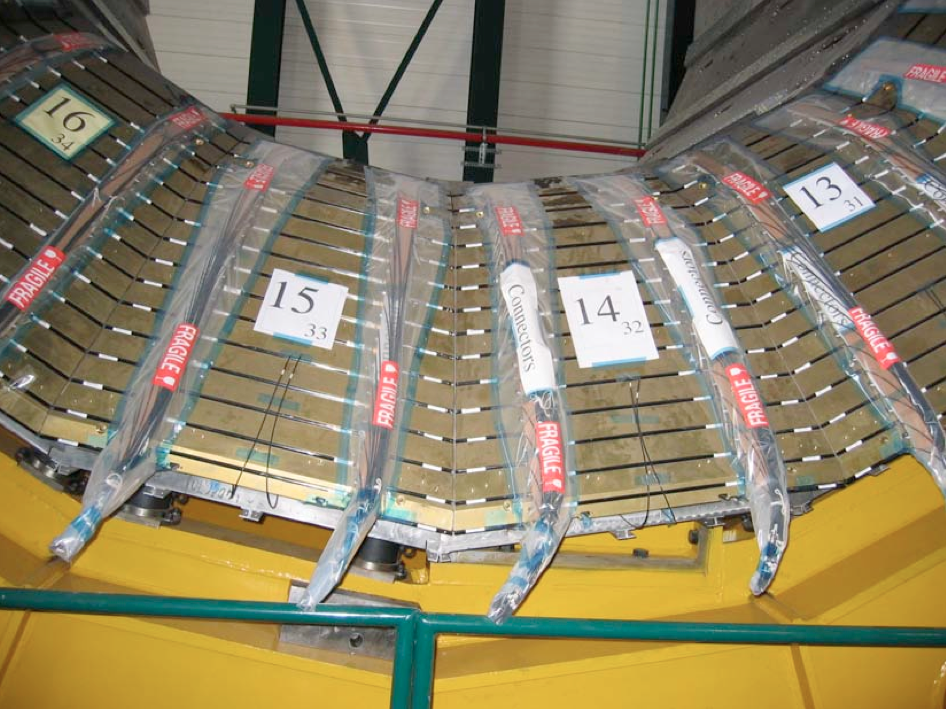
\includegraphics[width=4.5cm,height=4.5cm]{hb2}
  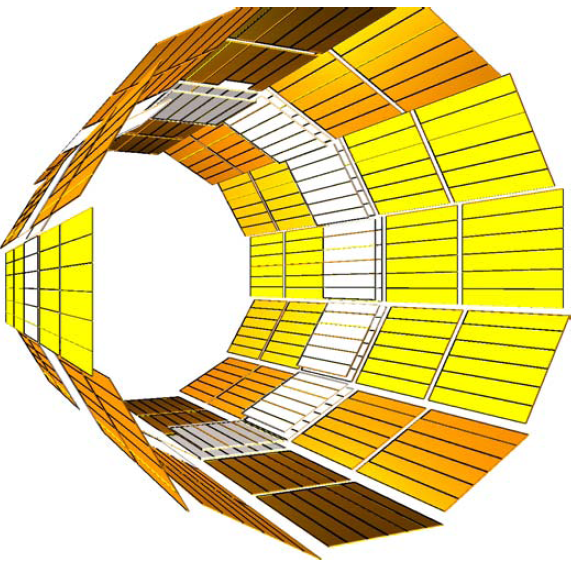
\includegraphics[width=4.5cm,height=4.5cm]{ho1} 
  \caption[CMS HCAL schematic view]{Top: CMS HCAL schematic view, the colors indicate the layers that are grouped into the same readout channels. Bottom: picture of a section of the HB; the absorber material is the golden region and scintillators are placed in between the absorber material (left and center). Schematic view of the HO (right). \cite{hcal,hb} }
  \label{fig:hcal}
\end{figure}

Hadrons are not absorbed by the ECAL\footnote{Most hadrons are not absorbed, but few low-energy ones might be.} but by the hadron calorimeter (HCAL), which is made of a combination of alternating brass absorber layers and silicon photomultiplier(SiPM) layers; therefore, particles passing through the scintillator material produce showers, as in the ECAL, as a result of the inelastic scattering of the hadrons with the detector material. Since the particles are not absorbed in the scintillator, their energy is sampled; therefore the total energy is not measured but estimated from the energy clusters, which reduces the resolution of the detector. Brass was chosen as the absorber material due to its short interaction length ($\lambda_I=16.42$ cm) and its non-magnetivity. Figure \ref{fig:hcal} shows a schematic view of the CMS HCAL.

The HCAL is divided into four sections; the Hadron Barrel (HB), the Hadron Outer (HO), the Hadron Endcap (HE) and the Hadron Forward (HF) sections. The HB covers the region $0<|\eta|<1.4$, while the HE covers the region $1.3<|\eta|<3.0$. The HF, made of quartz fiber scintillator and steel as absorption material, covers the forward region $3.0<|\eta|<5.2$. Both the HB and HF are located inside the solenoid. The HO is placed outside the magnet as an additional layer of scintillators with the purpose of measure the energy tails of particles passing through the HB and the magnet (see Figure \ref{fig:hcal} top and bottom right).% The upgrades made to the HCAL during the technical stop 2016-2017 consisted in the replacement of the photo transducer, in order to improve the efficiency.

\subsection{Superconducting solenoid magnet}

\begin{figure}[h!]
  \centering
  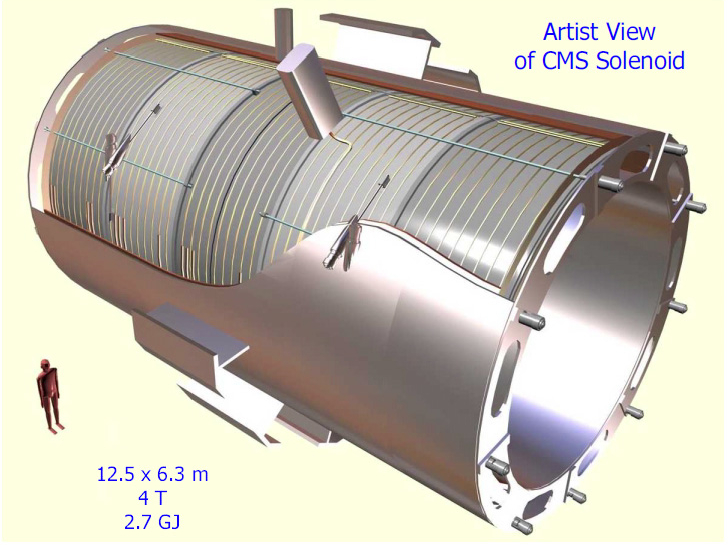
\includegraphics[scale=0.38]{magnet}
  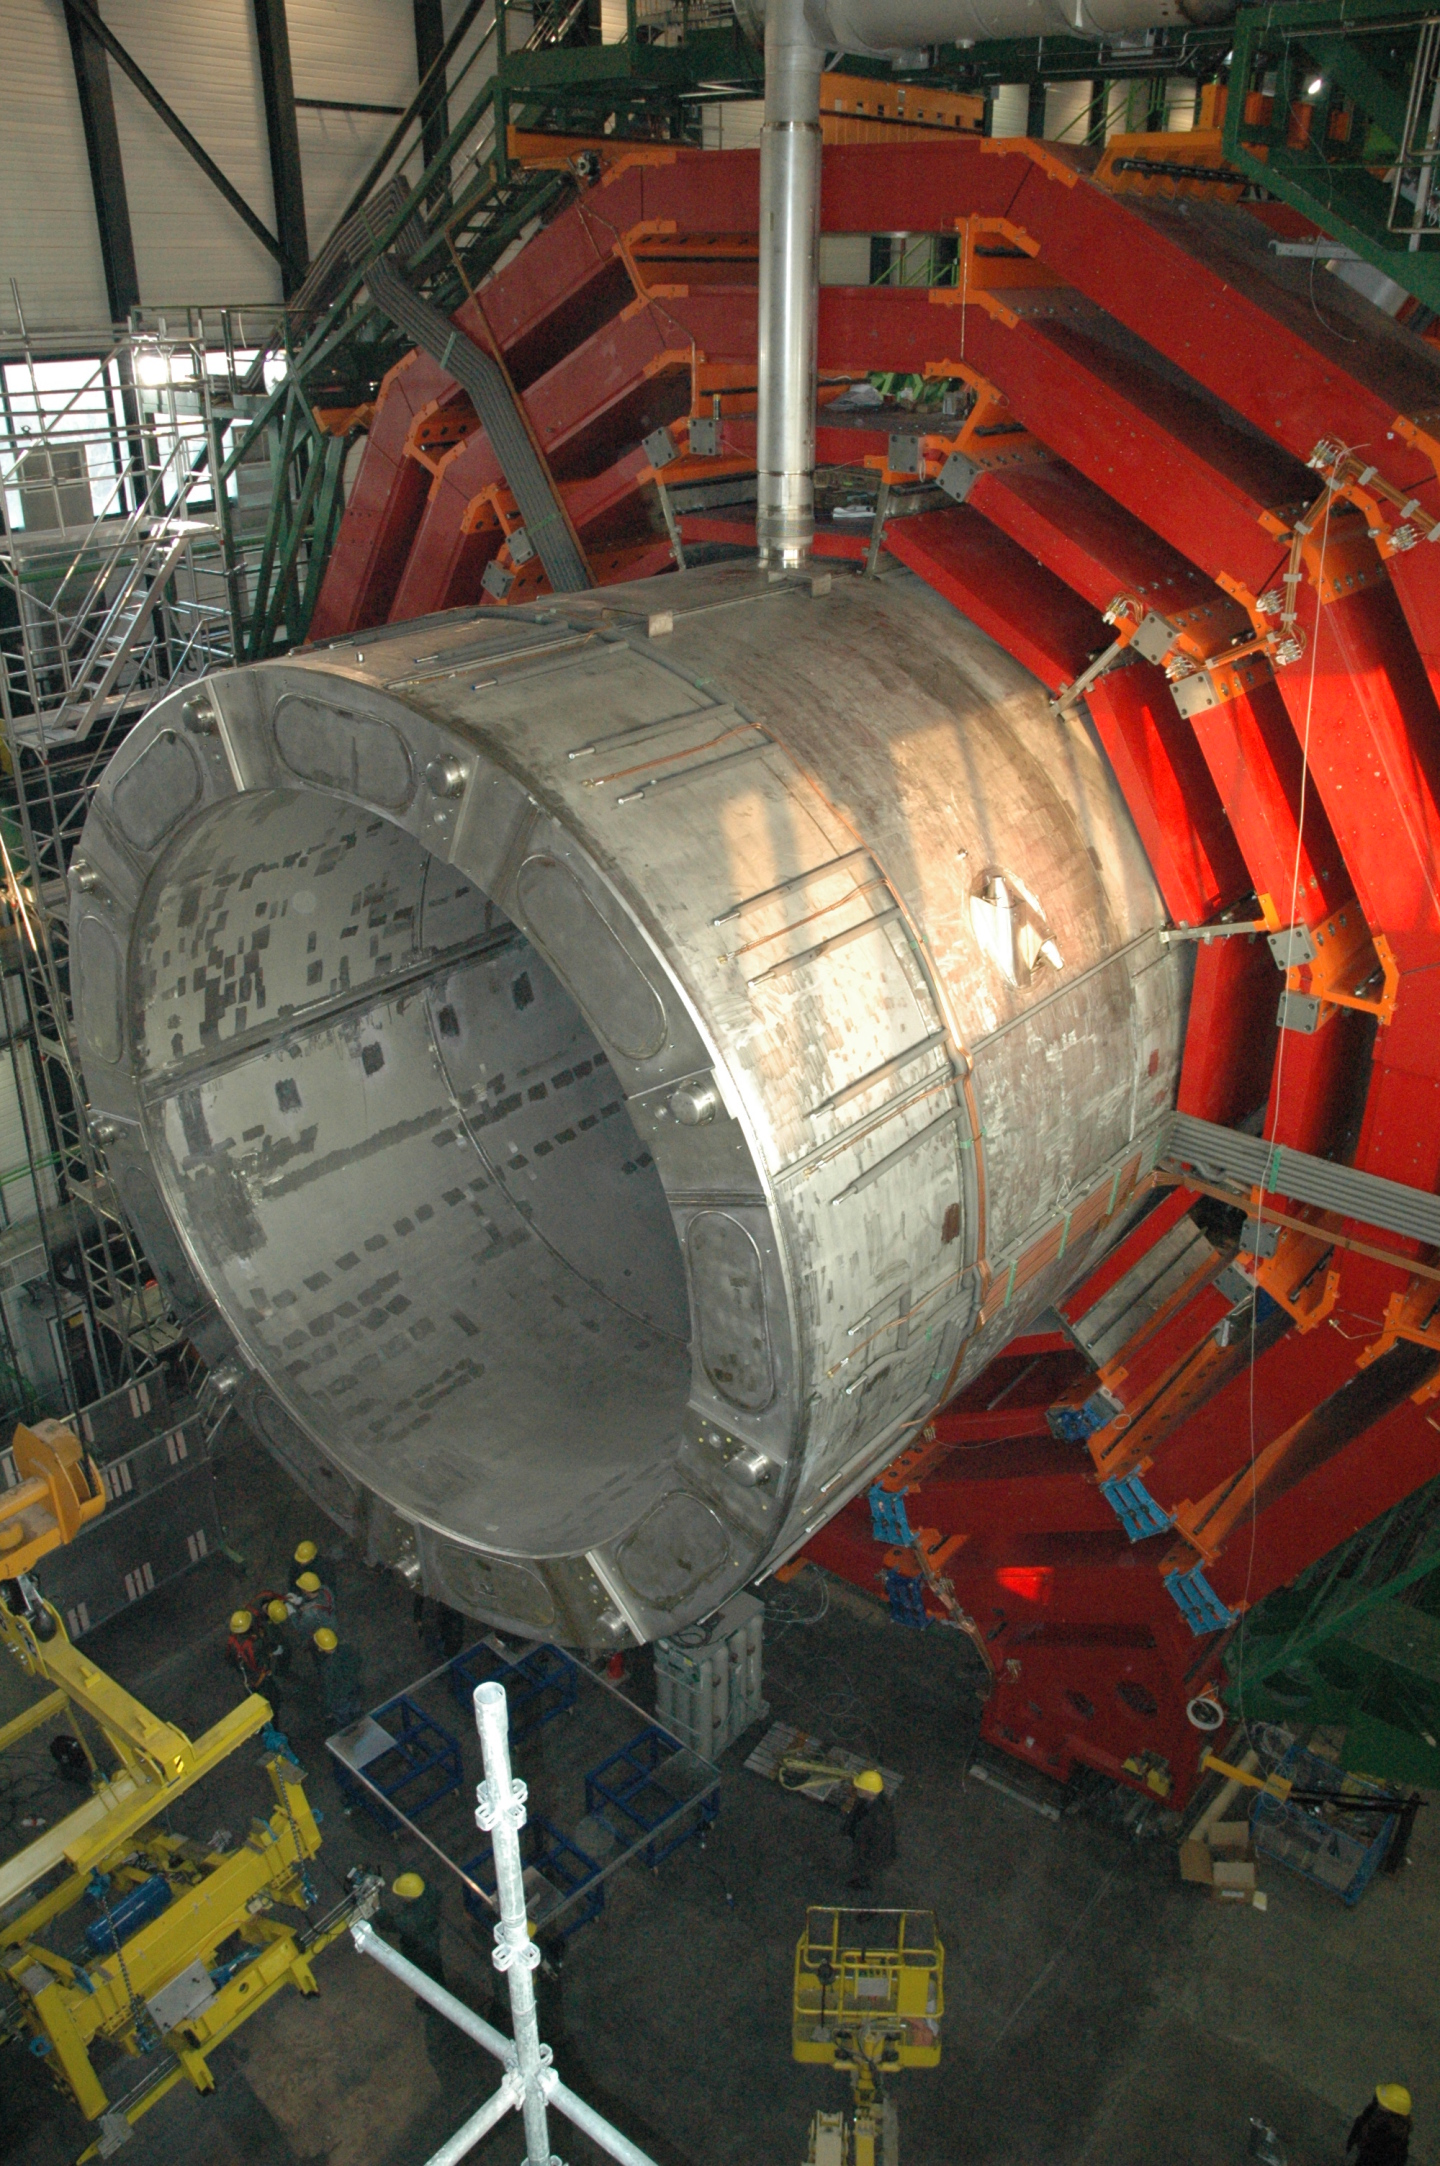
\includegraphics[scale=0.4]{yoke2}
  %\includegraphics[scale=0.4]{yoke1} 
  \caption[CMS solenoid magnet]{Artistic representation of the CMS solenoid magnet(left). The magnet is supported on an iron yoke (right) which also serves as the house of the muon detector and as mechanical support for the whole CMS detector \cite{yoke2}.}
  \label{fig:yoke}
\end{figure}

The superconducting magnet installed in the CMS detector is designed to provide an intense and highly uniform magnetic field in the central part of the detector. In fact, the tracking system takes advantage of the bending power of the magnetic field to measure with precision the momentum of the particles that traverse it; the unambiguous determination of the sign for high momentum muons was a driving principle during the design of the magnet. The magnet has a diameter of 6.3 m, a length of 12.5 m and a cold mass of 220 ton; the generated magnetic field reaches a strength of 3.8T. Since it is made of Ni-Tb superconducting cable it has to operate at a temperature of 4.7 K by using a helium cryogenic system; the current circulating in the cables reaches 18800 A under normal running conditions. The left side of Figure \ref{fig:yoke} shows an artistic view of the CMS magnet, while the right side shows a transverse view of the cold mass where the winding structure is visible.

The yoke (see Figure \ref{fig:yoke}), composed of 5 barrel wheels and 6 endcap disks made of iron, serves not only as the media for magnetic flux return but also provides housing for the muon detector system and structural stability to the full detector.     

\subsection{Muon system }

\begin{figure}[h!]
  \centering
  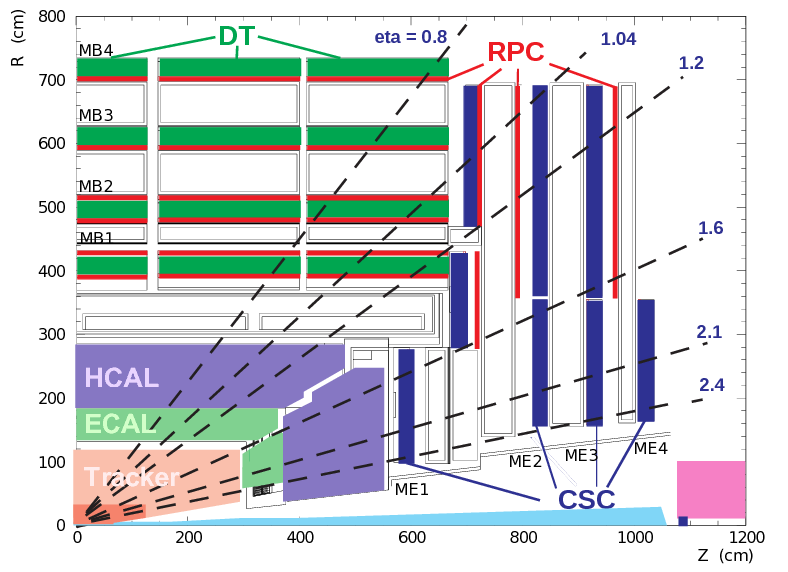
\includegraphics[width=10cm,height=6cm]{muon}
  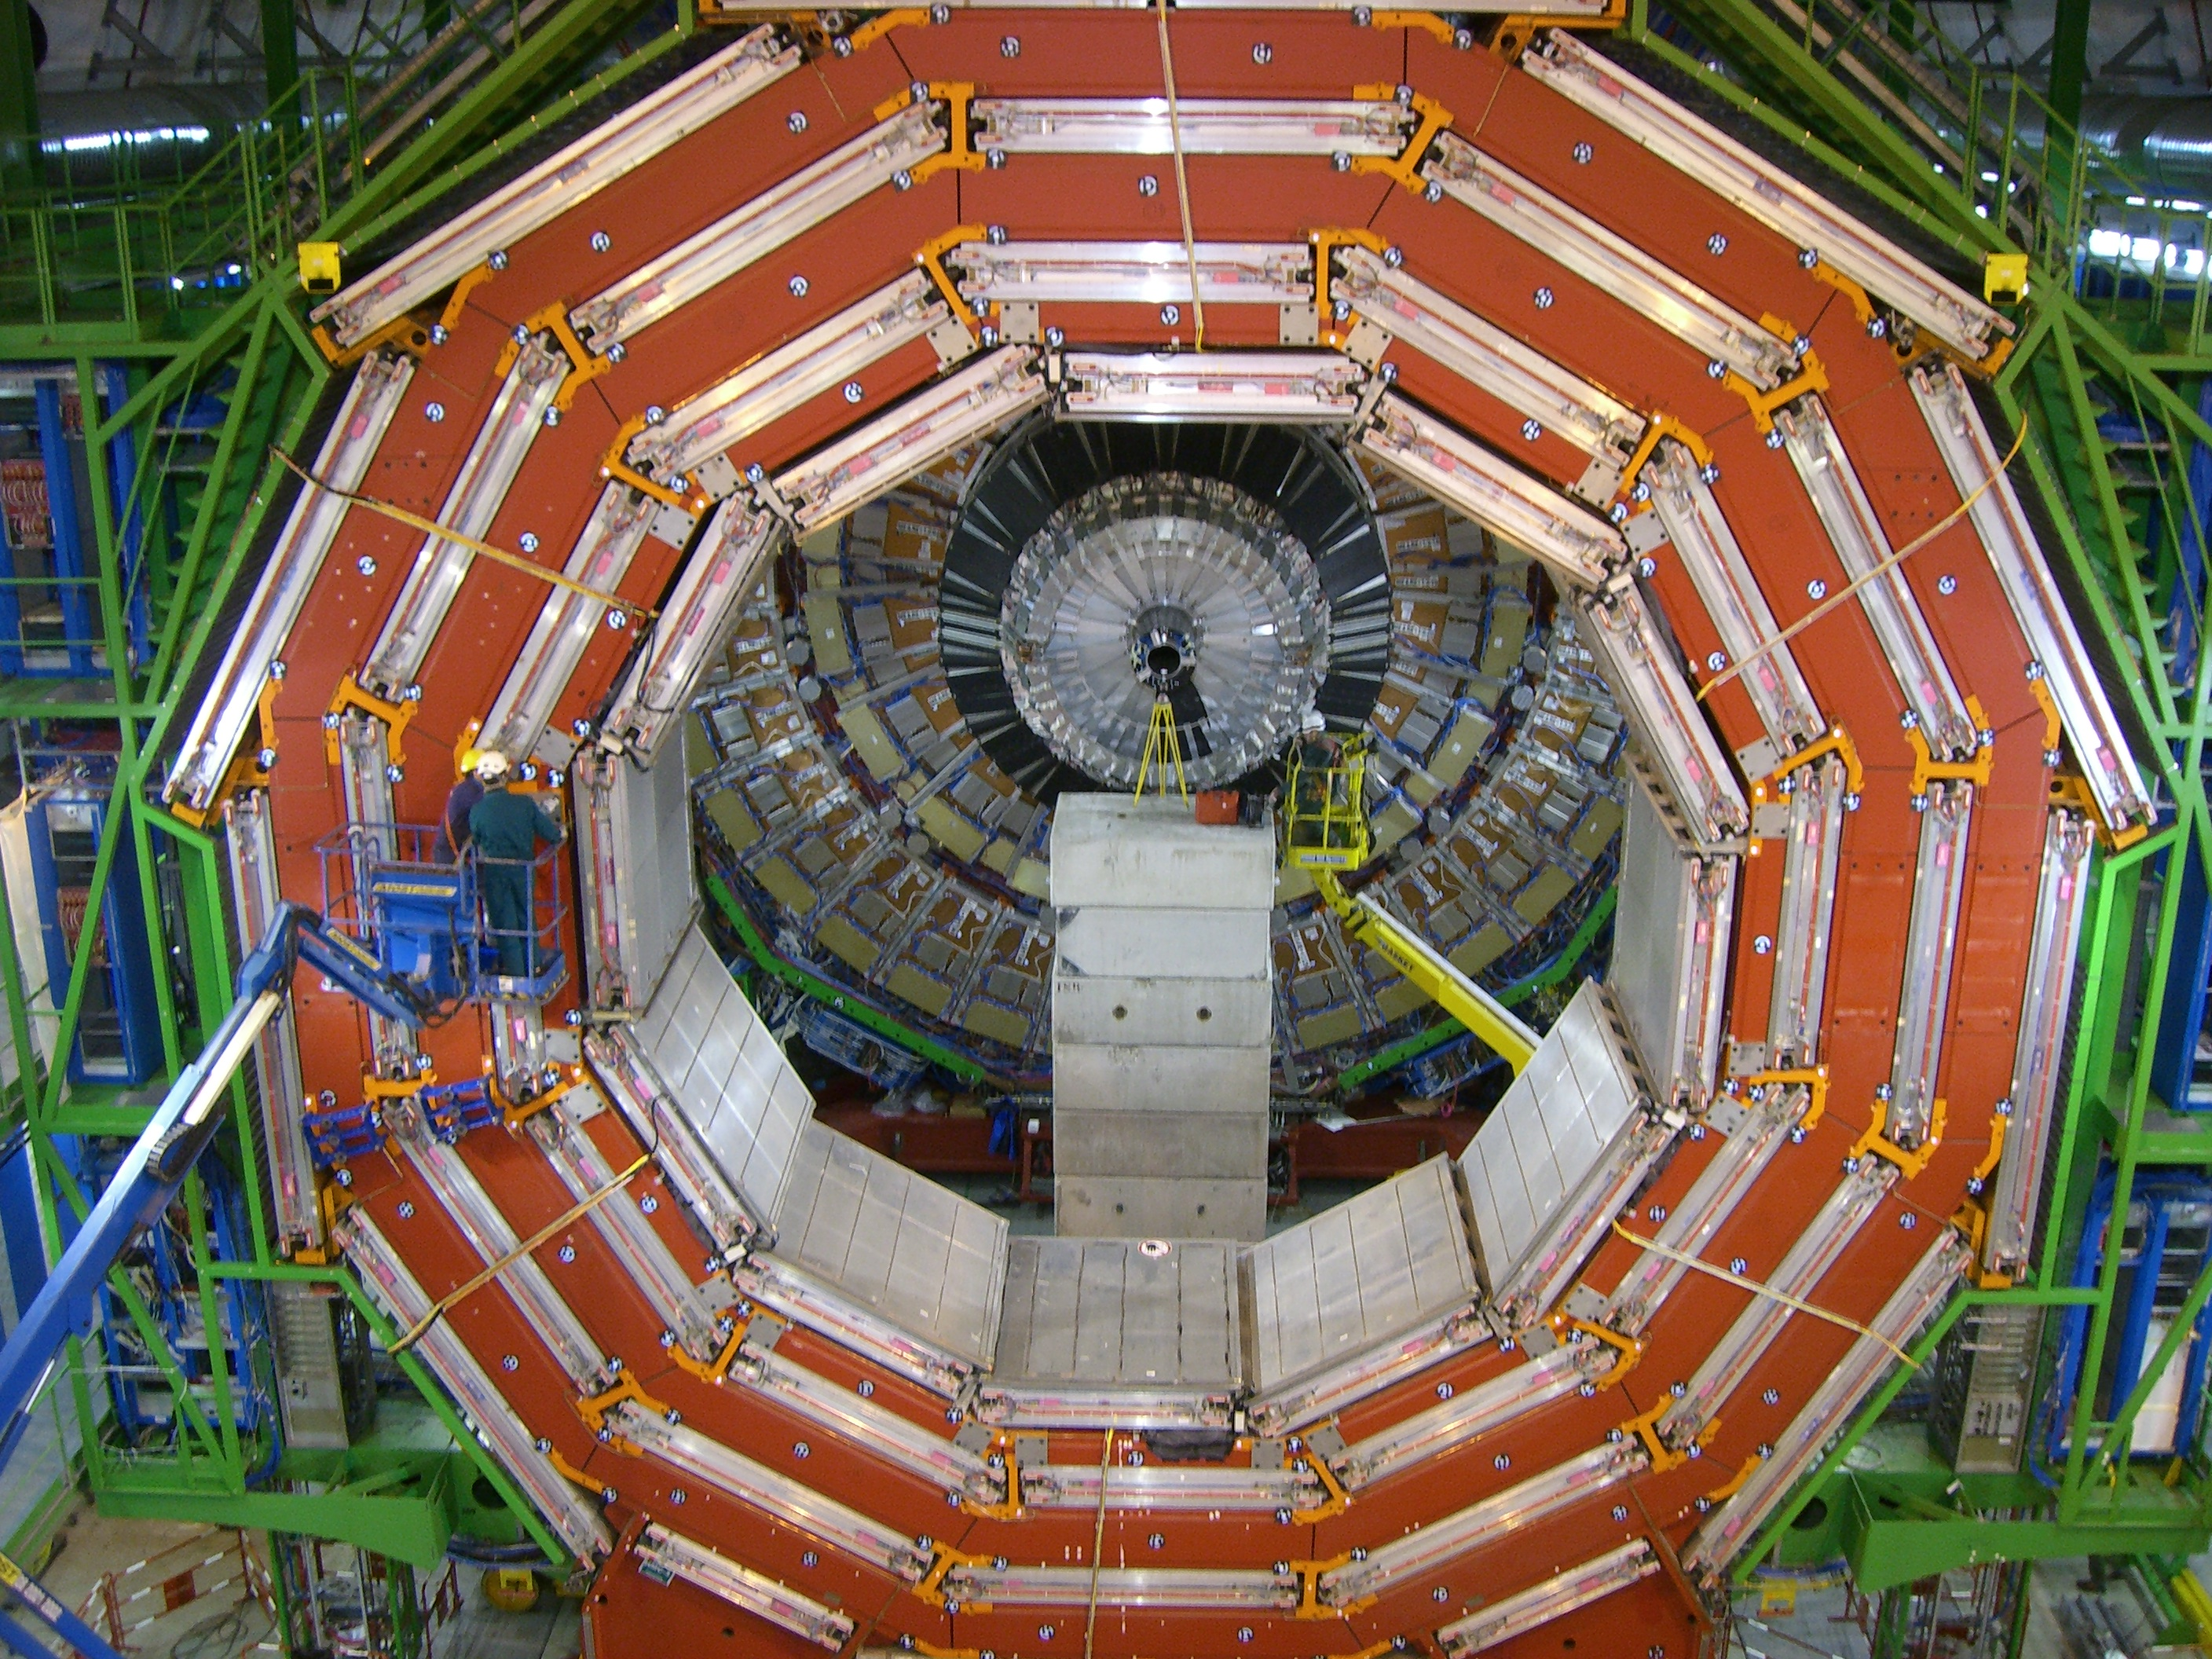
\includegraphics[width=5cm,height=4.55cm]{muon2}
  \caption[CMS Muon system schematic view]{Left: CMS muon system schematic view; Right: one of the yoke rings with the muon DTs and RPCs installed; in the back it is possible to see the muon endcap \cite{muon}. }
  \label{fig:muon_chambers}
\end{figure}

Muons are the only charged particles able to pass through all the CMS detector due to their low ionization energy loss; thus, muons can be separated easily from the high amount of particles produced in a \pp collision. Also, muons are expected to be produced in the decay of several new particles; therefore, good detection of muons was one of the leading principles when designing the CMS detector.

The CMS muon detection system (muon spectrometer) is embedded in the return yoke as seen in Figure \ref{fig:muon_chambers}. It is composed of three different detector types, the drift tube chambers (DT), cathode strip chambers (CSC), and resistive plate chambers (RPC); DT are located in the central region $\eta< 1.2$ arranged in four layers of drift chambers filled with an Ar/CO$_2$ gas mixture.

The muon endcaps are made of CSCs covering the region $\eta< 2.4$ and filled with a mixture of Ar/CO$_2$/CF$_4$. The reason behind using a different detector type lies on the different conditions in the forward region like the higher muon rate and higher residual magnetic field compared to the central region.

The third type of detector used in the muon system is a set of four disks of RPCs working in avalanche mode. The RPCs provide good spatial and time resolutions. The track of high-$p_T$ muon candidates is built combining information from the tracking system and the signal from up to six RPCs and four DT chambers.

The muon tracks are reconstructed from the hits in the several layers of the muon system. 

\subsection{CMS trigger system}

CMS expects \pp collisions every 25 ns, \ie, an interaction rate of 40 MHz for which it is not possible to store the recorded data in full. In order to handle this high event rate data, an online event selection, known as triggering, is performed; triggering reduces the event rate to 100 Hz for storage and further offline analysis.        

The trigger system starts with a reduction of the event rate to 100 kHz in the so-called \ti{ the level 1 trigger} (L1). L1 is based on dedicated programmable hardware like Field Programmable Gate Arrays (FPGAs) and Application Specific Integrated Circuits (ASICs), partly located in the detector itself; another portion is located in the CMS underground cavern. Hit pattern information from the muon chambers and the energy deposits in the calorimeter are used to decide if an event is accepted or rejected, according to selection requirements previously defined, which reflect the interesting physics processes. Figure \ref{fig:l1} shows the L1 trigger architecture.

\begin{figure}[h!]
  \centering
  \includegraphics[width=10cm,height=6cm]{l1}
  \caption[CMS Level-1 trigger architecture]{CMS Level-1 trigger architecture \cite{l1}. }
  \label{fig:l1}
\end{figure}

The second stage in the trigger system is called \ti{the high-level trigger} (HLT); events accepted by L1 are passed to HLT in order to make an initial reconstruction of them. HLT is software based and runs on a dedicated server farm, using selection algorithms and high-level object definitions; the event rate at HLT is reduced to 100 Hz. The first HLT stage takes information from the muon detectors and the calorimeters to make the initial object reconstruction; in the next HLT stage, information from the pixel and strip detectors is used to do first fast tracking and then full tracking online. This initial object reconstruction is used in further steps of the trigger system.

Events and preliminary reconstructed physics objects from HLT are sent to be fully reconstructed at the CERN computing center know also as Tier-0 facility. Again, the pixel detector information provides high-quality seeds for the track reconstruction algorithm offline, primary vertex reconstruction, electron and photon identification, muon reconstruction, $\tau$ identification, and b-tagging. After full reconstruction, data sets are made available for offline analyses.

Sometimes, a trigger \ti{prescale} is introduced in order to reduce even further the event rate; thus, for a prescaling of ten only one of each ten events passing the trigger requirements is saved.    
%During the 2016-2017 technical stop, the L1 system was updated in order to improve the physics object identification by improving the algorithms and accounting for the increasing pile-up scenario.  

\subsection{CMS computing}

Data coming from the experiment have to be stored and made available for further analysis; in order to cope with all the tasks implied in the offline data processing, like transfer, simulation, reconstruction and reprocessing, among others, a large computing power is required. The CMS computing system is based on the distributed architecture concept, where users of the system and physical computer centers are distributed worldwide and interconnected by high-speed networks.

\begin{figure}[h!]
  \centering
  \includegraphics[scale=0.4]{WLCG}
  \caption[WLCG structure]{WLCG structure. The primary computer centers (Tier-0) are located at CERN (data center) and at the Wigner datacenter in Budapest. Tier-1 is composed of 13 centers and Tier-2 is composed of about 160 centers. \cite{wlcg}. }
  \label{fig:wlcg}
\end{figure}

The worldwide LHC computing grid (WLCG) is the mechanism used to provide that distributed environment. WLCG is a tiered structure connecting computing centers around the world, which provides the necessary storage and computing facilities. The primary computing centers of the WLCG are located at the CERN and the Wigner datacenter in Budapest and are known as Tier-0 as shown in Figure \ref{fig:wlcg}. The main responsibilities for each tier level are \cite{wlcg}

\begin{itemize}
\item \textbf{Tier-0}: initial reconstruction of recorded events and storage of the resulting datasets, the distribution of raw data to the Tier-1 centers.
\item \textbf{Tier-1}: provide storage capacity, support for the Grid, safe-keeping of a proportional share of raw and reconstructed data, large-scale reprocessing and safe-keeping of corresponding output, generation of simulated events, distribution of data to Tier 2s, safe-keeping of a share of simulated data produced at these Tier 2s.
\item \textbf{Tier-2}: store sufficient data and provide adequate computing power for specific analysis tasks and proportional share of simulated event production and reconstruction.
\end{itemize}

Aside from the general computing strategy to manage the huge amount of data produced by experiments, CMS uses a software framework to perform a variety of processing, selection and analysis tasks. The central concept of the CMS data model referred to as \ti{event data model} (EDM) is the \ti{Event}; therefore, an event is the unit that contains the information from a single bunch crossing, any data derived from that information like the reconstructed objects, and the details of the derivaction.

Events are passed as the input to the \ti{physics modules} that obtain information from them and create new information; for instance, \ti{event data producers} add new data into the events, \ti{analyzers} produce an information summary from an event set, \ti{filters} perform selection and triggering.

CMS uses several event formats with different levels of detail and precision

\begin{itemize}
\item \textbf{Raw format}: events in this format contain the full recorded information from the detector as well as trigger decision and other metadata. An extended version of raw data is used to store information from the CMS Monte Carlo simulation tools (see Chapter \ref{ch:gensimreco}). Raw data are stored permanently, occupying about 2MB/event   
\item \textbf{RECO format}: events in this format correspond to raw data that have been submitted to reconstruction algorithms like primary and secondary vertex reconstruction, particle ID, and track finding. RECO events contain physics objects and all the information used to reconstruct them; average size is about 0.5 MB/event.     
\item \textbf{AOD format}: Analysis Object Data (AOD) is the data format used in the physics analyses given that it contains the parameters describing the high-level physics objects in addition to enough information to allow a kinematic refitting if needed. AOD events are filtered versions of the RECO events to which skimming or other filtering have been applied, hence AOD events are subsets of RECO events. Requires about 100 kB/event.
\item \textbf{Non-event data} are data needed to interpret and reconstruct events. Some of the non-event data used by CMS contains information about the detector contraction and condition data like calibrations, alignment, and detector status.  
\end{itemize}

\noindent Figure \ref{fig:dataflow} shows the data flow scheme between CMS detector and tiers.

\begin{figure}[h!]
  \centering
  \includegraphics[scale=0.4]{dataflow}
  %\includegraphics[scale=0.15]{dataflow2}
  \caption[Data flow from CMS detector through hardware Tiers]{Data flow from CMS detector through tiers.}
  \label{fig:dataflow}
\end{figure}


\noindent  The whole collection of software built as a framework is referred to as \ti{CMSSW}. This framework provides the services needed by the simulation, calibration and alignment, and reconstruction modules that process event data, so that physicists can perform analysis. The CMSSW event processing model is composed of one executable, called cmsRun, and several plug-in modules which contains all the tools  (calibration, reconstruction algorithms) needed to process an event. The same executable is used for both detector data and Monte Carlo simulations \cite{cmssw}.
